\chapter{\label{chapter:6_Results}Results}

In this chapter, we will present the results of our experimental evaluation of our cases of study presented in Chapters~\ref{chapter:4_work-stealing} and~\ref{chapter:5_modular-basket-queues}. We will provide an in-depth analysis of the data we collected. We have gained valuable insights into our research topic through rigorous testing and analysis. We believe that the results presented in this chapter will contribute to a better understanding of the subject matter and will pave the way for future research in this field. So, let us dive in and explore the outcomes of our study in detail.

\section{Work-Stealing with Multiplicity}

First, we present a summary of the experimental evaluation results from the Case of Study presented in Chapter~\ref{chapter:4_work-stealing}:

\begin{itemize}
\item Zero cost experiments. In both experiments, \Puts{}-\Takes{} and \Puts-\Steals{}, overall, the algorithm with the best performance was \NCWSM, followed by \NCWSM Lists and then idempotent FIFO, regardless of the initial array size. This result is expected because \NCWSM does not use either costly primitives or memory fences. It was also observed that idempotent FIFO performed better than \NCWSM Lists when no resizing was needed. \BNCWSM and \BNCWSM Lists performed worst among all algorithms. However, this did not preclude them from exhibiting a competitive performance in the second and third benchmarks.

\item Parallel spanning tree. In virtually all experiments, \NCWSM performed best among all tested algorithms. It outperformed Cilk THE and Chase-Lev, performing better than \NCWSM Lists and idempotent FIFO by small margins. Idempotent FIFO performed best among the idempotent algorithms.  \BNCWSM exhibited a competitive performance. Work-stealing algorithms with FIFO policy generally showed low amounts of repeated work. In contrast, algorithms with LIFO of dequeue policies exhibited higher amounts, and, for some graphs, the difference with FIFO is remarkable.

\item Parallel SAT. In general, all work-stealing algorithms enhanced performance, and in both relaxations, repeated work was negligible, which resulted in minor performance overhead. The algorithms showed no significant statistical difference in performance for large-size assignments (i.e., fairly complex jobs associated with tasks).

\end{itemize}

The following subsections explain the results of the experiments in detail.

\subsection{Zero Cost Experiment}


The outcome of the \Puts{}-\Takes{} experiment appears in Figures~\ref{fig:putstakes:256}, \ref{fig:putstakes:1000000} and \ref{fig:putstakes:10000000}.  Overall, the absence of fences in \NCWSM derived an improvement over idempotent algorithms that range between 9\% to 65\%. Table~\ref{puts-takes-percentage} contains the percentage improvement of \NCWSM over all algorithms. In all cases, \BNCWSM and \BNCWSM Lists performed worst. This is arguably attributed to the extra array of boolean flags used for bounding multiplicity.~\footnote{Implementations where the two arrays are consolidated in a single array of objects with two entries, a task, and a flag, performed even worse. Hence, these implementations were discarded.}  It was also observed that the data structure's initial size impacts performance. When the initial size exceeds the number of operations in the experiment (Figure~\ref{fig:putstakes:10000000}), no resizes are needed, \BNCWSM's performance improved considerably. Still, it was affected by the use of two distinct arrays. The outcome of the \Puts{}-\Steal{}{} experiment is similar, and shown in Figures~\ref{fig:putssteals:256}, \ref{fig:putssteals:1000000} and \ref{fig:putssteals:10000000}, and Table~\ref{puts-steals-percentage}. %\ref{sec:results-zero-cost} contains the detailed measurements of each algorithm in each experiment.

\begin{table}[!ht]
\centering
\resizebox{\textwidth}{!}{\begin{tabular}{lrrrrrrrrr}
\toprule{} &  Chase-Lev &  Cilk THE &  Idempotent FIFO &  Idempotent LIFO &  Idempotent DEQUE &  WS WMult &  B. WS WMult &  WS WMult Lists &  B. WS WMult Lists \\
\midrule
\textbf{Intial zize 256:       } &      48.00 &     49.26 &            51.85 &            42.90 &             65.64 &      0.00 &        88.75 &           52.14 &              71.46 \\
\textbf{Initial size 1,000,000: } &      45.48 &     46.82 &            48.73 &            41.77 &             62.34 &      0.00 &        87.83 &           40.41 &              65.45 \\
\textbf{Initial size 10,000,000:} &      27.91 &     27.14 &            14.31 &            43.81 &             50.25 &      0.00 &        71.22 &           46.76 &              75.19 \\
\bottomrule
\end{tabular}}

\caption{\label{puts-takes-percentage}
Percentage improvement of $\sf \small WS\hbox{-}WMULT$ over all algorithms
in the $\Puts$-$\Takes$ experiment.}
%achieved by the best algorithm (WS WMult), compared to other algorithms in the Put-Takes experiments is shown in these values. Each row corresponds to different initial sizes.}
\end{table}


\begin{table}[!ht]
\centering
\resizebox{\textwidth}{!}{\begin{tabular}{lrrrrrrrrr}
\toprule{} &  Chase-Lev &  Cilk THE &  Idempotent FIFO &  Idempotent LIFO &  Idempotent DEQUE &  WS WMult &  B. WS WMult &  WS WMult Lists &  B. WS WMult Lists \\
\midrule
\textbf{Intial size 256:       } &      46.22 &     63.68 &            50.66 &            51.66 &             66.60 &      0.00 &        89.47 &           52.60 &              76.53 \\
\textbf{Initial size 1,000,000:} &      43.91 &     62.91 &            48.25 &            51.67 &             64.03 &      0.00 &        88.81 &           40.90 &              70.53 \\
\textbf{Initial size 10,000,000:} &      24.86 &     57.88 &             9.00 &            53.67 &             52.61 &      0.00 &        75.03 &           46.32 &              77.75 \\
\bottomrule
\end{tabular}}

\caption{\label{puts-steals-percentage}
Percentage improvement of $\sf \small WS\hbox{-}WMULT$ over all algorithms
in the $\Puts$-$\Steals$ experiment.}
%The percentage improvement achieved by the best algorithm (WS WMult), compared to other algorithms in the Puts-Steals experiments is shown in these values. Each row corresponds to different initial sizes.}
\end{table}


\begin{figure}[!ht]
  \subfloat[\label{fig:putstakes:256}Puts and Takes with an initial size 256]{
    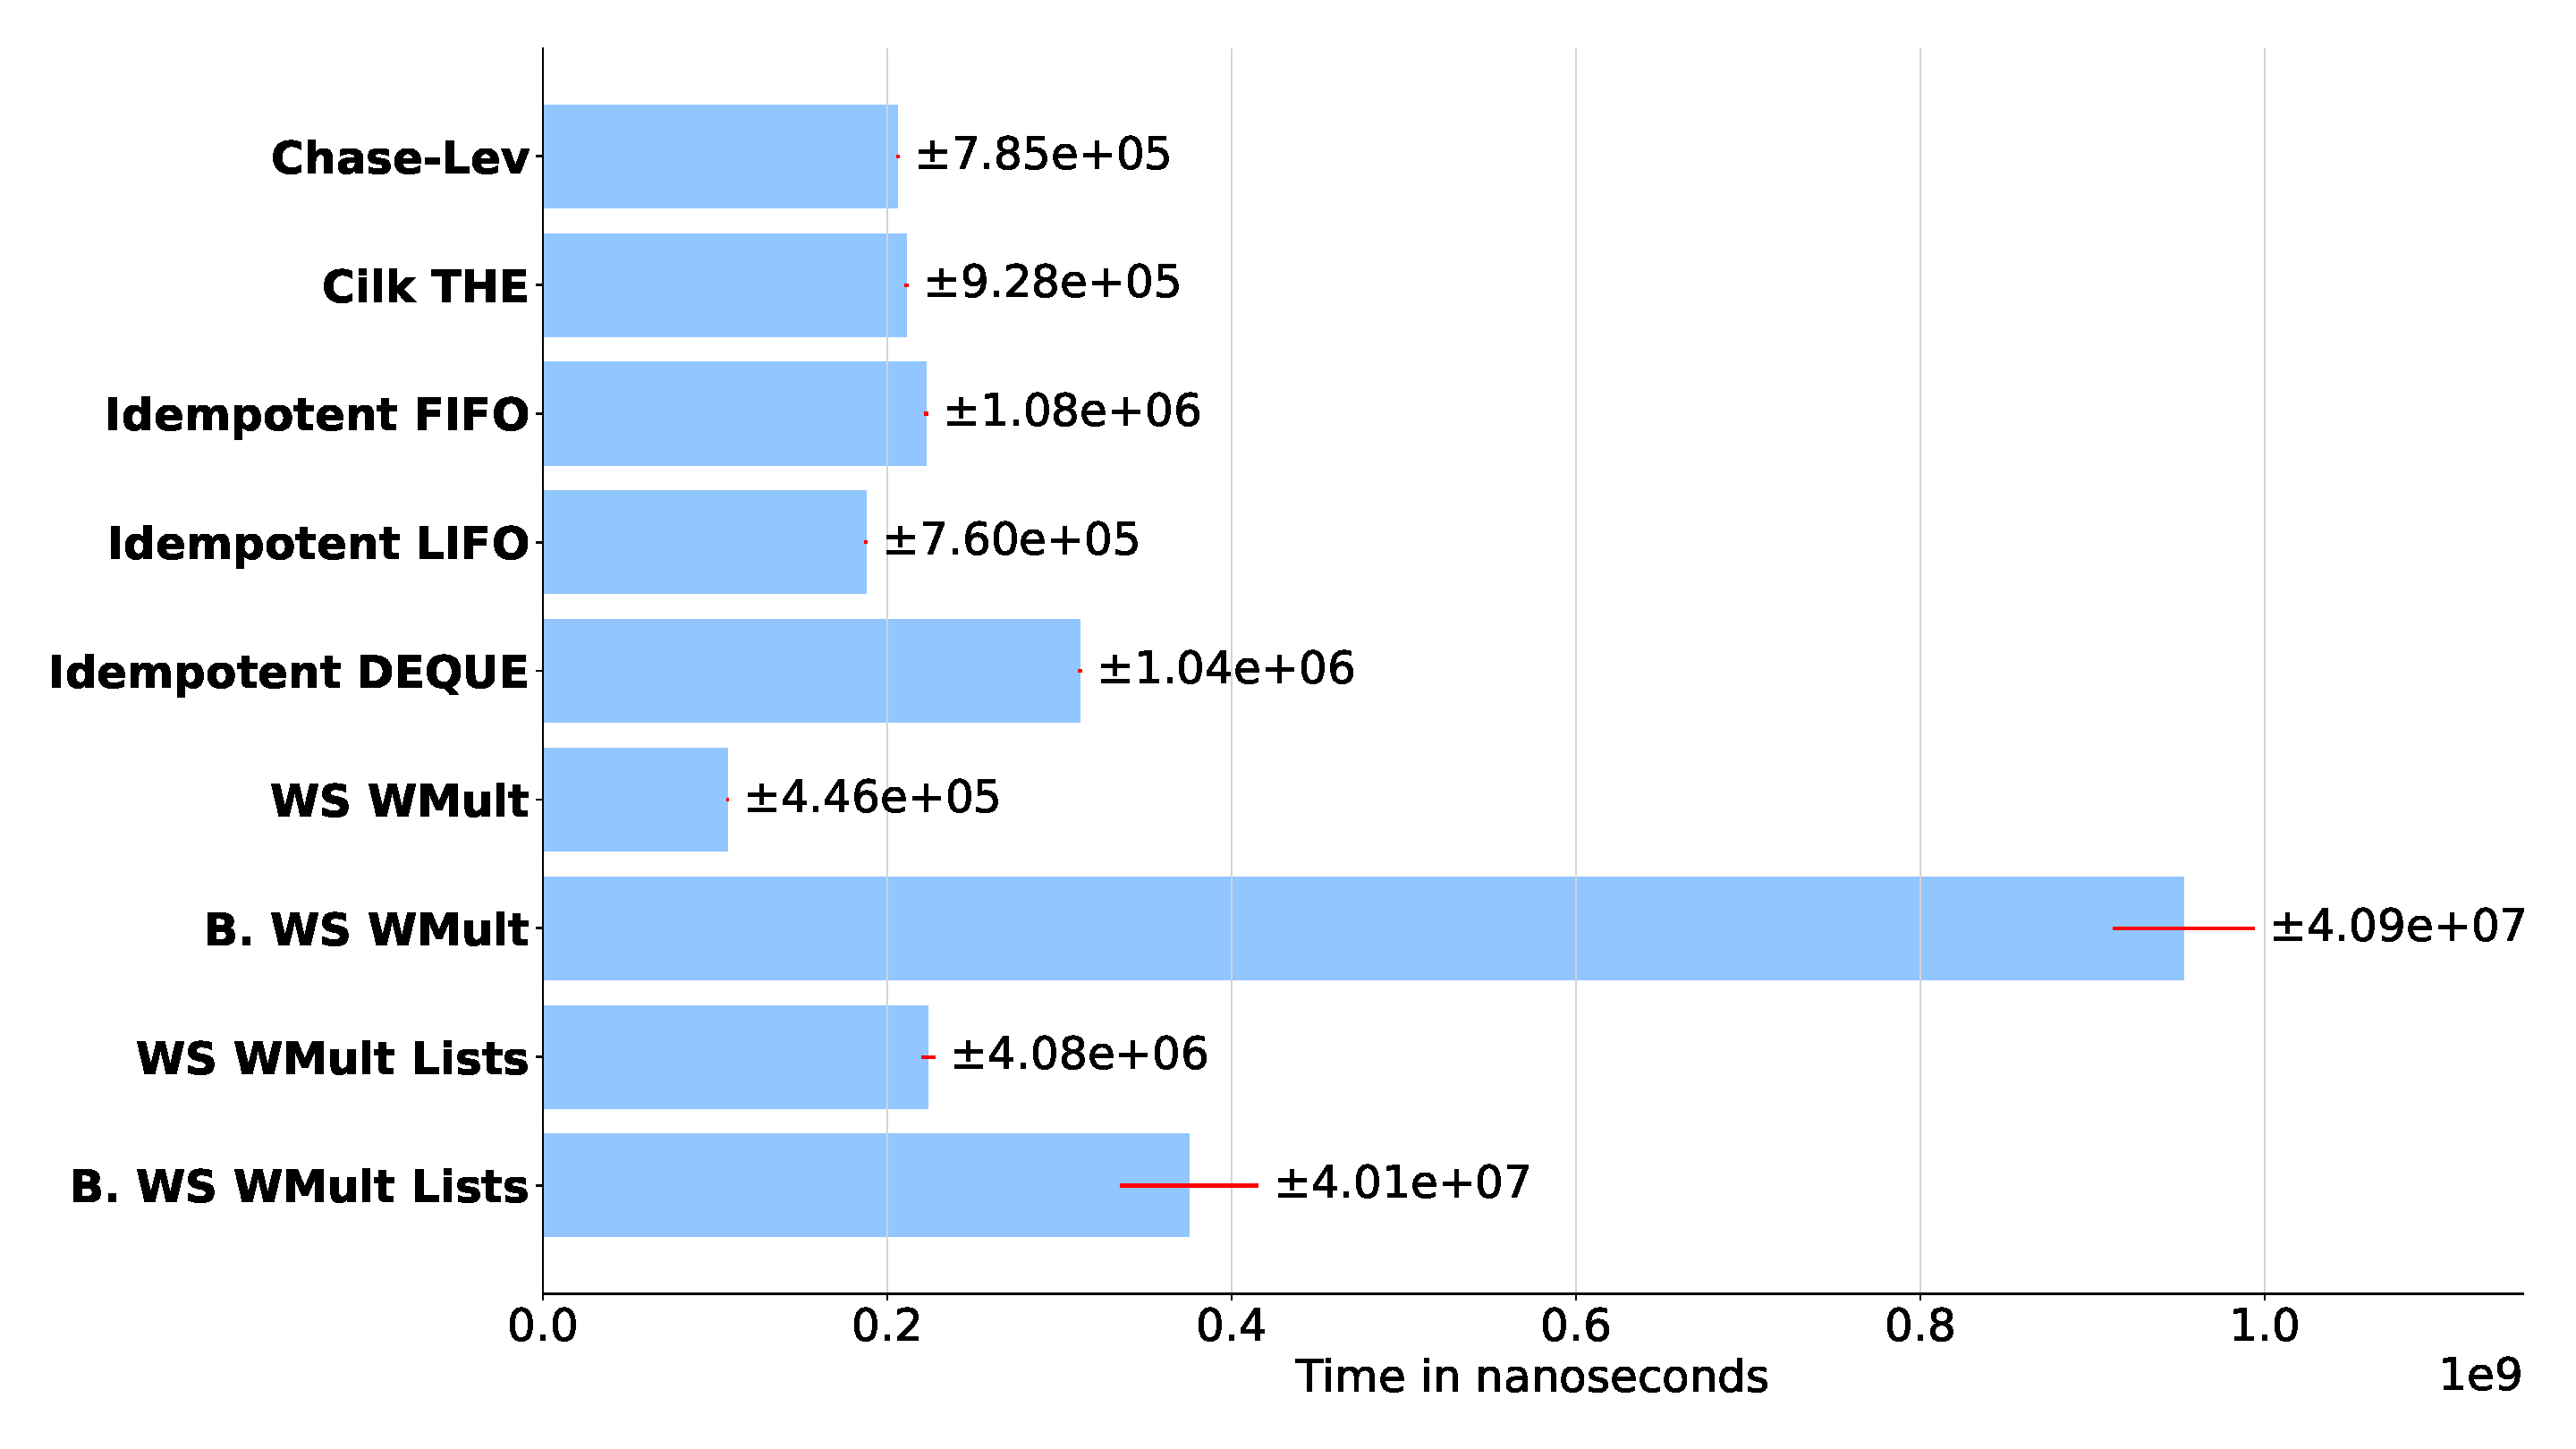
\includegraphics[width=0.47\textwidth]{contents/figures/IV_6_chart-puts-takes-256-10000000.pdf}
  }
  \subfloat[\label{fig:putstakes:1000000}Puts and Takes with an initial size 1,000,000]{
    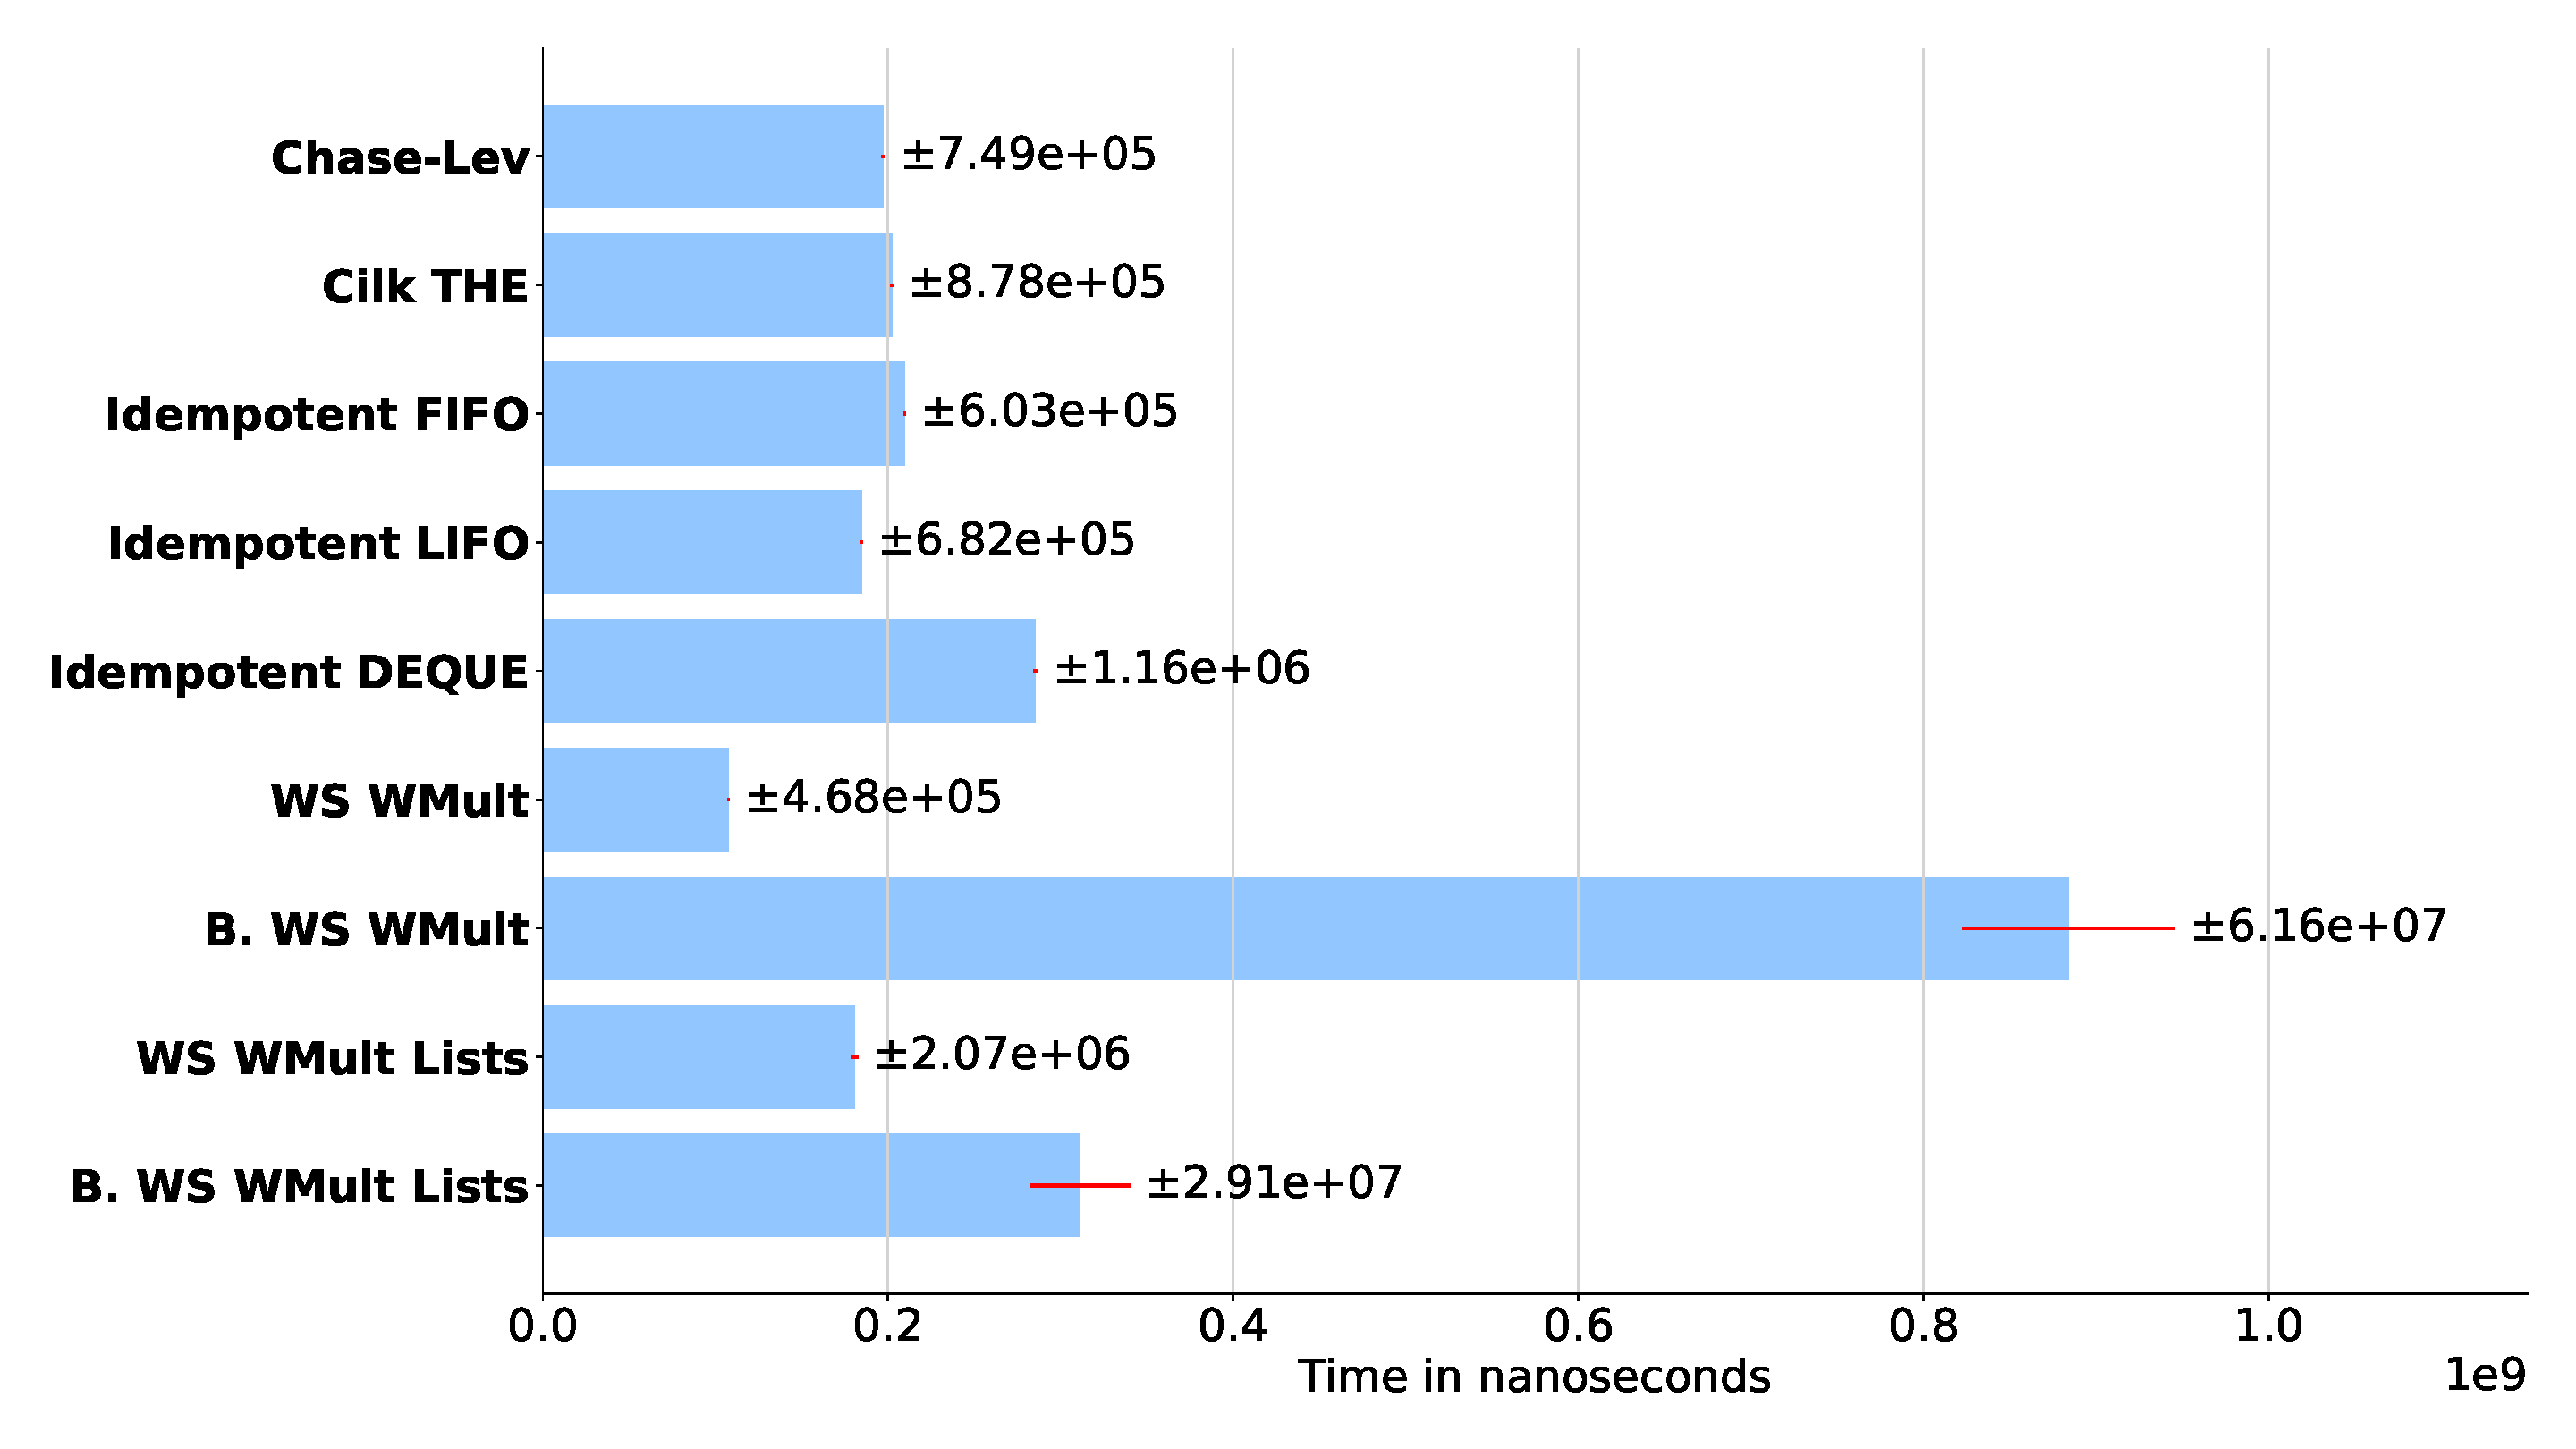
\includegraphics[width=0.47\textwidth]{contents/figures/IV_6_chart-puts-takes-1000000-10000000.pdf}
  }

  \subfloat[\label{fig:putstakes:10000000}Puts and Takes with an initial size 10,000,000]{
    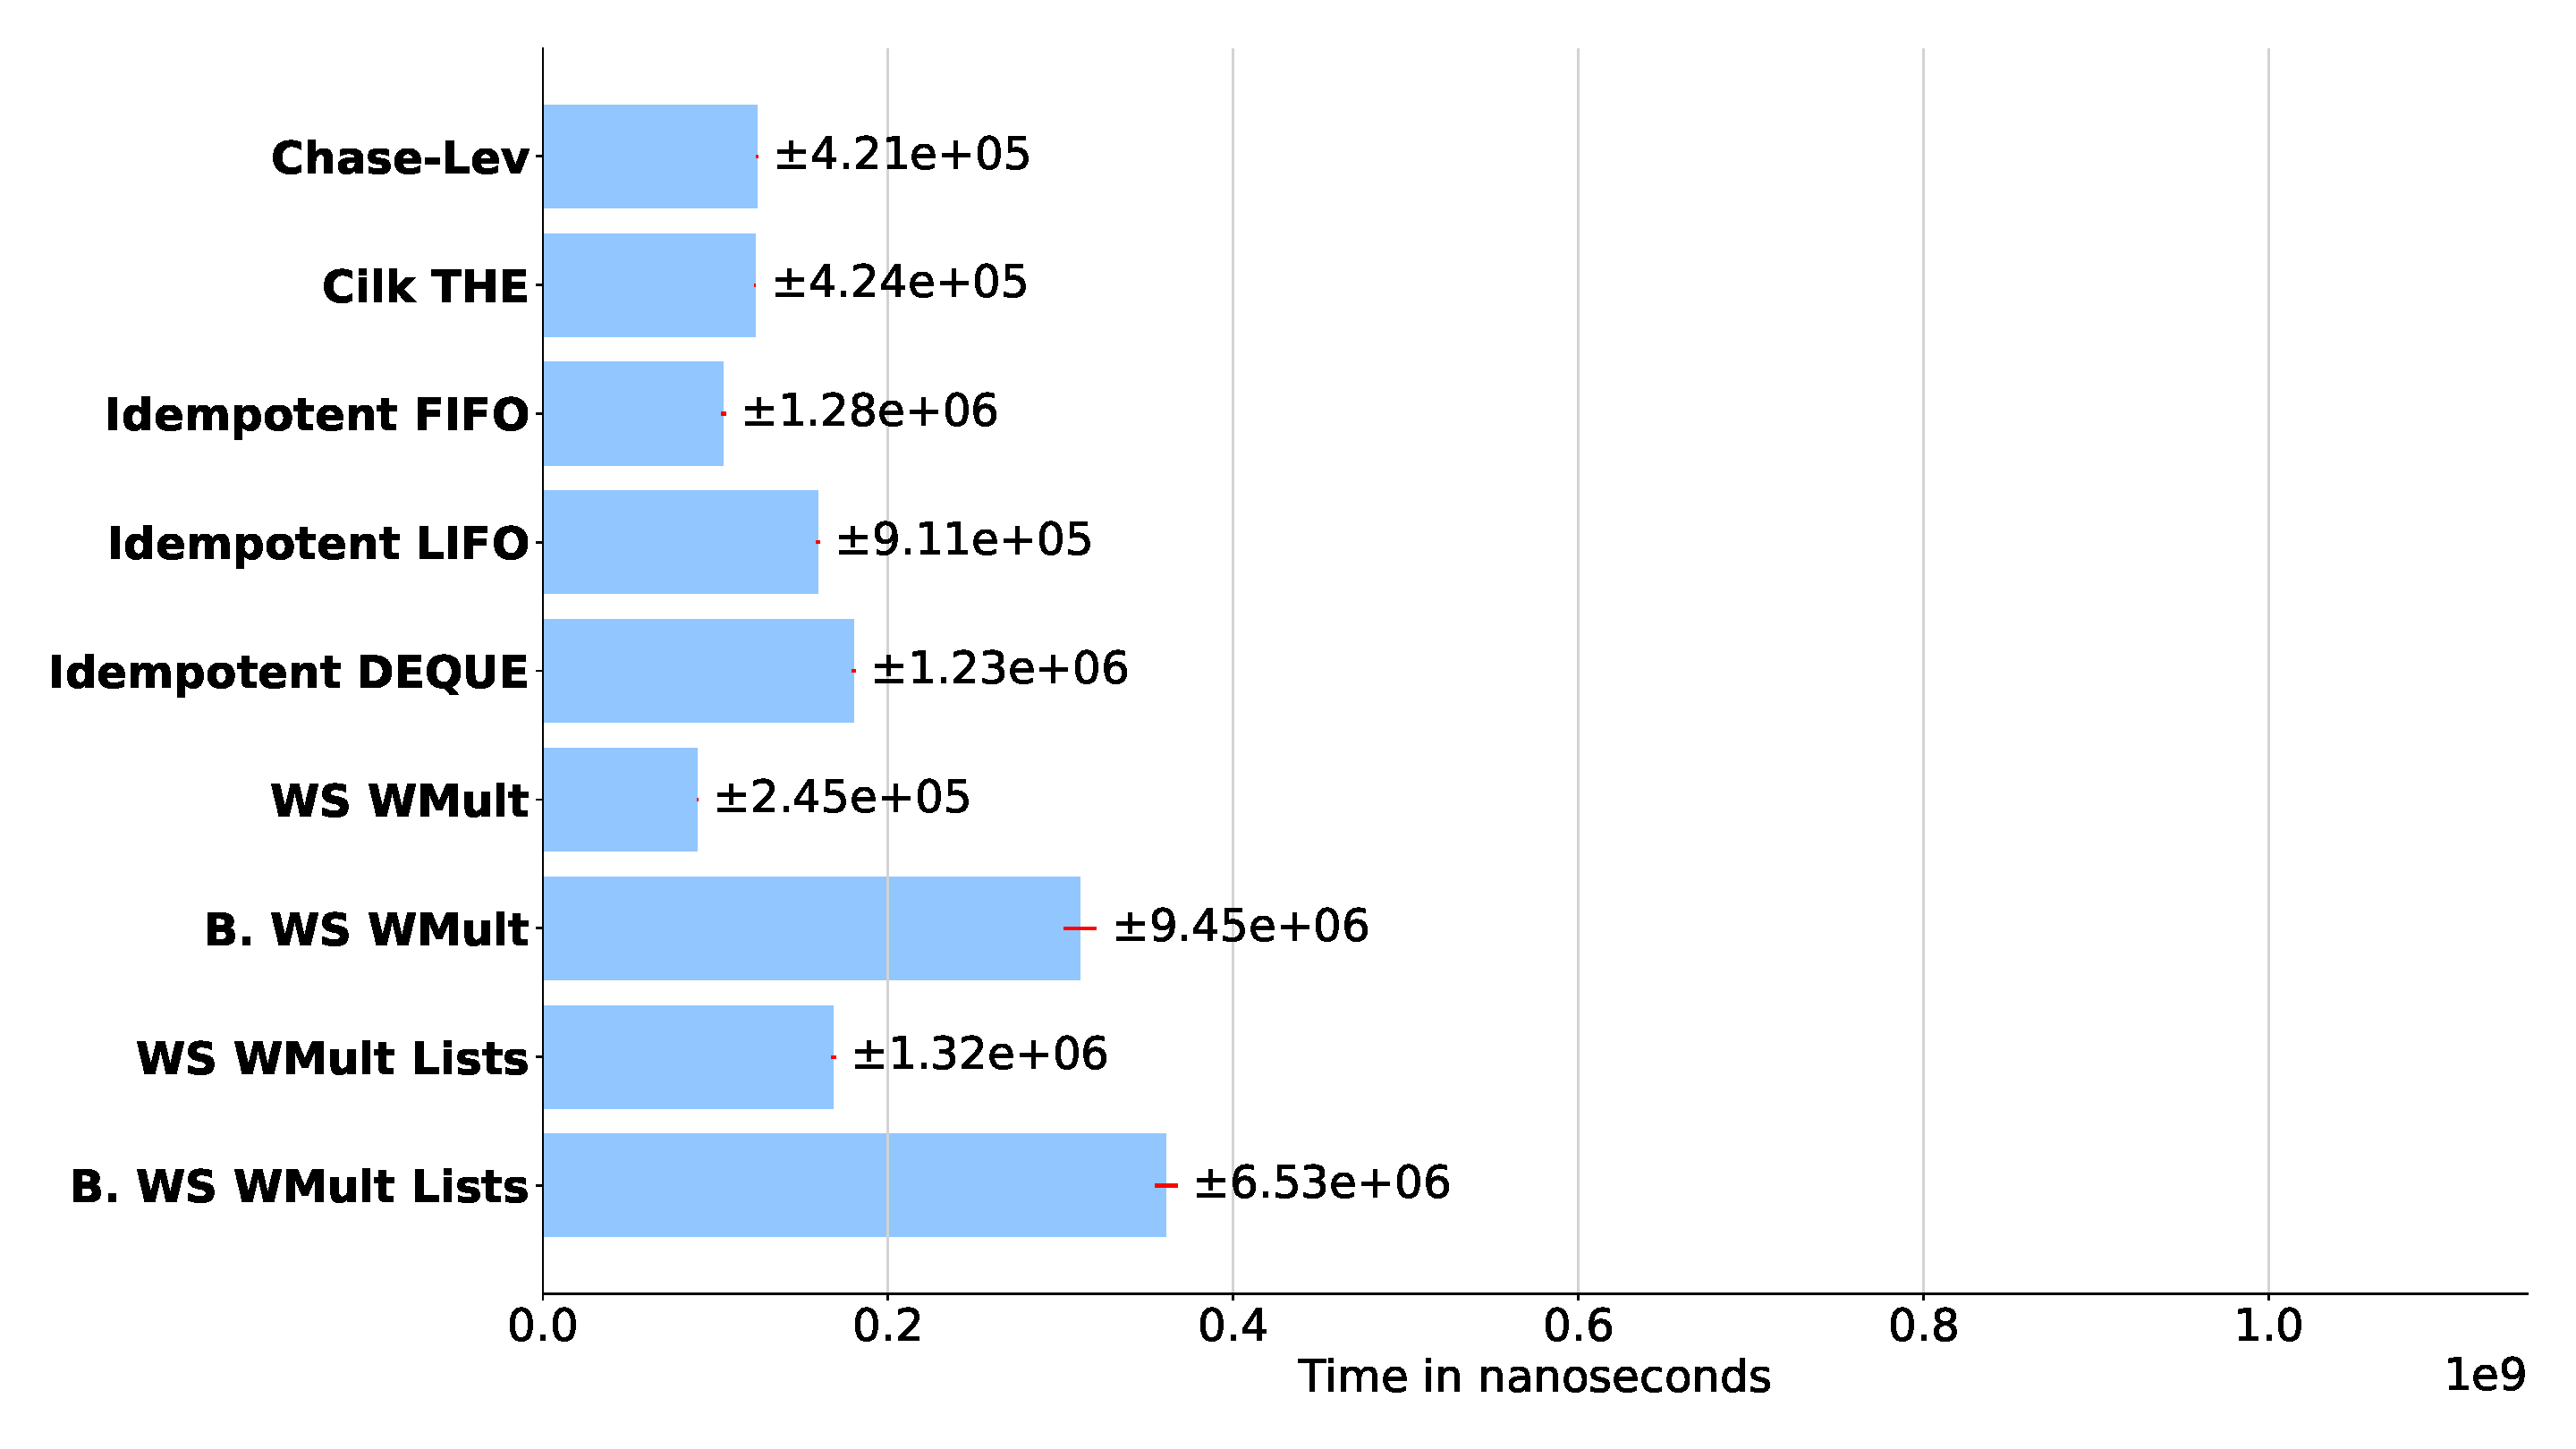
\includegraphics[width=0.47\textwidth]{contents/figures/IV_6_chart-puts-takes-10000000-10000000.pdf}
  }
  \subfloat[\label{fig:putssteals:256}Puts and Steals with an initial size 256]{
    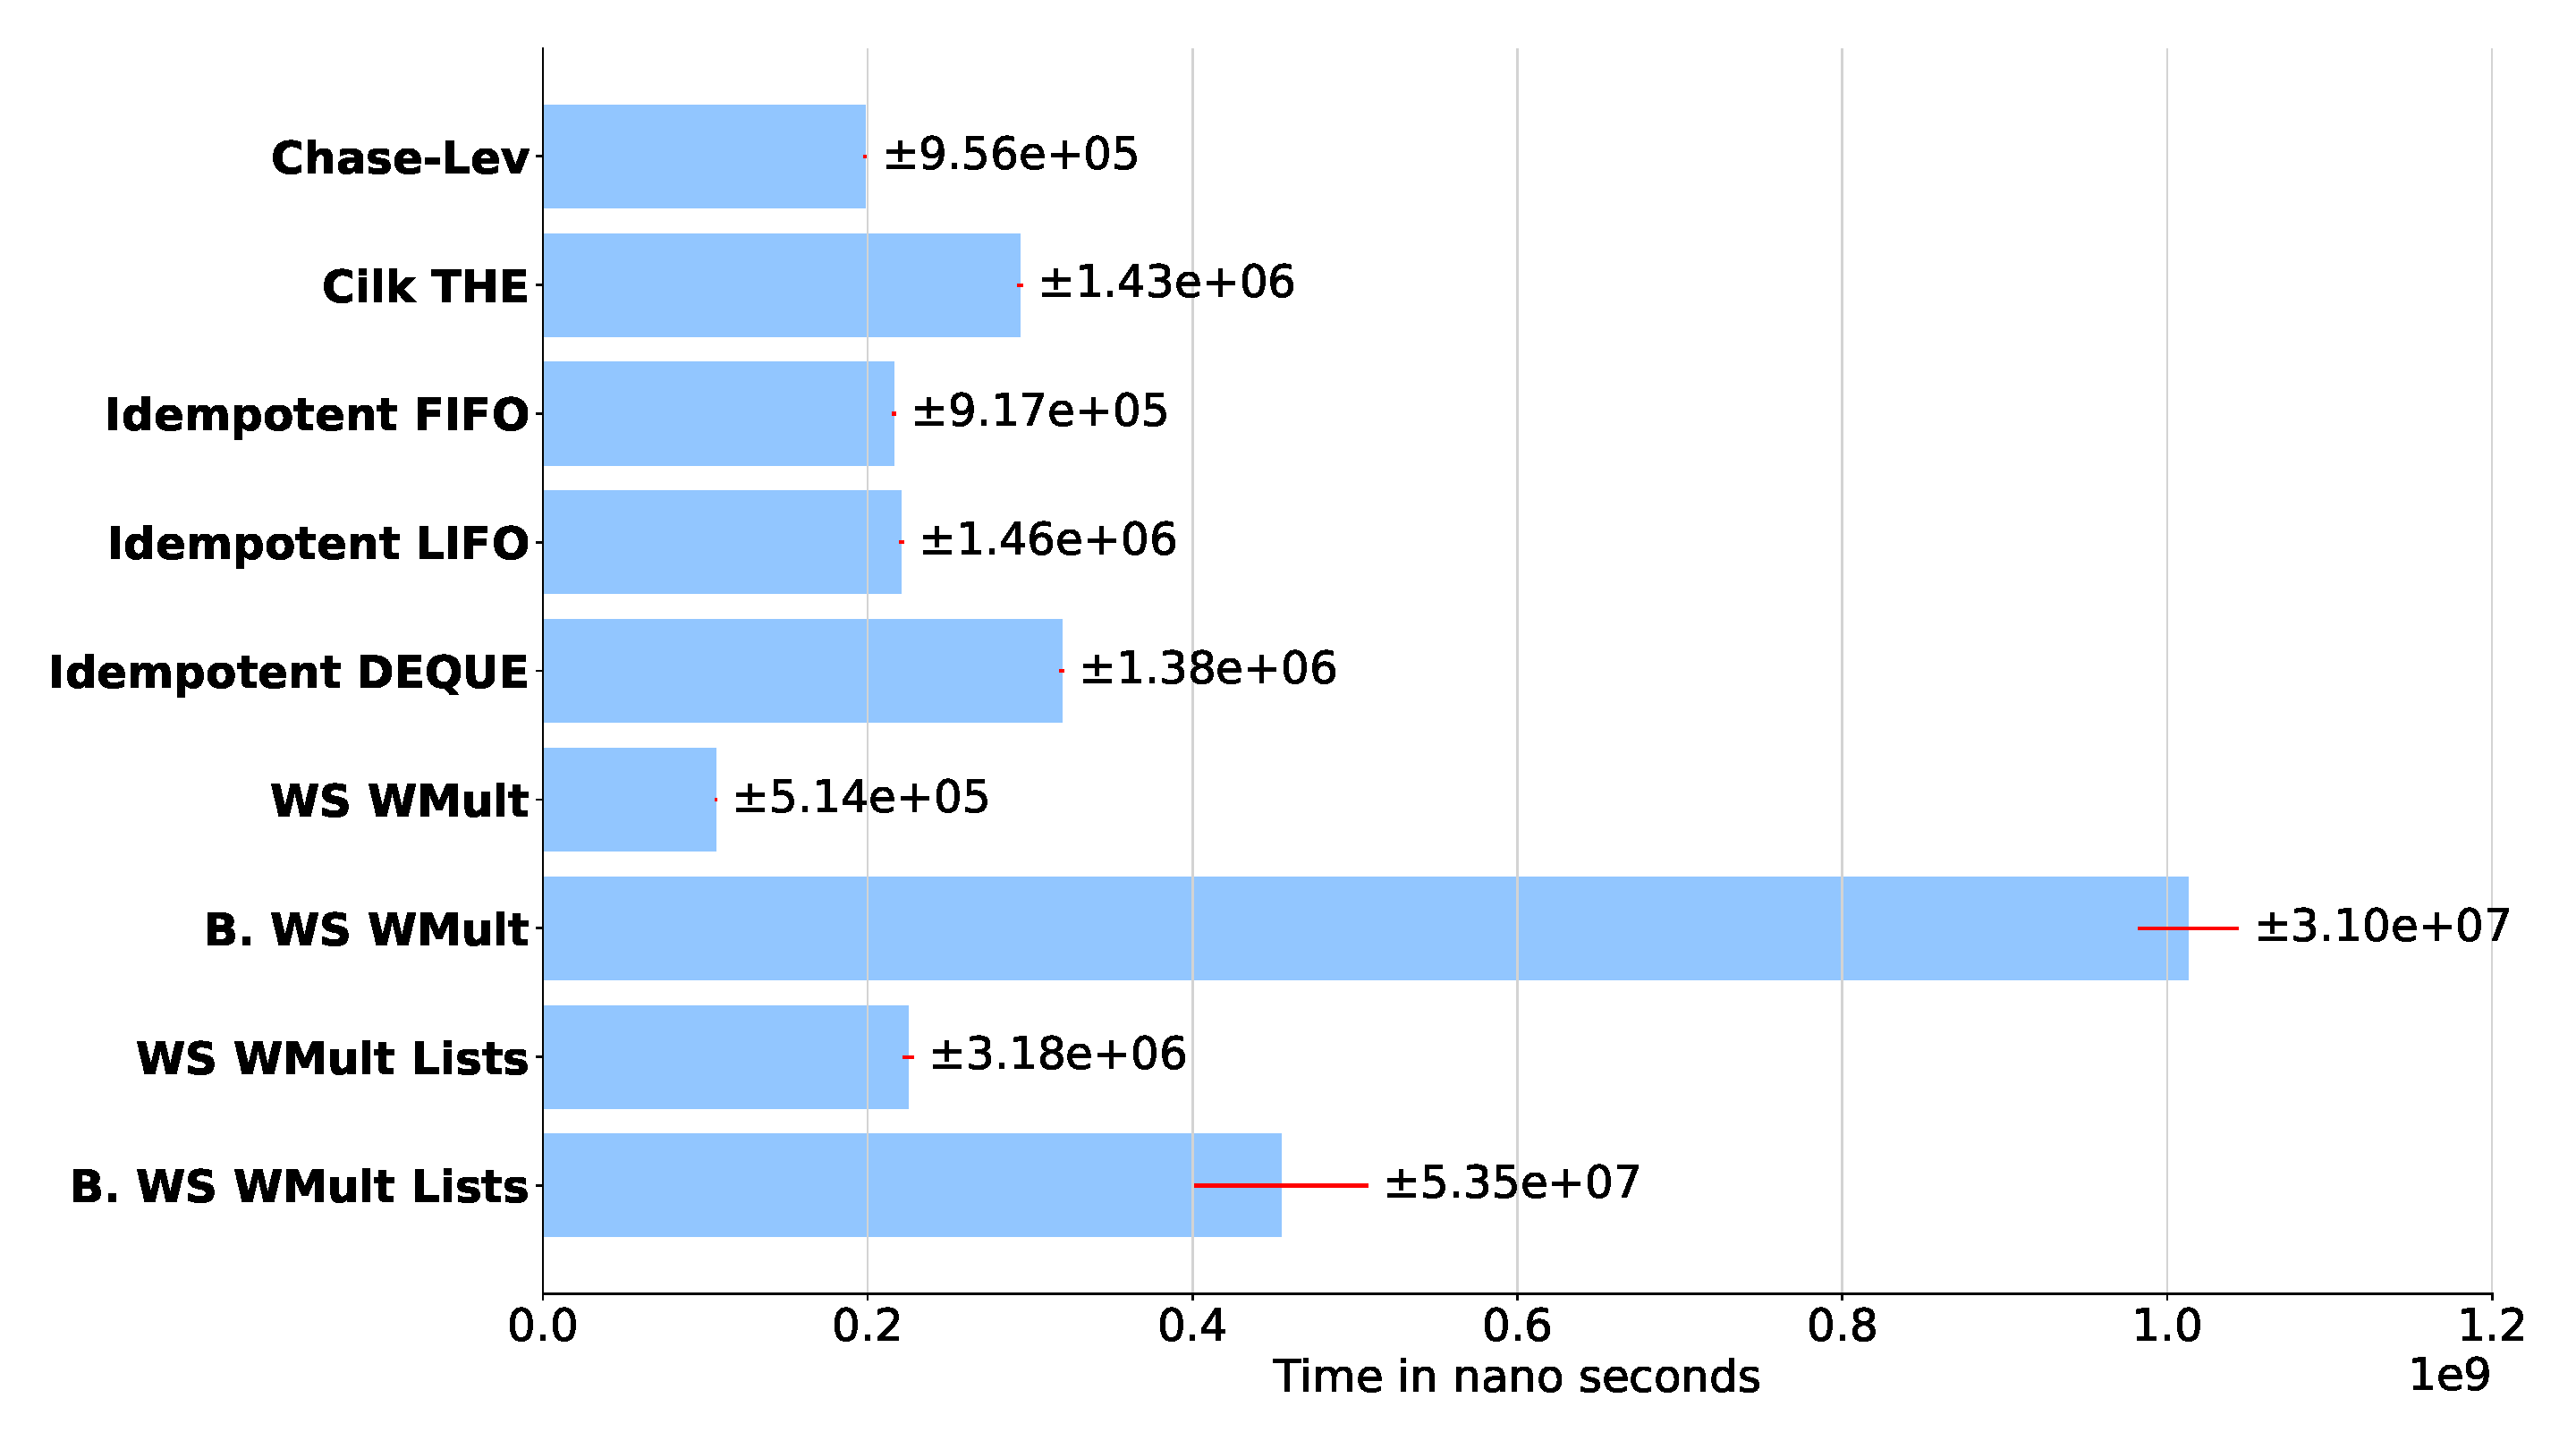
\includegraphics[width=0.47\textwidth]{contents/figures/IV_6_chart-puts-steals-256-10000000.pdf}
  }

  \subfloat[\label{fig:putssteals:1000000}Puts and Steals with an initial size 1,000,000]{
    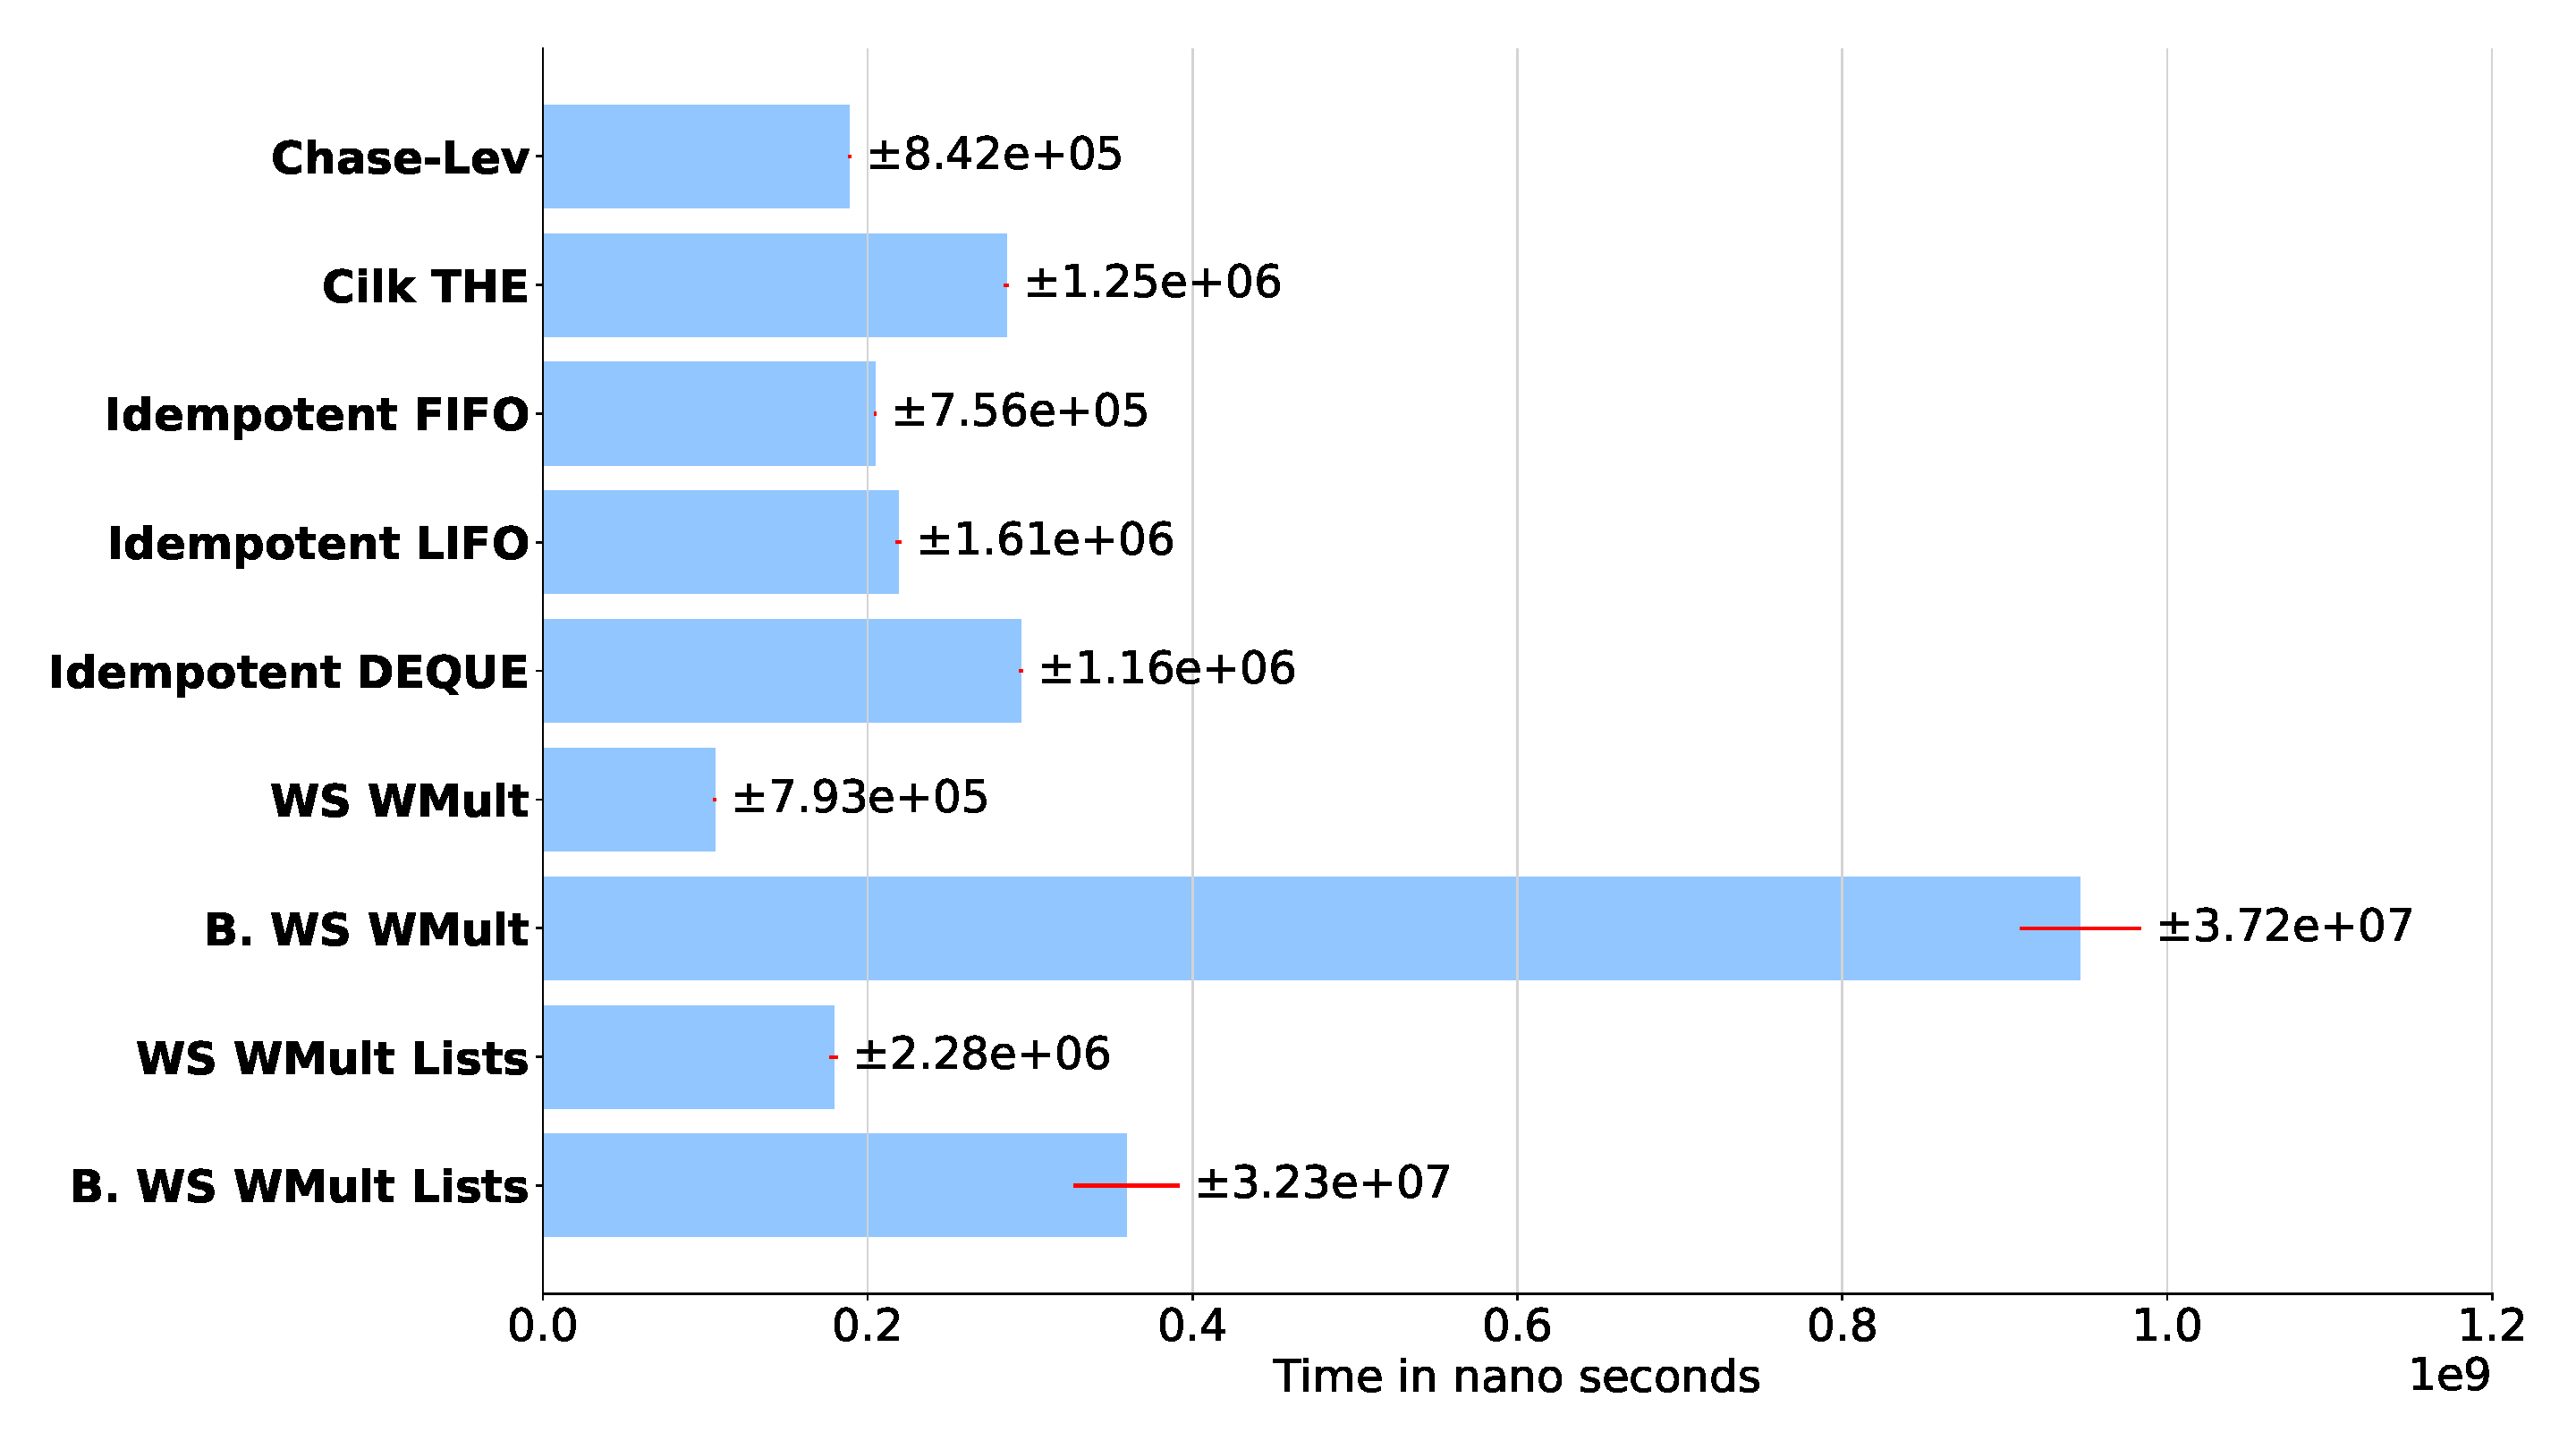
\includegraphics[width=0.47\textwidth]{contents/figures/IV_6_chart-puts-steals-1000000-10000000.pdf}

  }
  \subfloat[\label{fig:putssteals:10000000}Puts and Steals with an initial size 10,000,000]{
    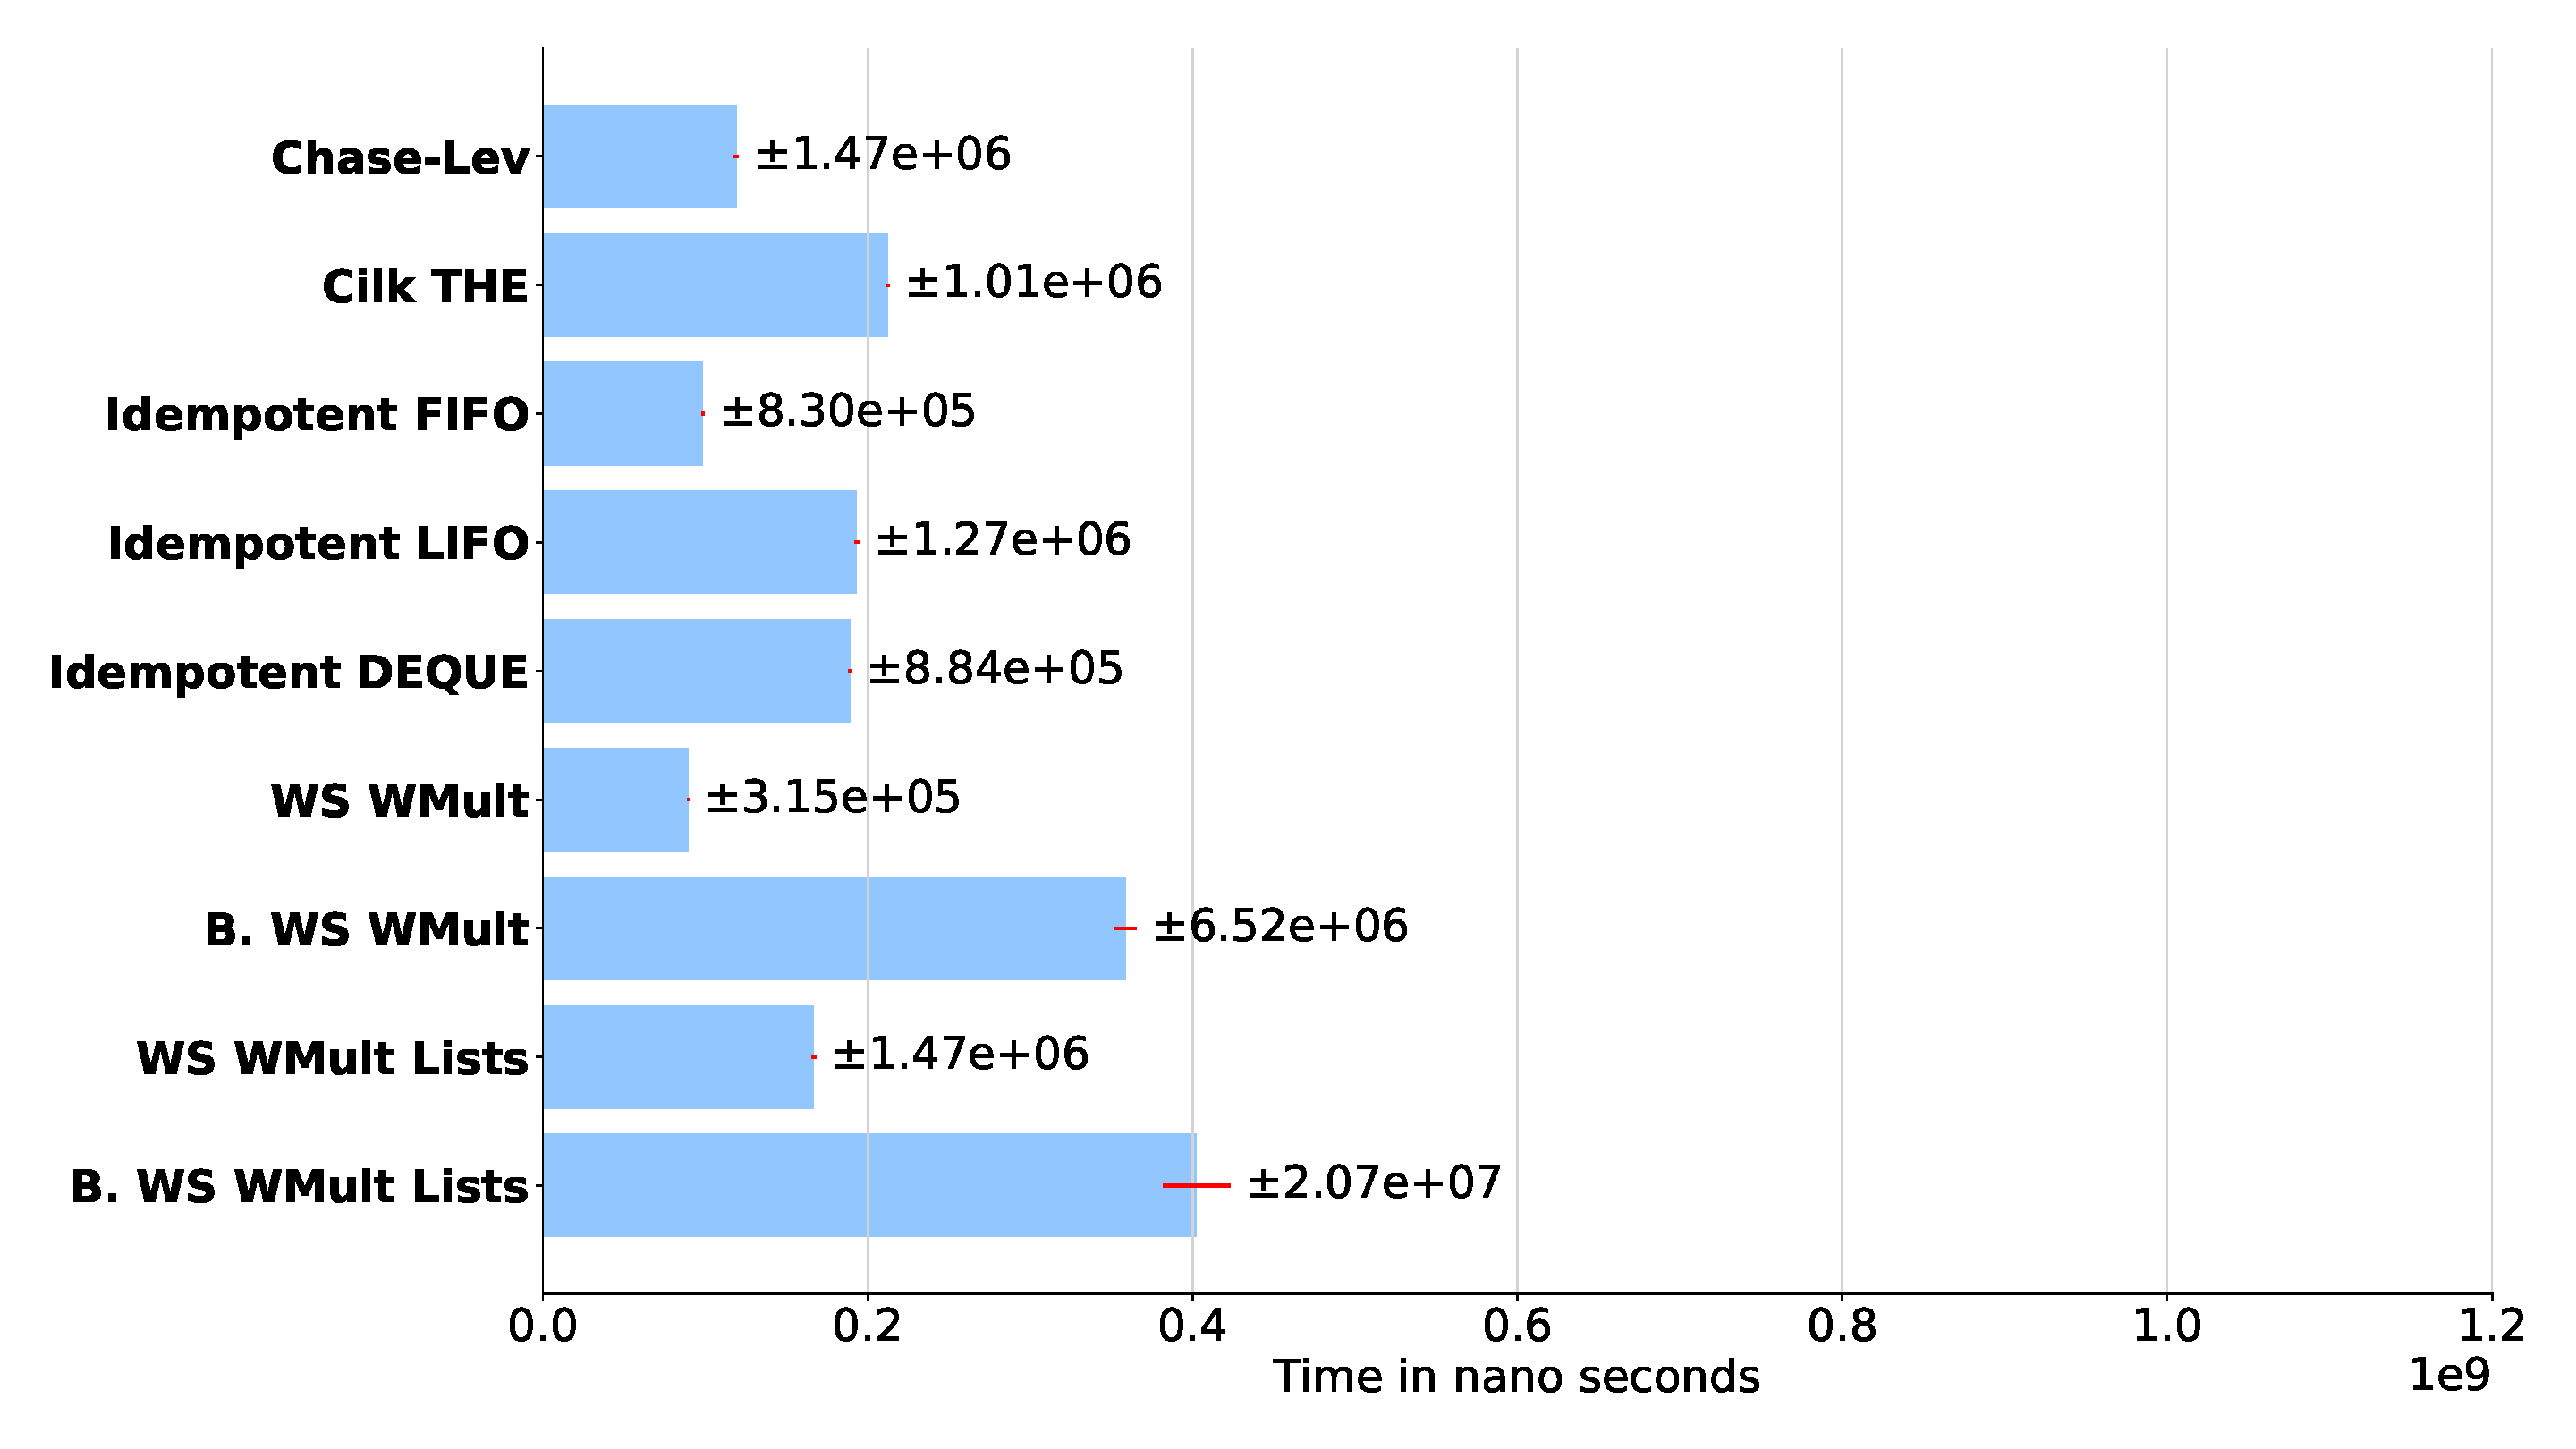
\includegraphics[width=0.4\textwidth]{contents/figures/IV_6_chart-puts-steals-10000000-10000000.pdf}
  }

  \caption{\label{fig:zerocost} Outcome of the zero cost experiments. Time is in nanoseconds, and red lines over bars show confidence intervals. The results of the $\Puts$-$\Takes$ experiment are shown in the first three charts and the results of the $\Puts$-$\Steals$ experiment are shown in the remaining charts.}

\end{figure}


\subsection{Parallel Spanning Tree}


Except for the case of Random graphs, where practically all algorithms performed equally, in general, \NCWSM{} outperformed all algorithms.  \NCWSM Lists and idempotent FIFO overall performed second and third best. The improvement of \NCWSM{} over \NCWSM Lists and idempotent FIFO was small, between 0.5\% and 4\%, depending on the graph. Thus, the absence of fences in \NCWSM{} resulted in a minor improvement over idempotent FIFO. It merits mentioning that \BNCWSM and its lists-based version generally showed a competitive performance, in some cases close to the first three algorithms. Usually, Cilk THE and Chase-Lev performed worst, which is expected as they use costly synchronization mechanisms, although this is not the only factor (more on this below).  \NCWSM outperformed Cilk THE by a margin between $1\%$ and $21\%$, and Chase-Lev by a margin between $0.14\%$ and $32\%$.  The lowest margins occurred in the case of Random graphs, where, as mentioned, all algorithms performed almost equally. Figure~\ref{fig:graphapplication} depicts the result of the experiment in some representative cases. In a few cases (e.g., Directed 2D Torus), Chase-Lev, Cilk THE, and idempotent LIFO performed best with few processes. This seems to be related to the topology of the graph and the insert/extract task policy of the algorithms (the owner follows LIFO).

\begin{figure}[!ht]
  \subfloat[\label{fig:torus2ddirected:256}Graph: Directed Torus 2D. Initial size of 256 items]{
    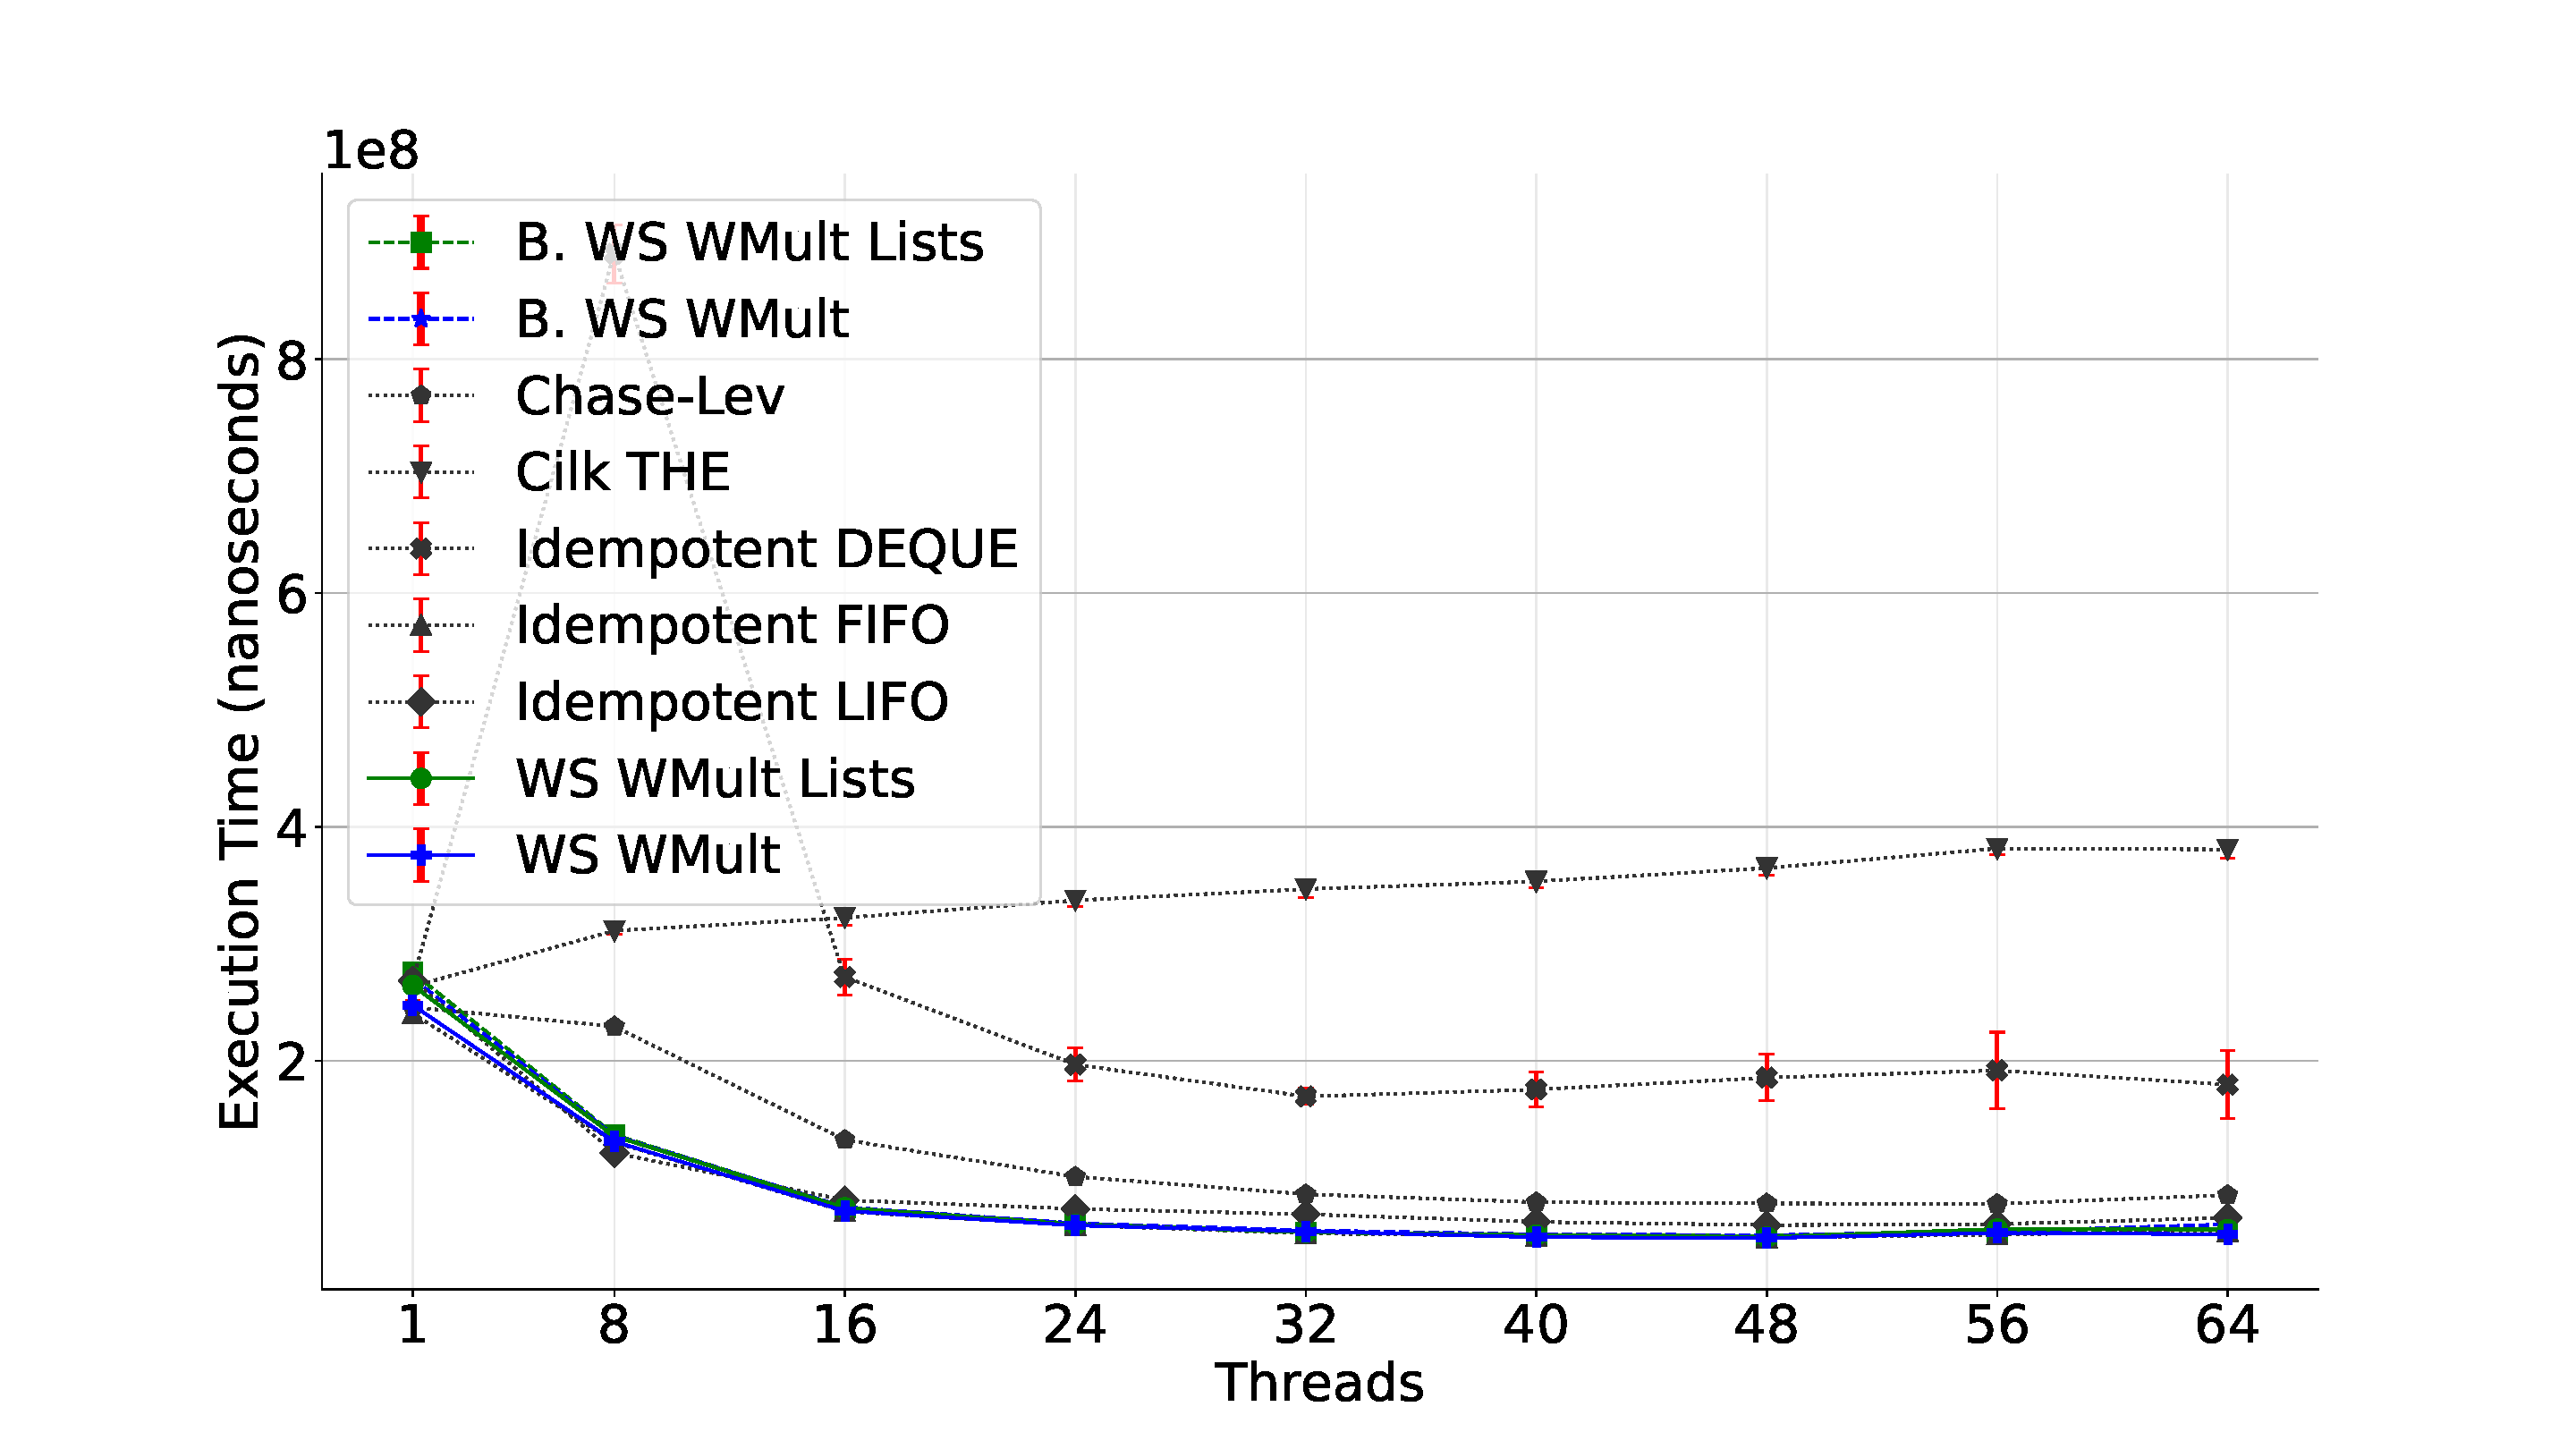
\includegraphics[width=0.48\textwidth]{contents/figures/IV_6_mean-TORUS2D-Directed-256.pdf}
  }
  \subfloat[\label{fig:torus2ddirected:1000000}Graph: Directed Torus 2D. Initial size of 1,000,000 items]{
    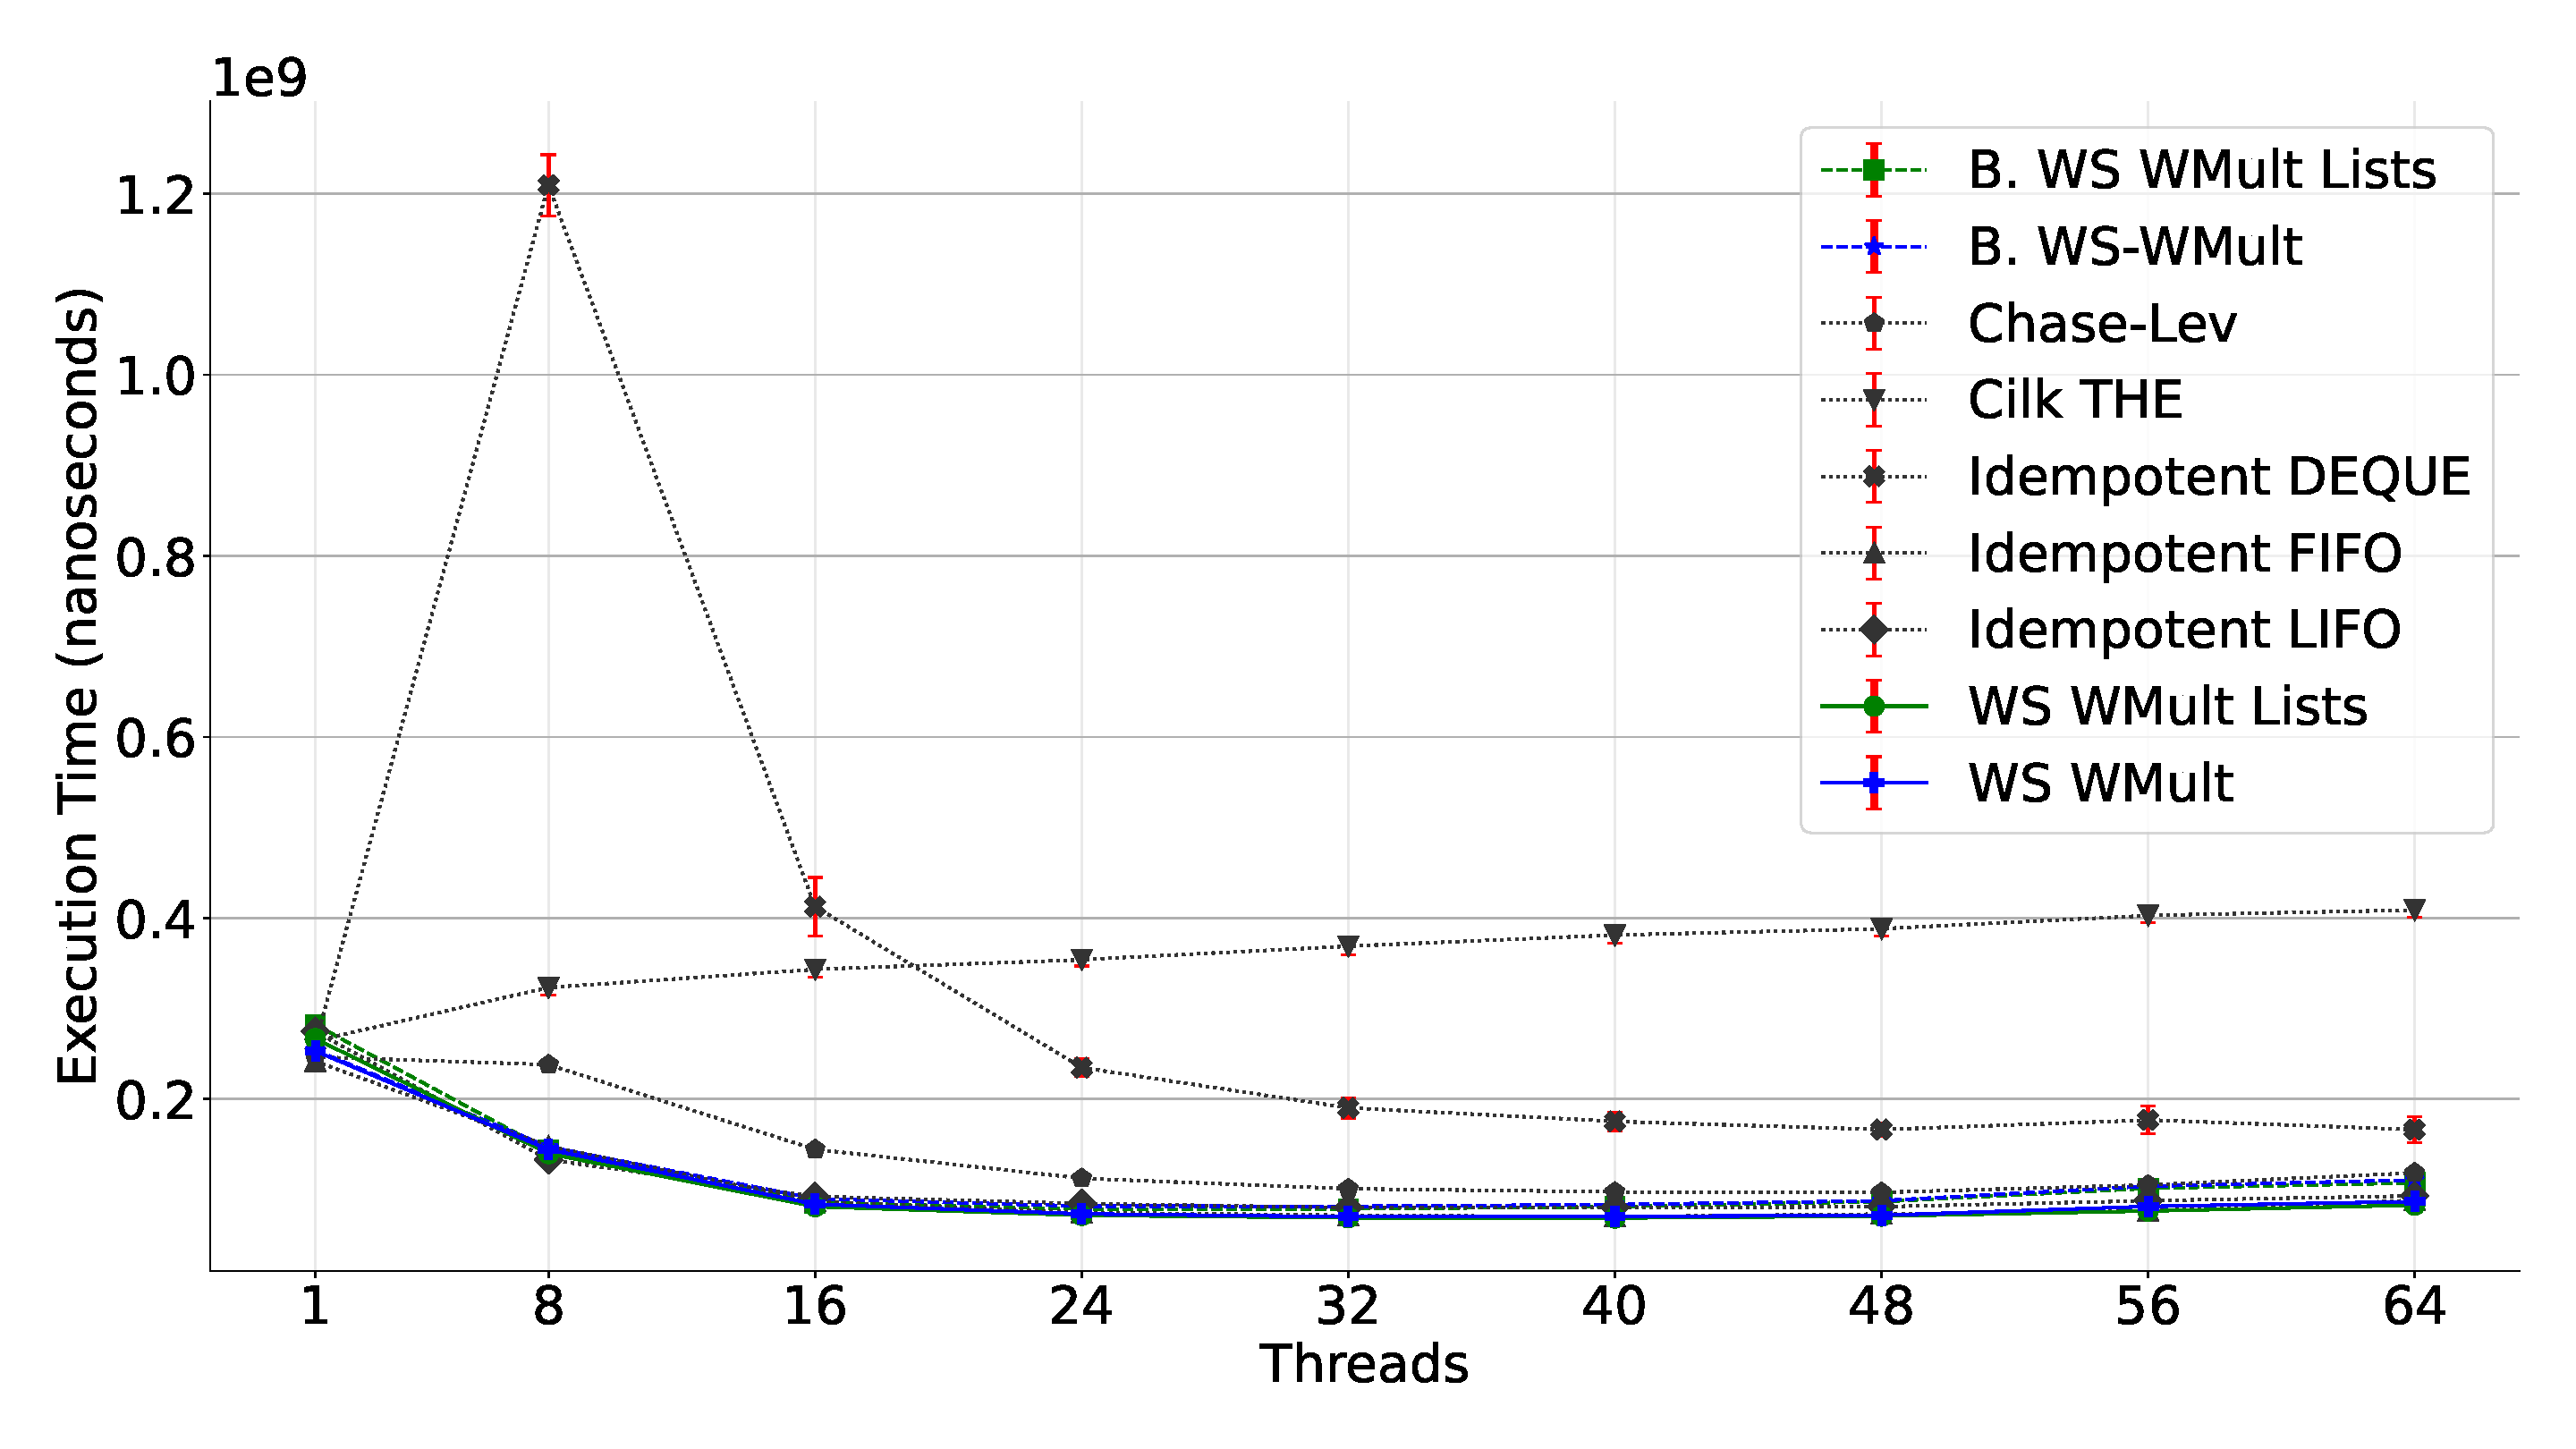
\includegraphics[width=0.48\textwidth]{contents/figures/IV_6_mean-TORUS2D-Directed-1000000.pdf}
  }

  \subfloat[\label{fig:torus3ddirected:256}Graph: Directed Torus 3D. Initial size of 256 items]{
    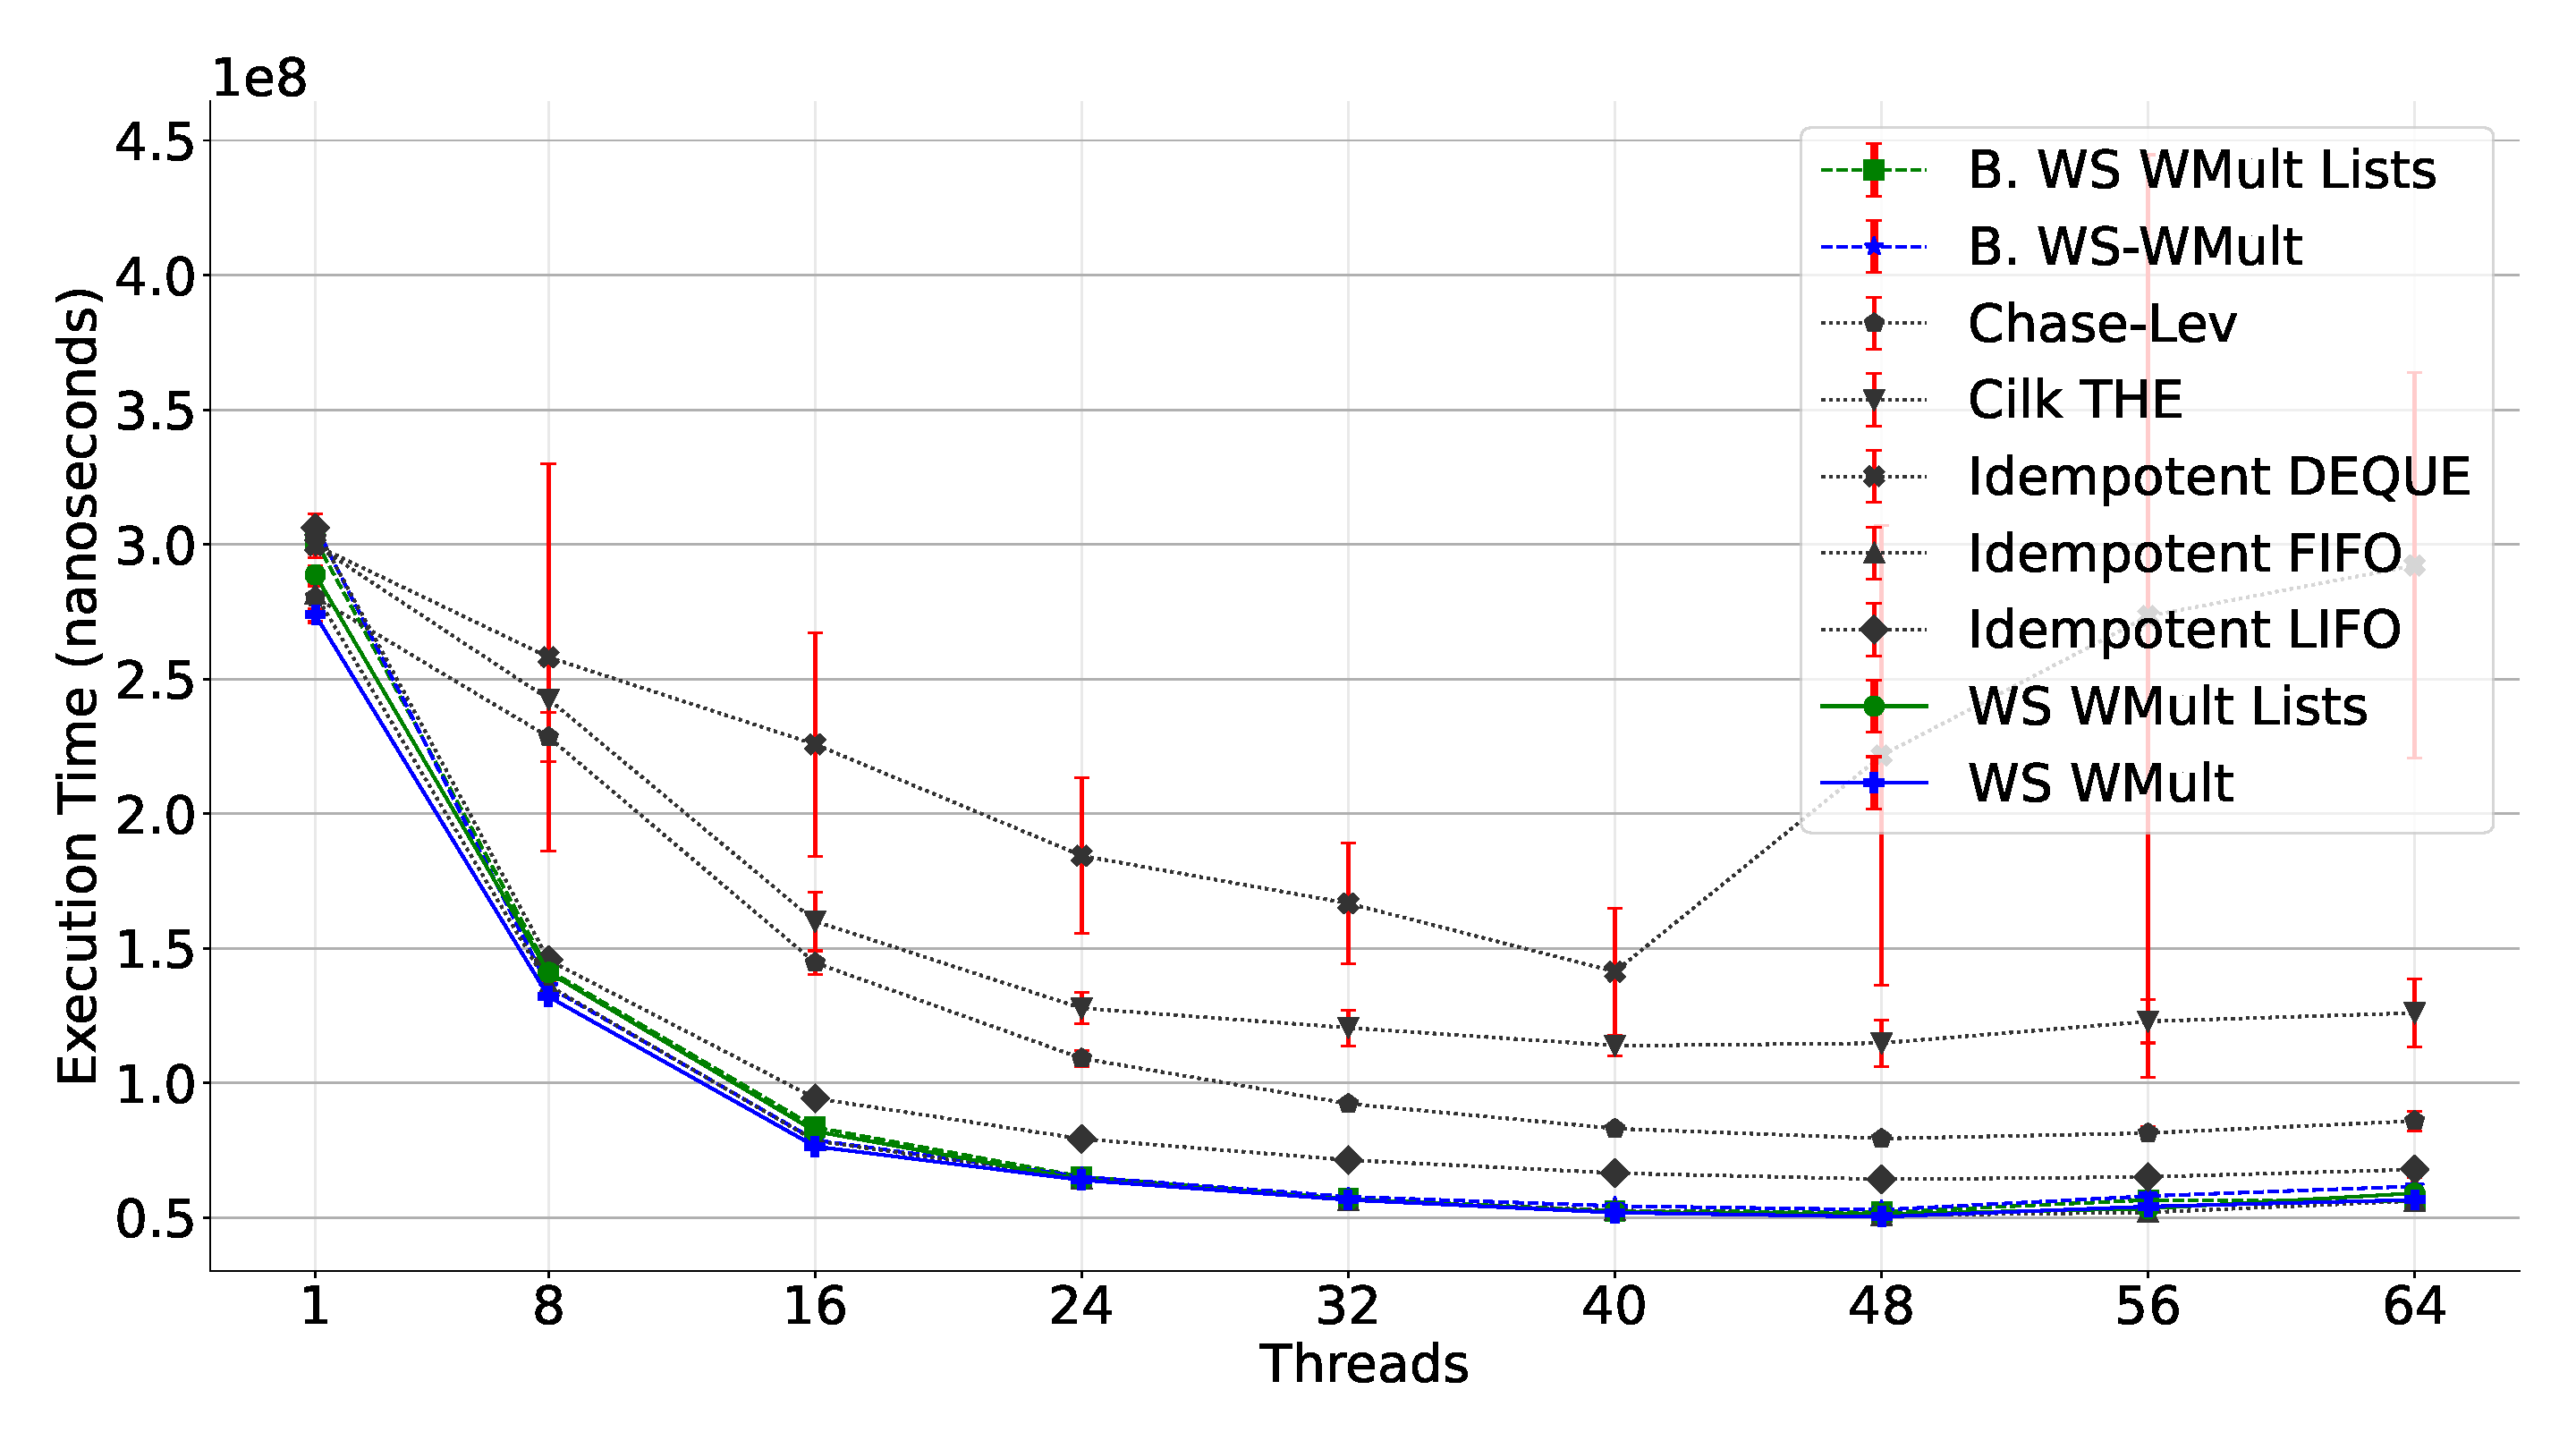
\includegraphics[width=0.48\textwidth]{contents/figures/IV_6_mean-TORUS3D-Directed-256.pdf}
  }
  \subfloat[\label{fig:torus3ddirected:1000000}Graph: Directed Torus 3D. Initial size of 1,000,000 items]{
    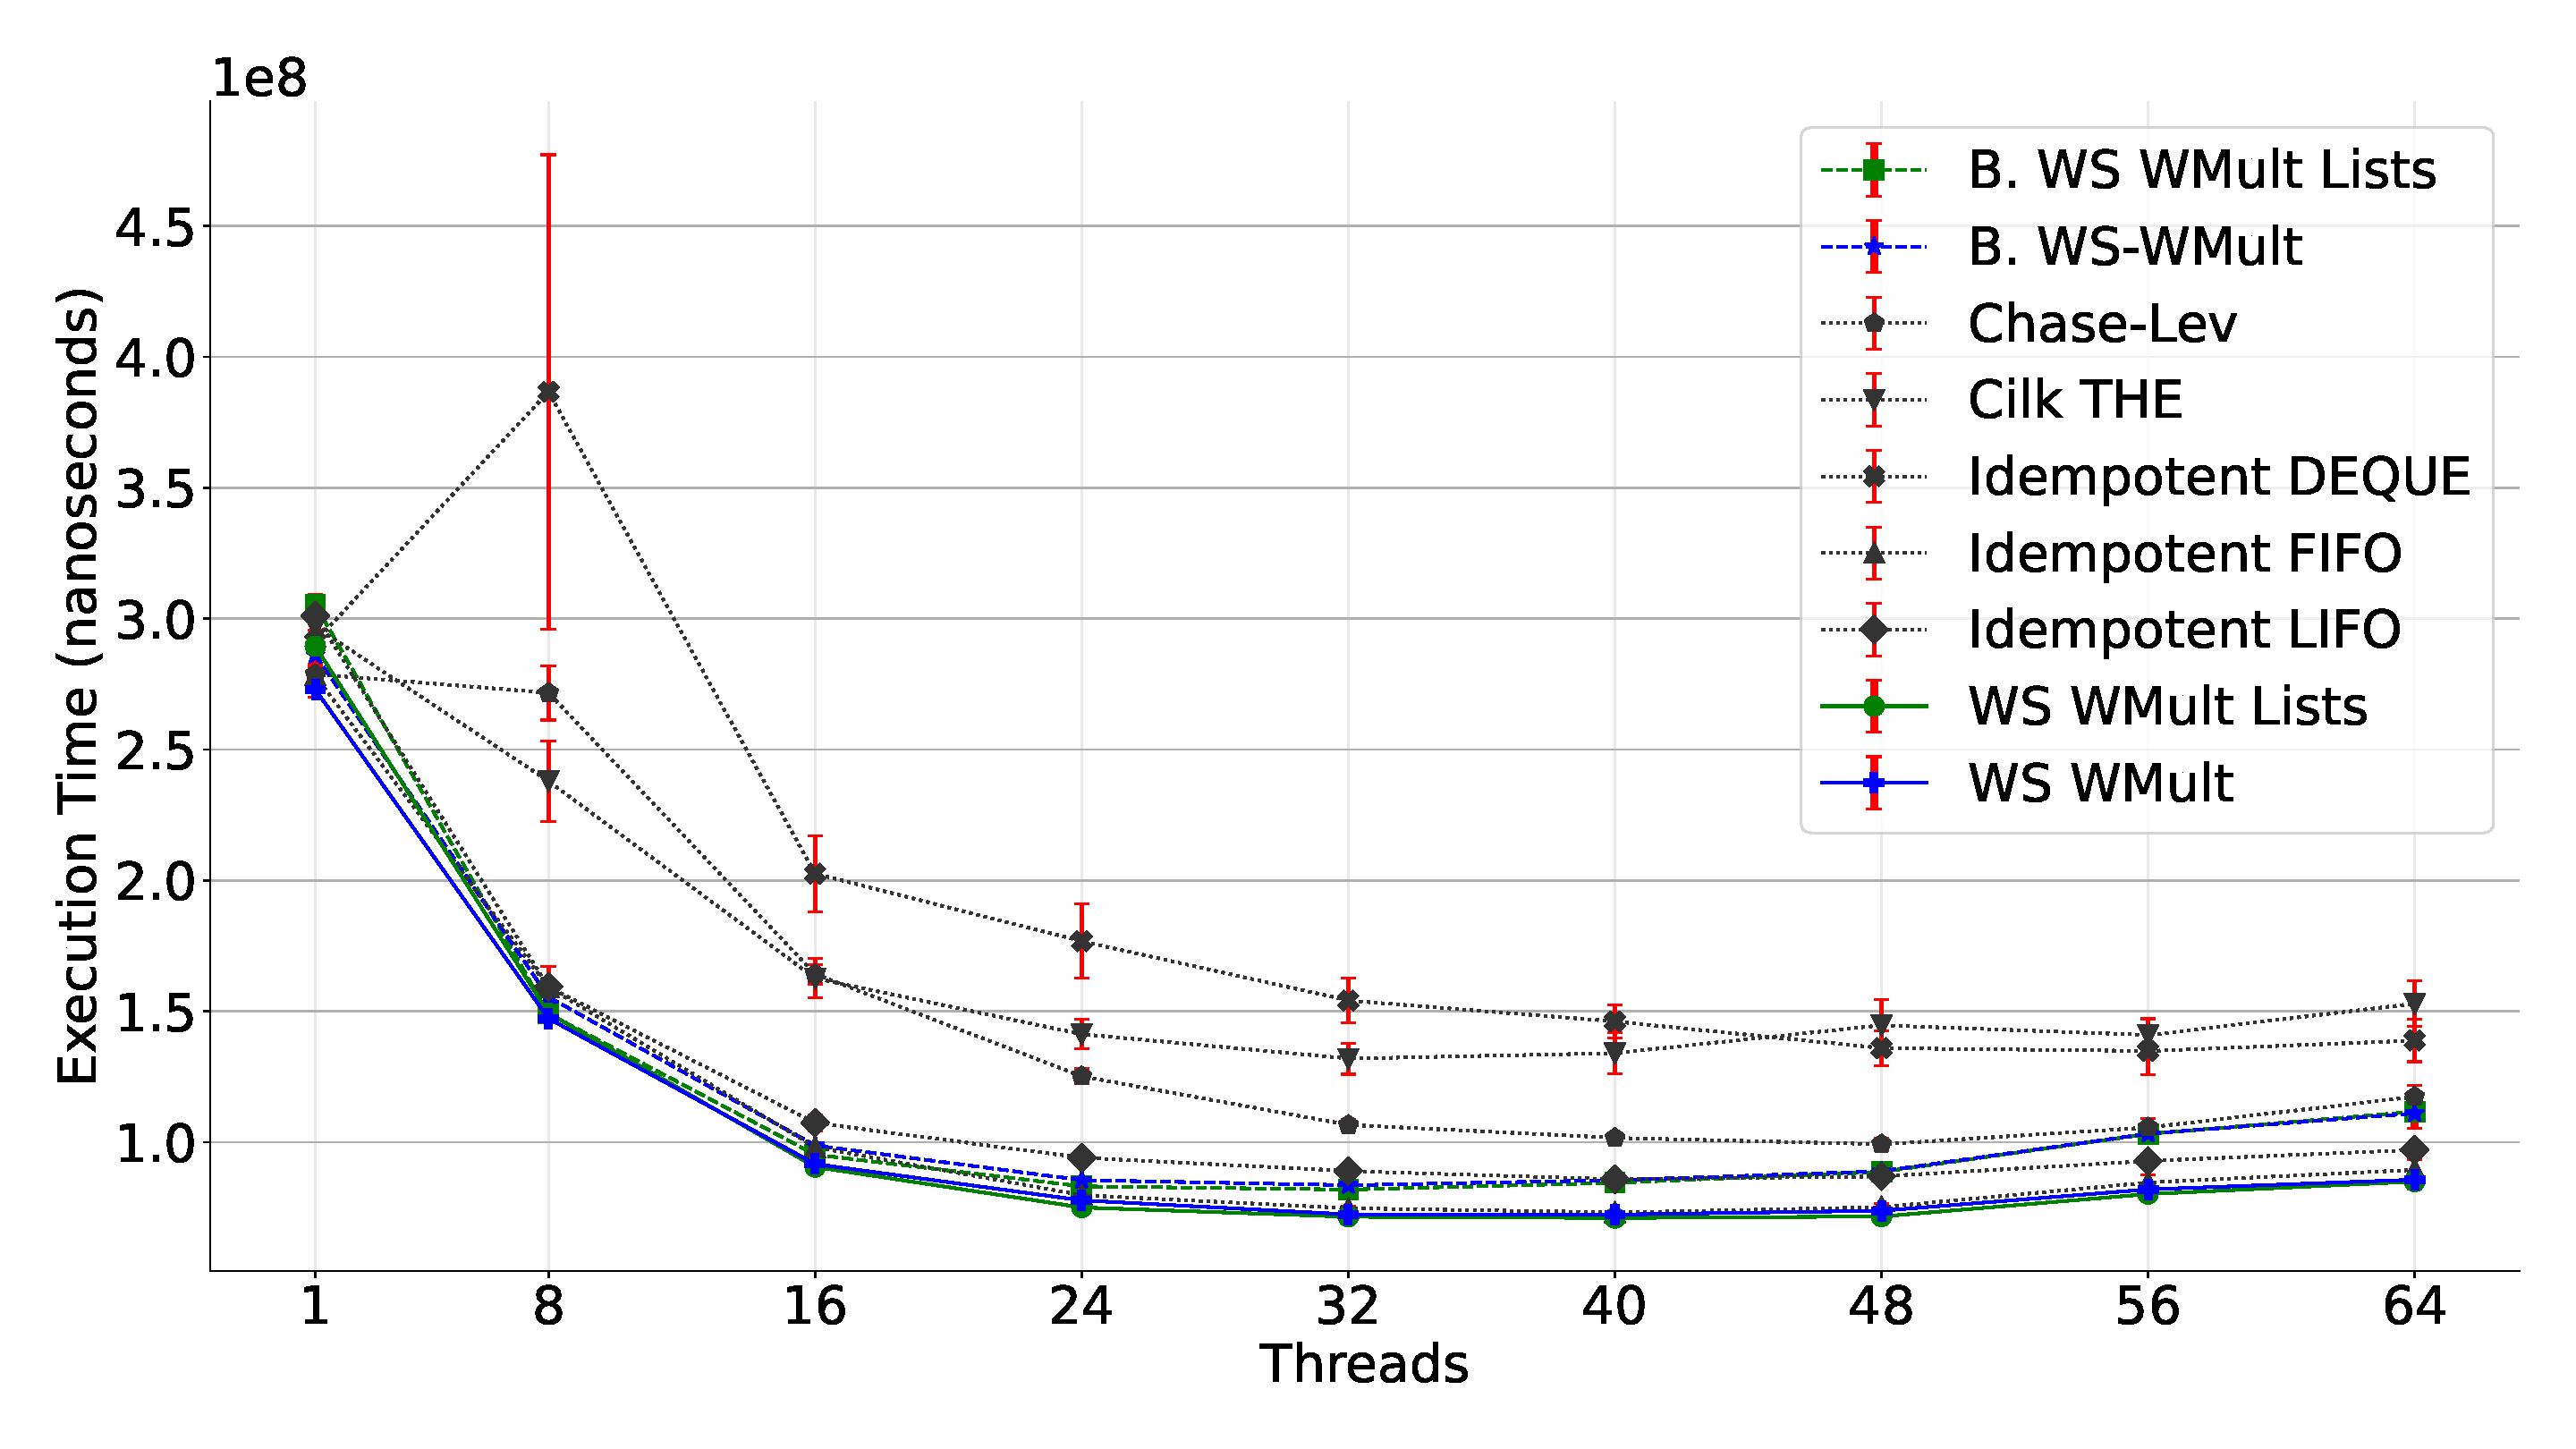
\includegraphics[width=0.48\textwidth]{contents/figures/IV_6_mean-TORUS3D-Directed-1000000.pdf}
  }

  \subfloat[\label{fig:random:256}Graph: Directed Random. Initial size of 256 entries]{
    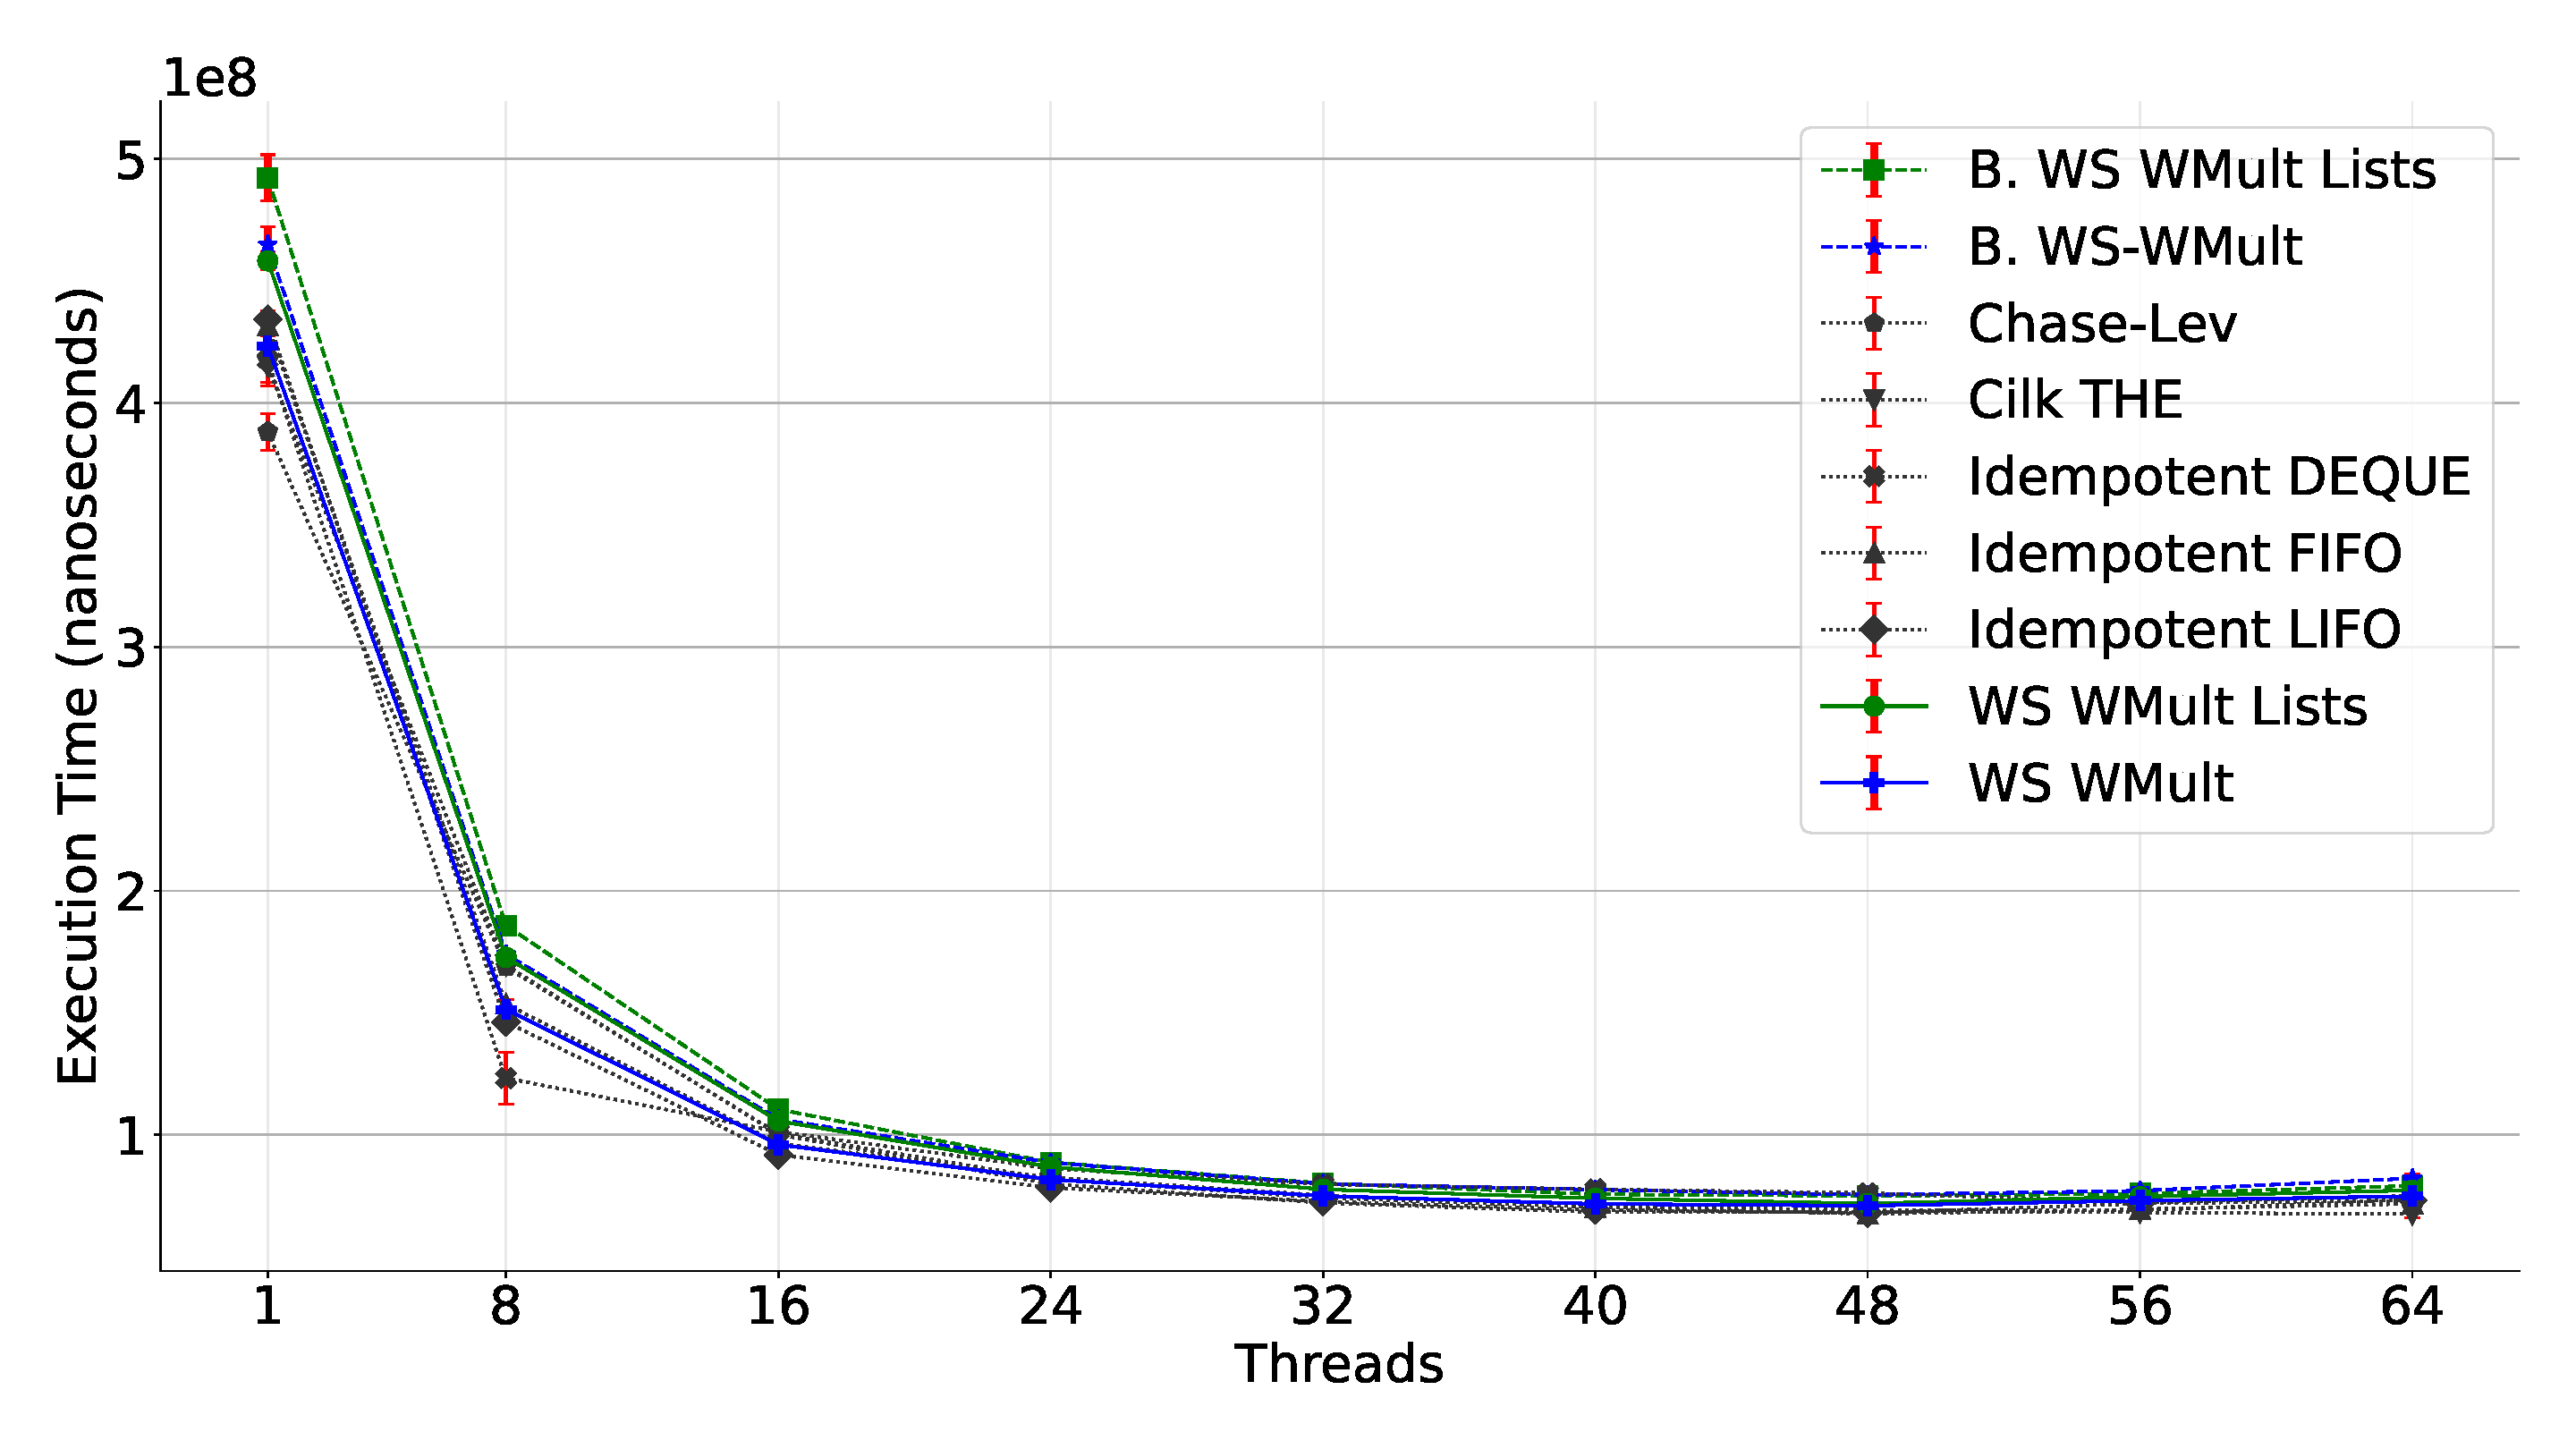
\includegraphics[width=0.48\textwidth]{contents/figures/IV_6_mean-RANDOM-Directed-256.pdf}
  }
  \subfloat[\label{fig:random:1000000}Graph: Directed Random: Initial size of 1,000,000 entries]{
    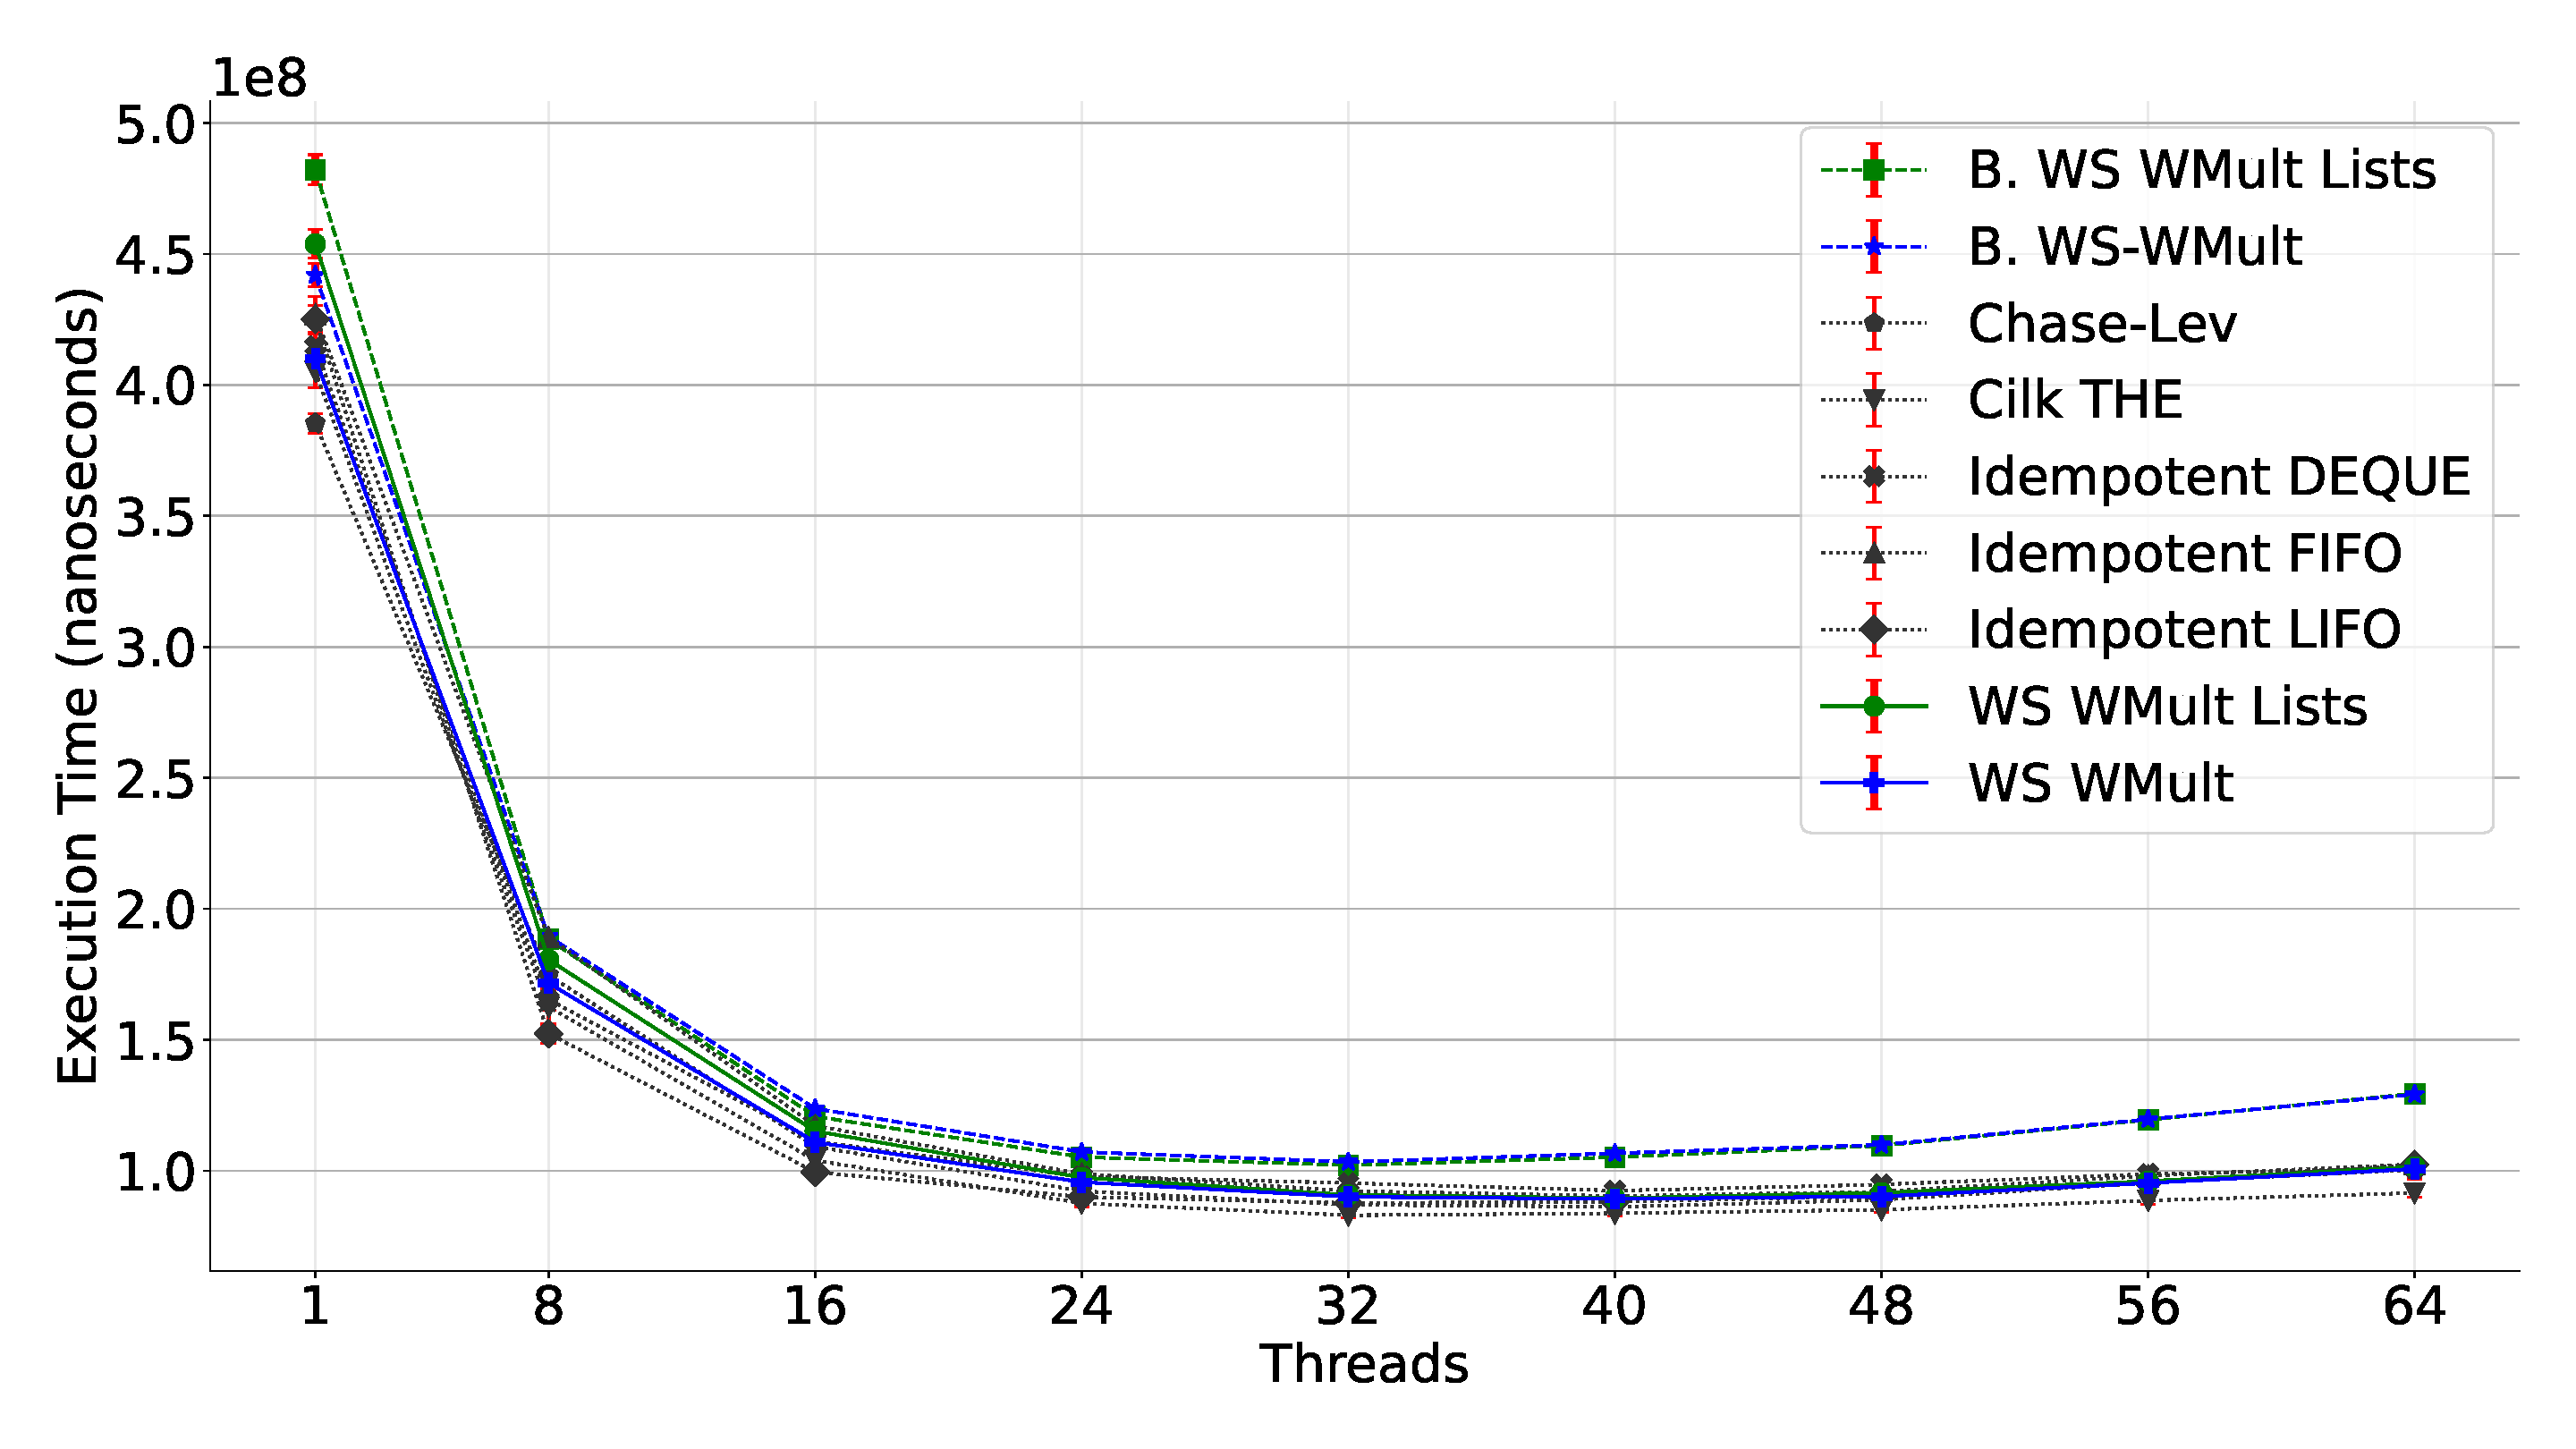
\includegraphics[width=0.48\textwidth]{contents/figures/IV_6_mean-RANDOM-Directed-1000000.pdf}
  }

  \caption{\label{fig:graphapplication} Mean times reported for executing the graph application benchmark.}
\end{figure}

Repeated work was measured indirectly through the total number of \Puts (work to be executed), which was compared to the total number of \Puts in sequential executions (i.e., $1,000,000$). The difference between these two numbers is called surplus work. Surplus work in all algorithms with FIFO insert/extract policy was generally low, less than $0.7\%$. All these algorithms implement work-stealing with relaxed semantics. Thus, even if all surplus work was due to relaxation (recall that surplus work can occur even with non-relaxed work-stealing algorithms), it rarely happened, with little impact on performance. In sharp contrast, in all algorithms where the owner follows the LIFO insert/extract policy, Cilk THE, Chase-Lev, idempotent LIFO, and idempotent Deque, surplus work was at least $\bf XX\%??$, and in some cases it reached $\bf 56\%??$. Therefore, neither multiplicity nor idempotency per se increased surplus work considerably, and the dominant factor seems to be the task insert/extract policy combined with the solved problem. Figure~\ref{fig:surplusgraphapplication} depicts the surplus work of the experiments in Figure~\ref{fig:graphapplication}.

In all algorithms, not all tasks are executed. Processes are constantly checking the distinct number of vertices that have been processed so far, and when this number reaches $1,000,000$, the spanning tree is computed, and the experiment terminates. It can be the case that some vertices remain in one or more work-stealing structures when the tree is finished; hence, not necessarily all surplus work is executed. It measured the executed surplus work, i.e., the difference between the total number of \Takes (actual work performed) and the total number of \Takes in sequential executions (i.e., $1,000,000$). Surplus executed work in Cilk THE, Chase-Lev, idempotent LIFO, and idempotent Deque ranged between $\bf XX\%??$ and $\bf XX\%??$. Figure~{\bf XX??} shows the executed surplus work of the experiments in Figure~\ref{fig:graphapplication}. Finally, in some experiments (e.g., in Random graphs), \NCWSM executed more surplus work than the algorithms with LIFO insert/extract policy, but still, it performed slightly better. We attribute this to the fact that in the FIFO policy, \Takes are more likely to read tasks from cache memory, whereas in LIFO, \Takes are more likely to read from main memory, which is costly.


\begin{figure}
  \subfloat[\label{fig:surplustorus2ddirected:256}Surplus work: Directed Torus 2D. Initial size of 256 items.]{
    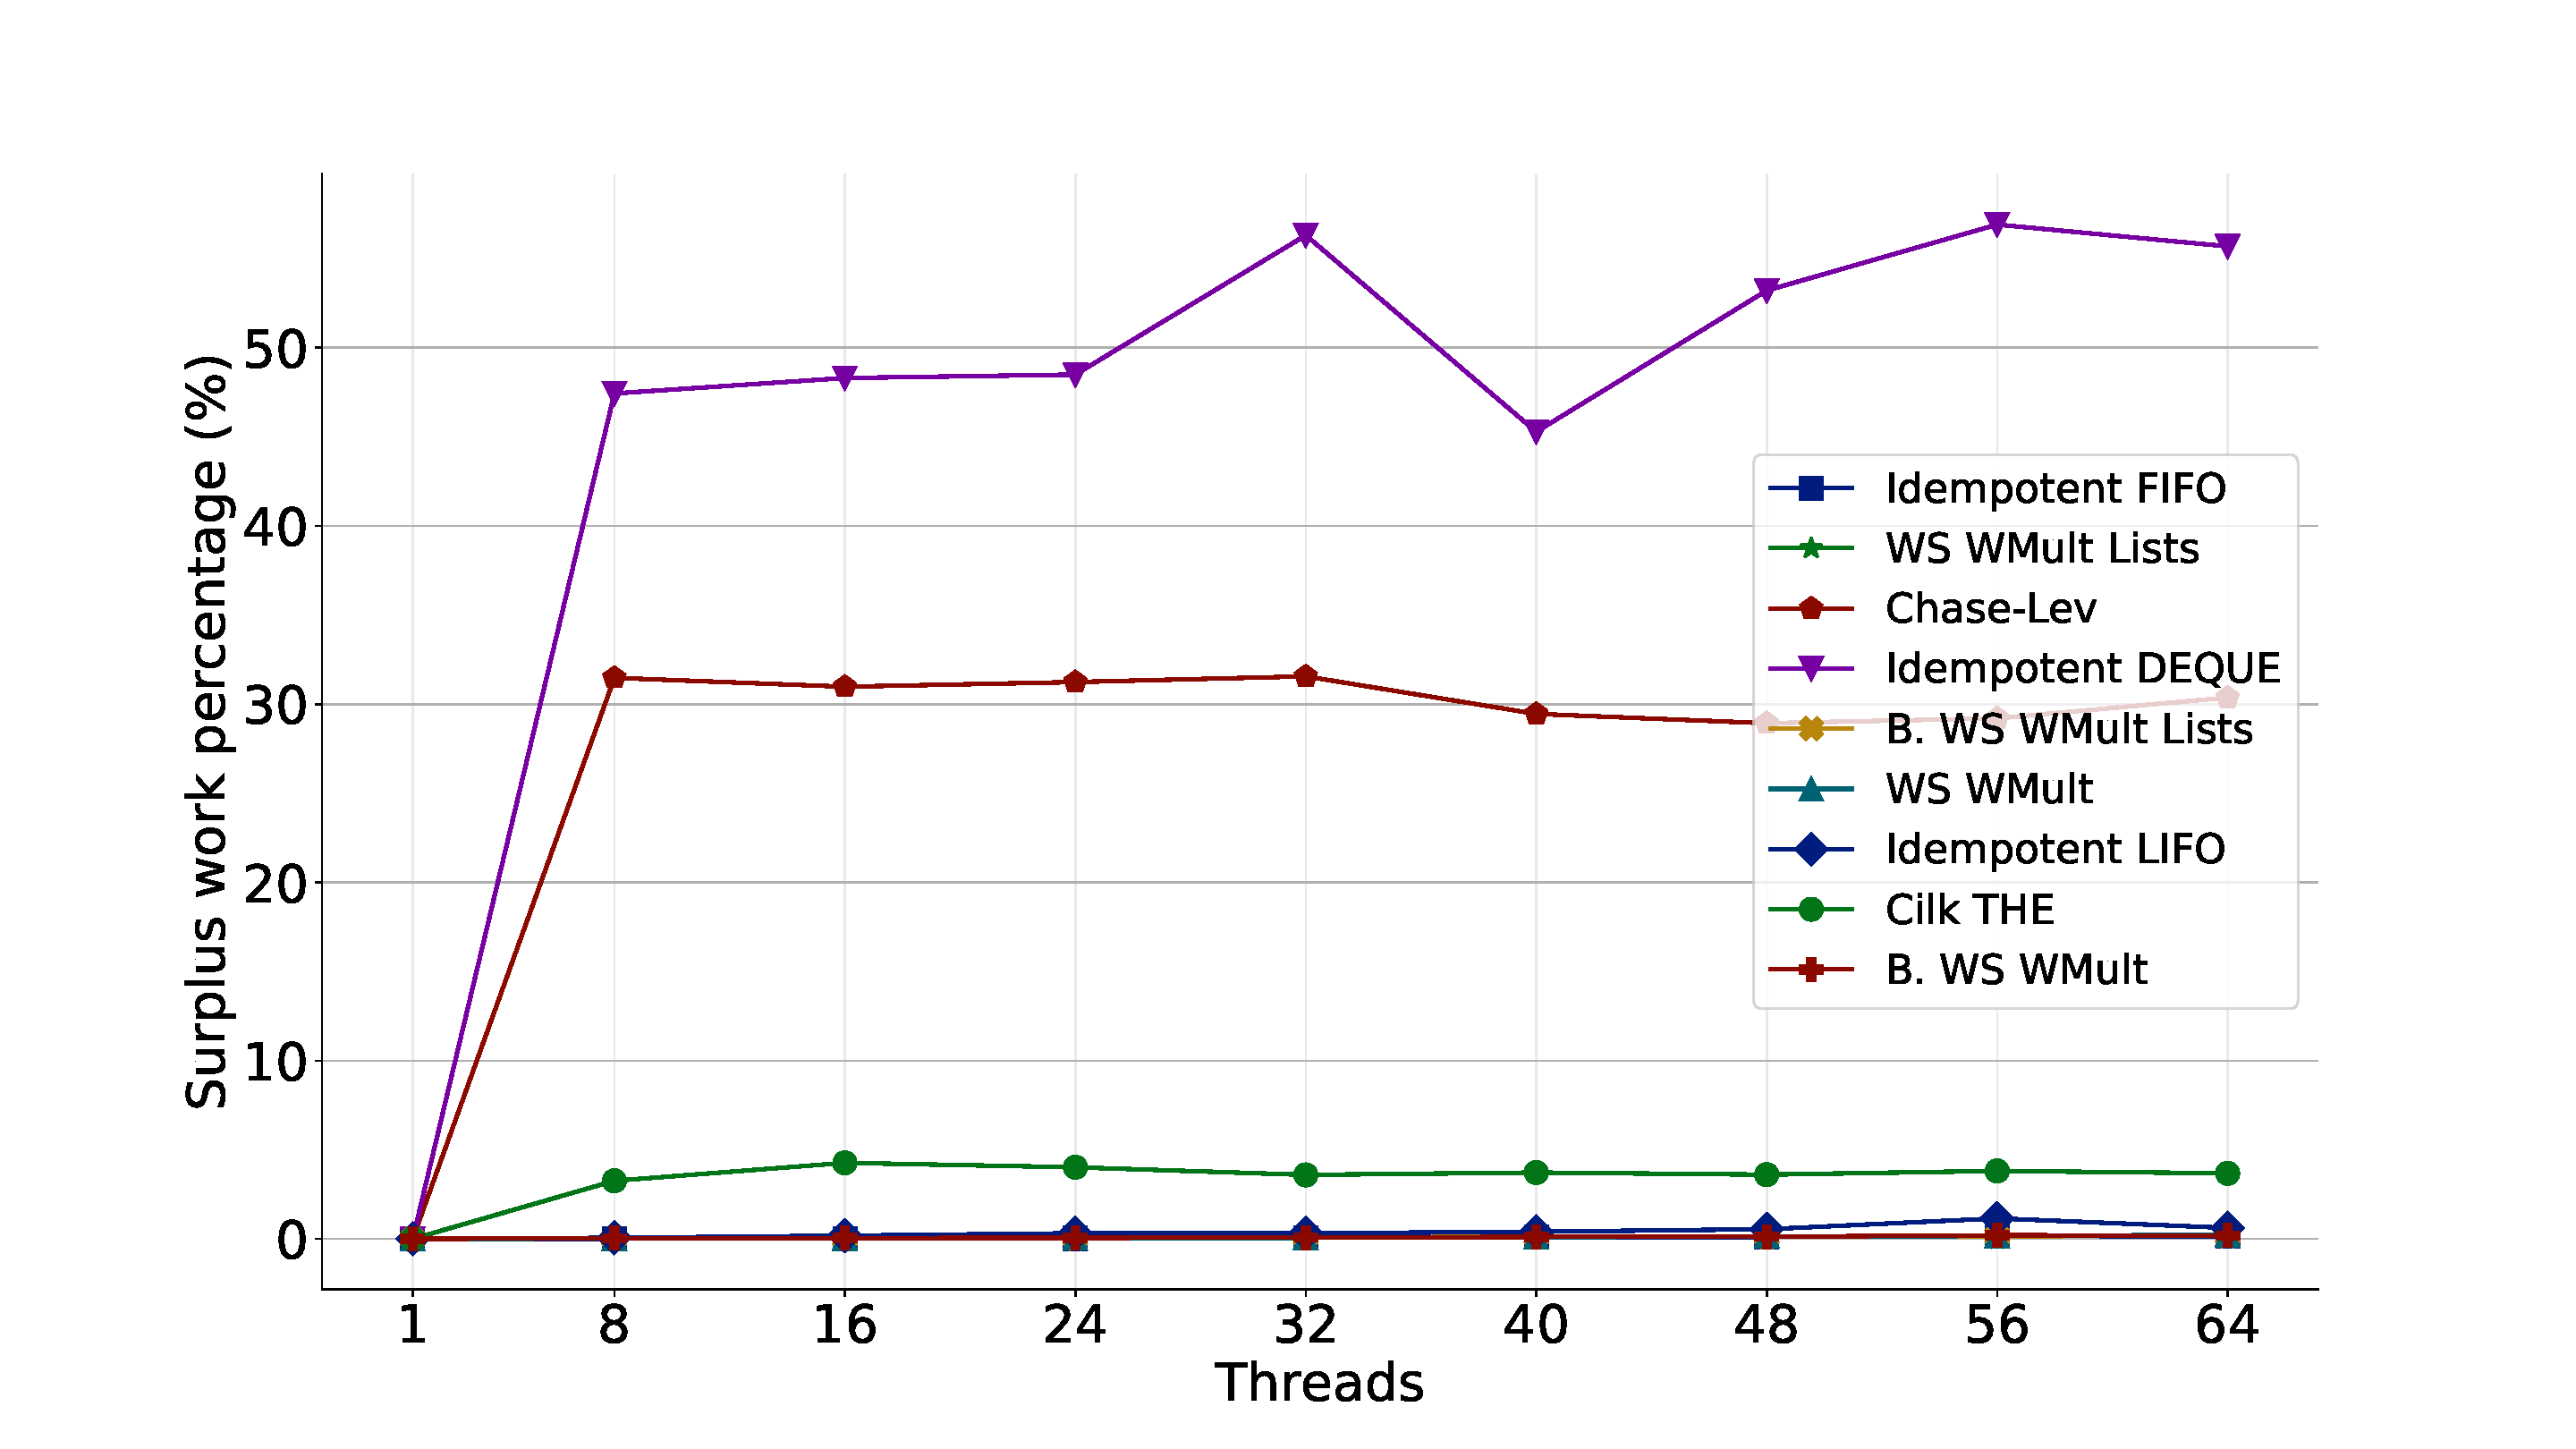
\includegraphics[width=0.48\textwidth]{contents/figures/IV_6_mult-torus_2d_directed_256.pdf}
  }
  \subfloat[\label{fig:surplustorus2ddirected:1000000}Surplus work: Directed Torus 2D. Initial size of 1,000,000 items.]{
    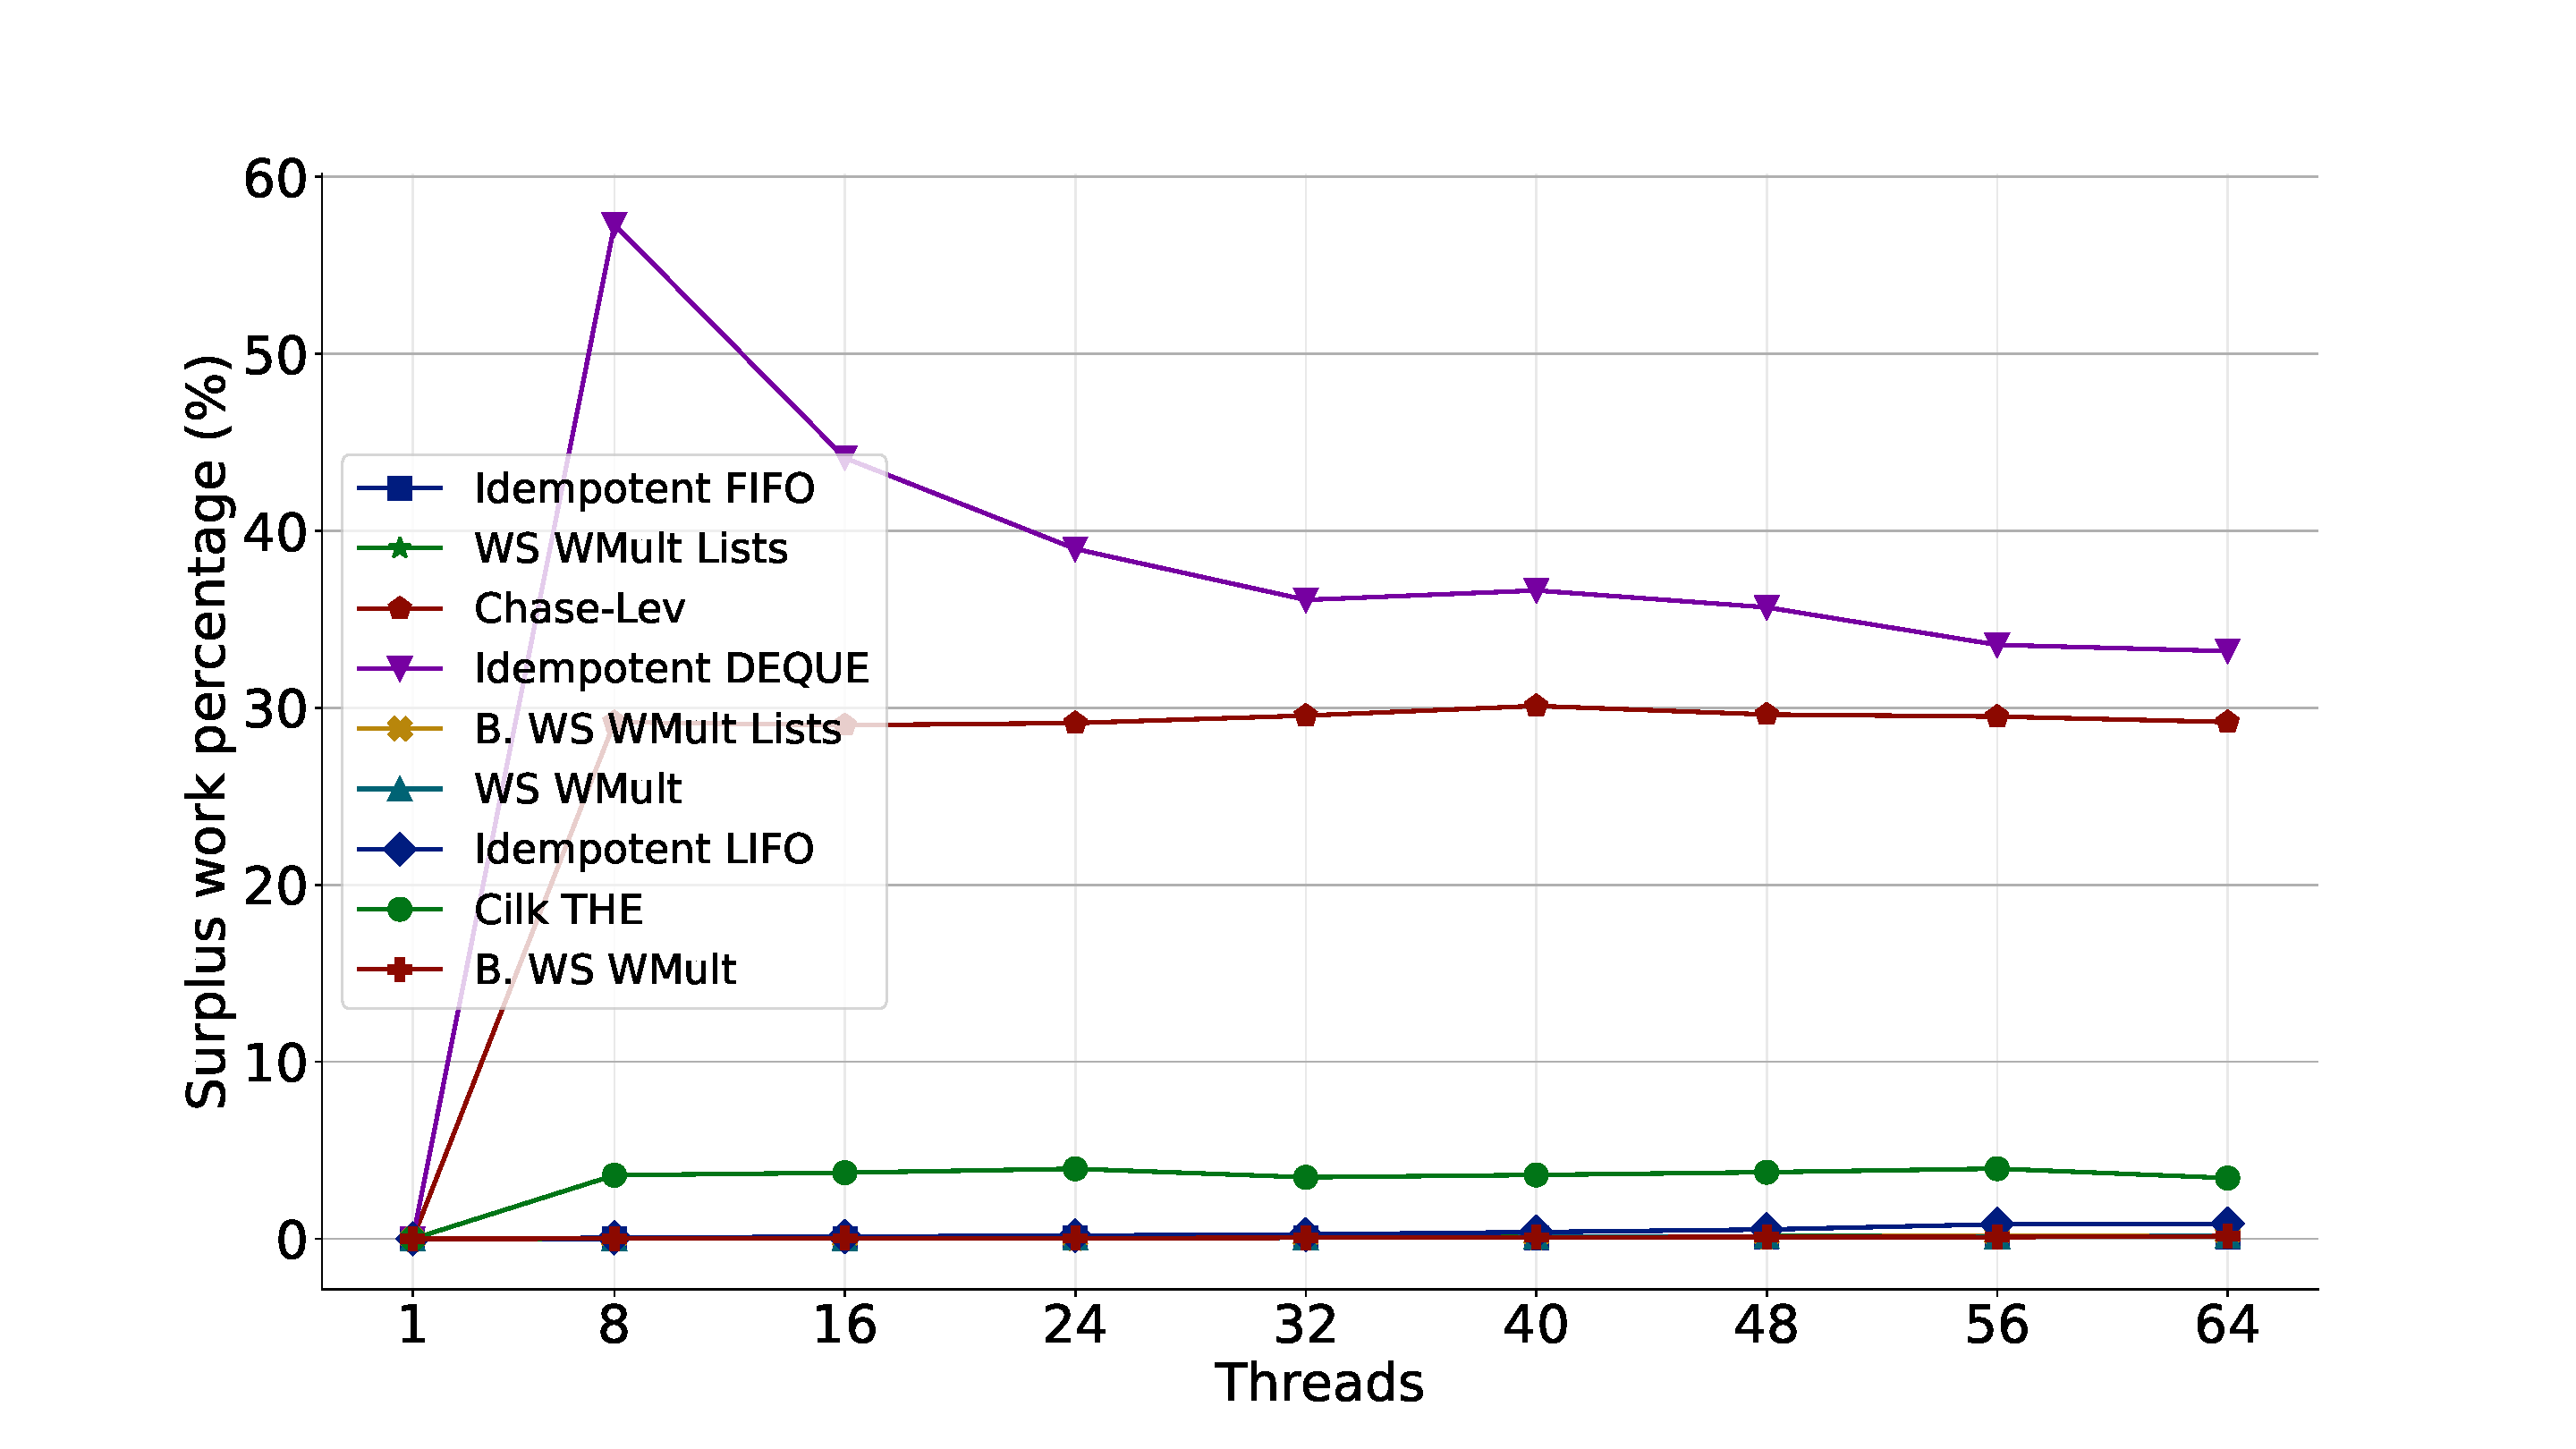
\includegraphics[width=0.48\textwidth]{contents/figures/IV_6_mult-torus_2d_directed_1m.pdf}
  }

  \subfloat[\label{fig:surplustorus3ddirected:256}Surplus work: Directed Torus 3D. Initial size of 256 items.]{
    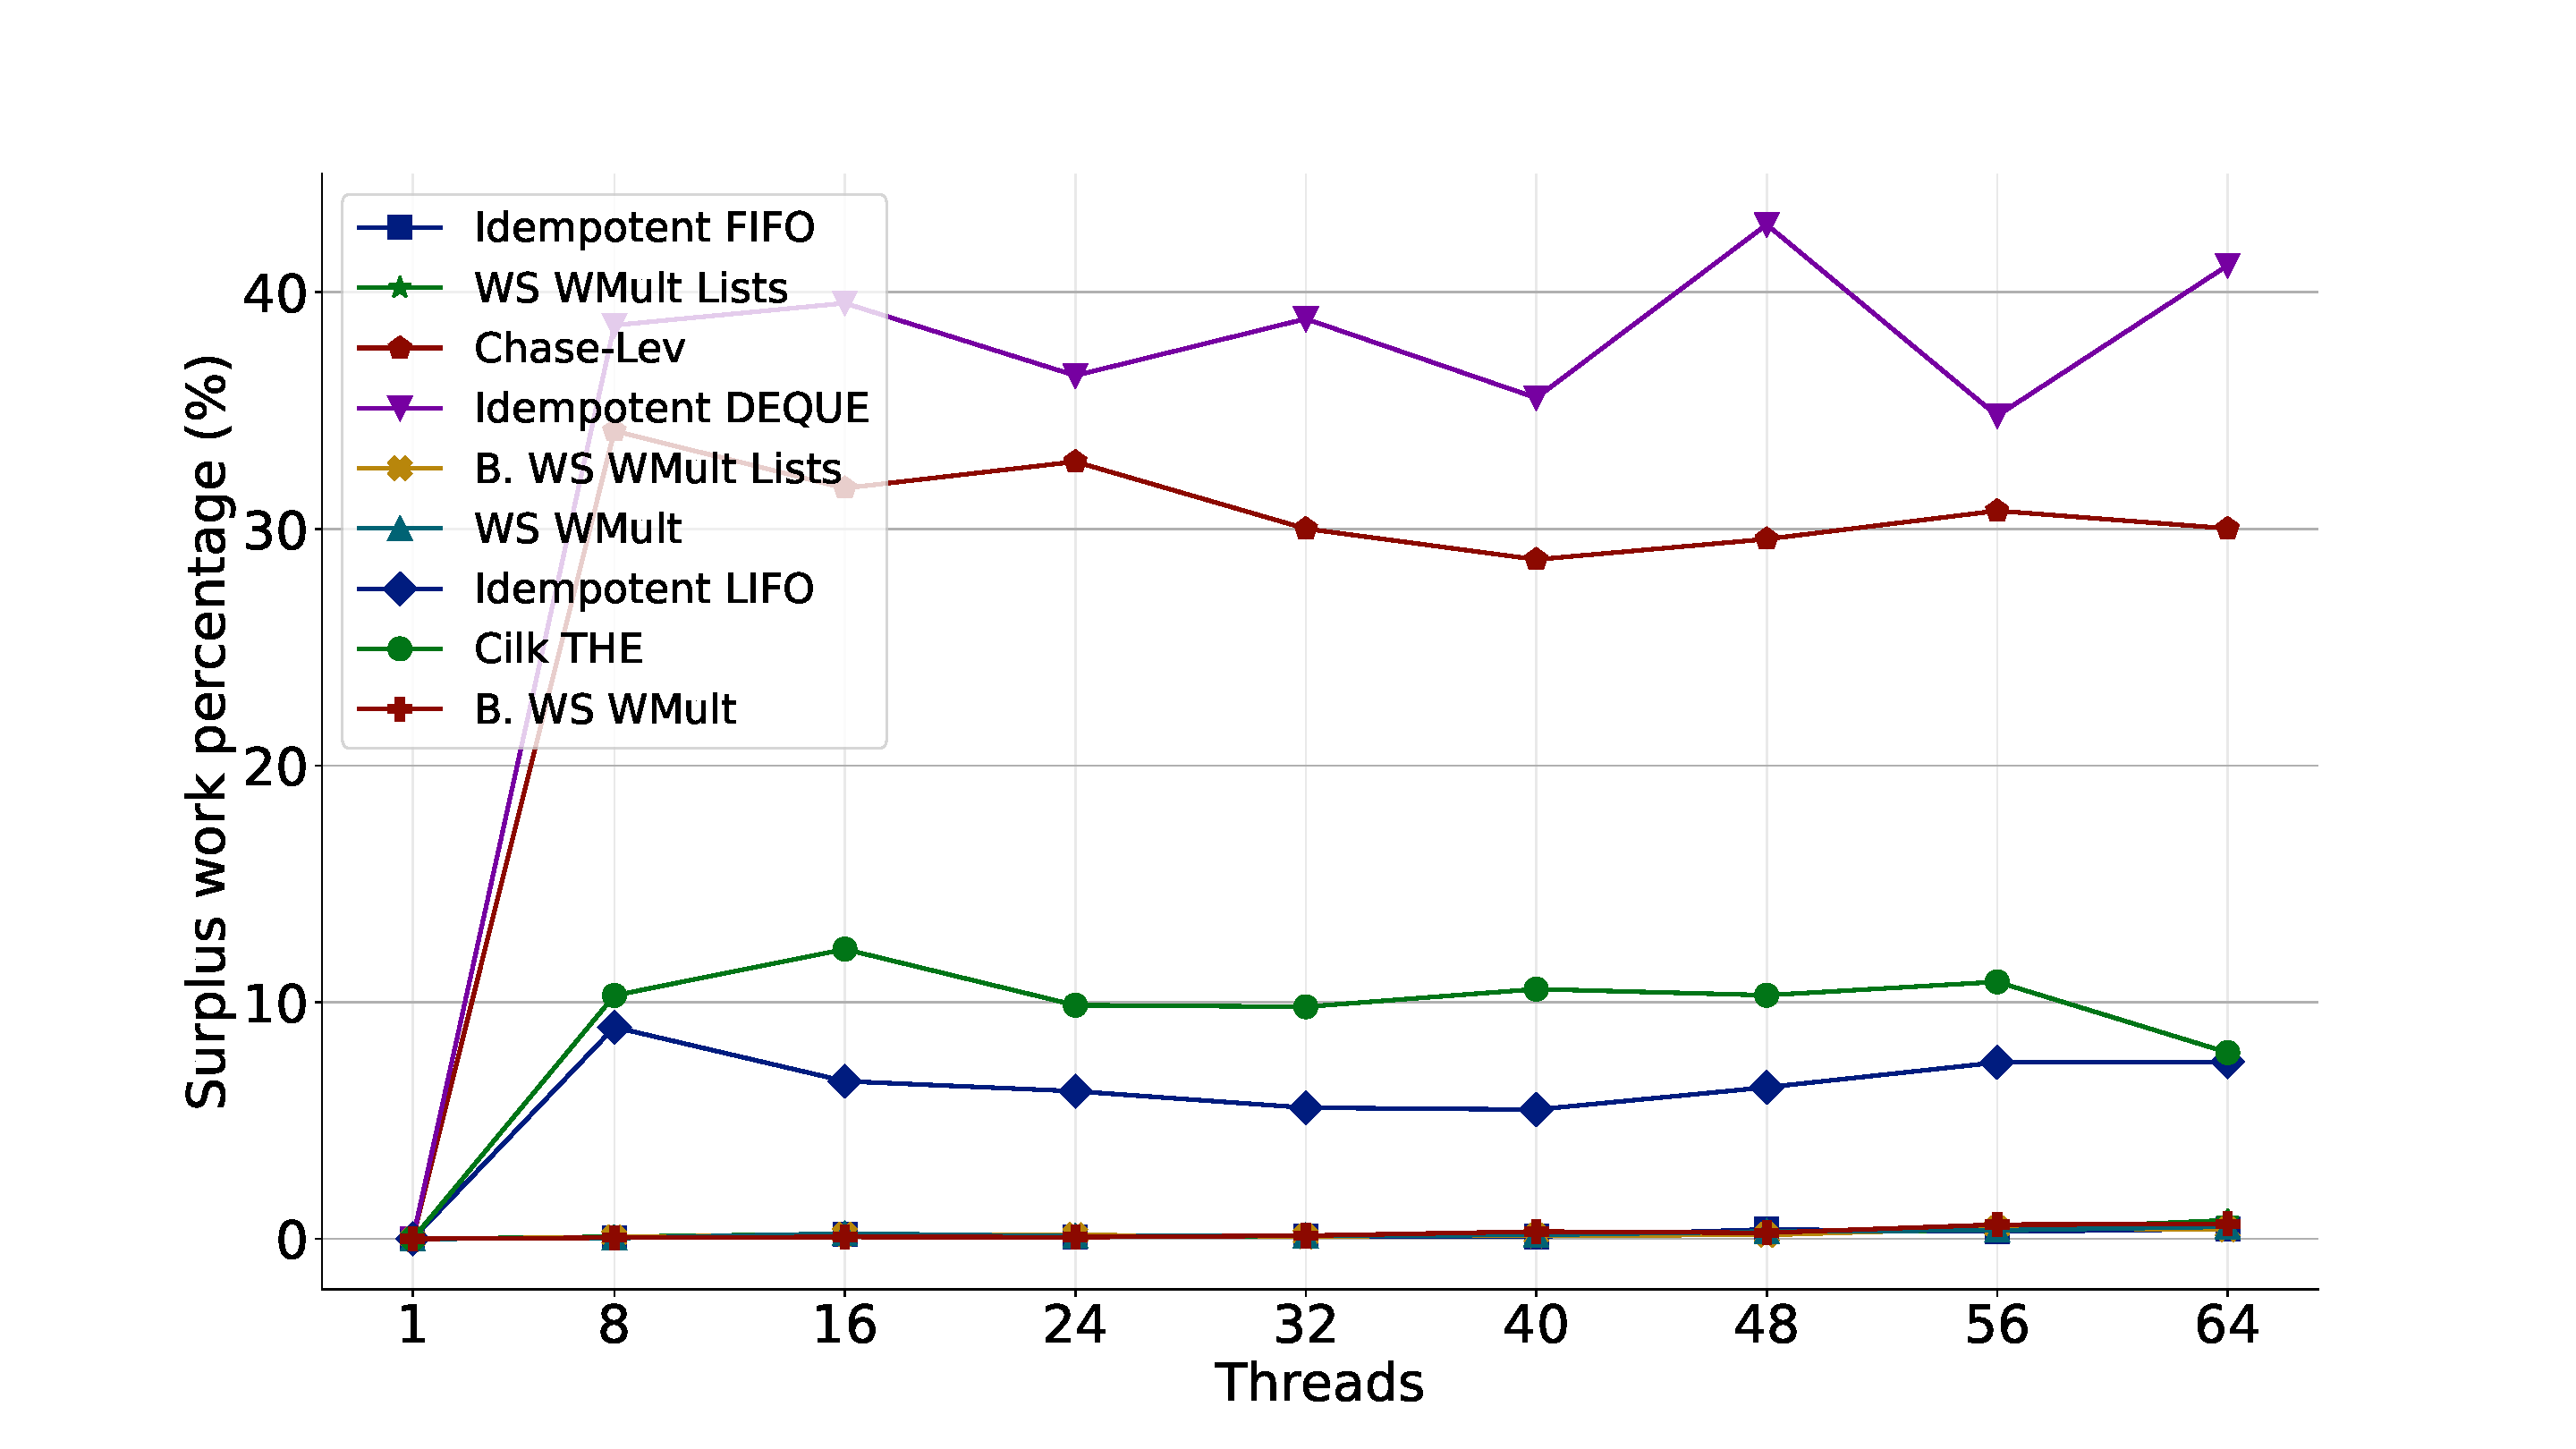
\includegraphics[width=0.48\textwidth]{contents/figures/IV_6_mult-torus_3d_directed_256.pdf}
  }
  \subfloat[\label{fig:surplustorus3ddirected:1000000}Surplus work: Directed Torus 3D. Initial size of 1,000,000 items.]{
    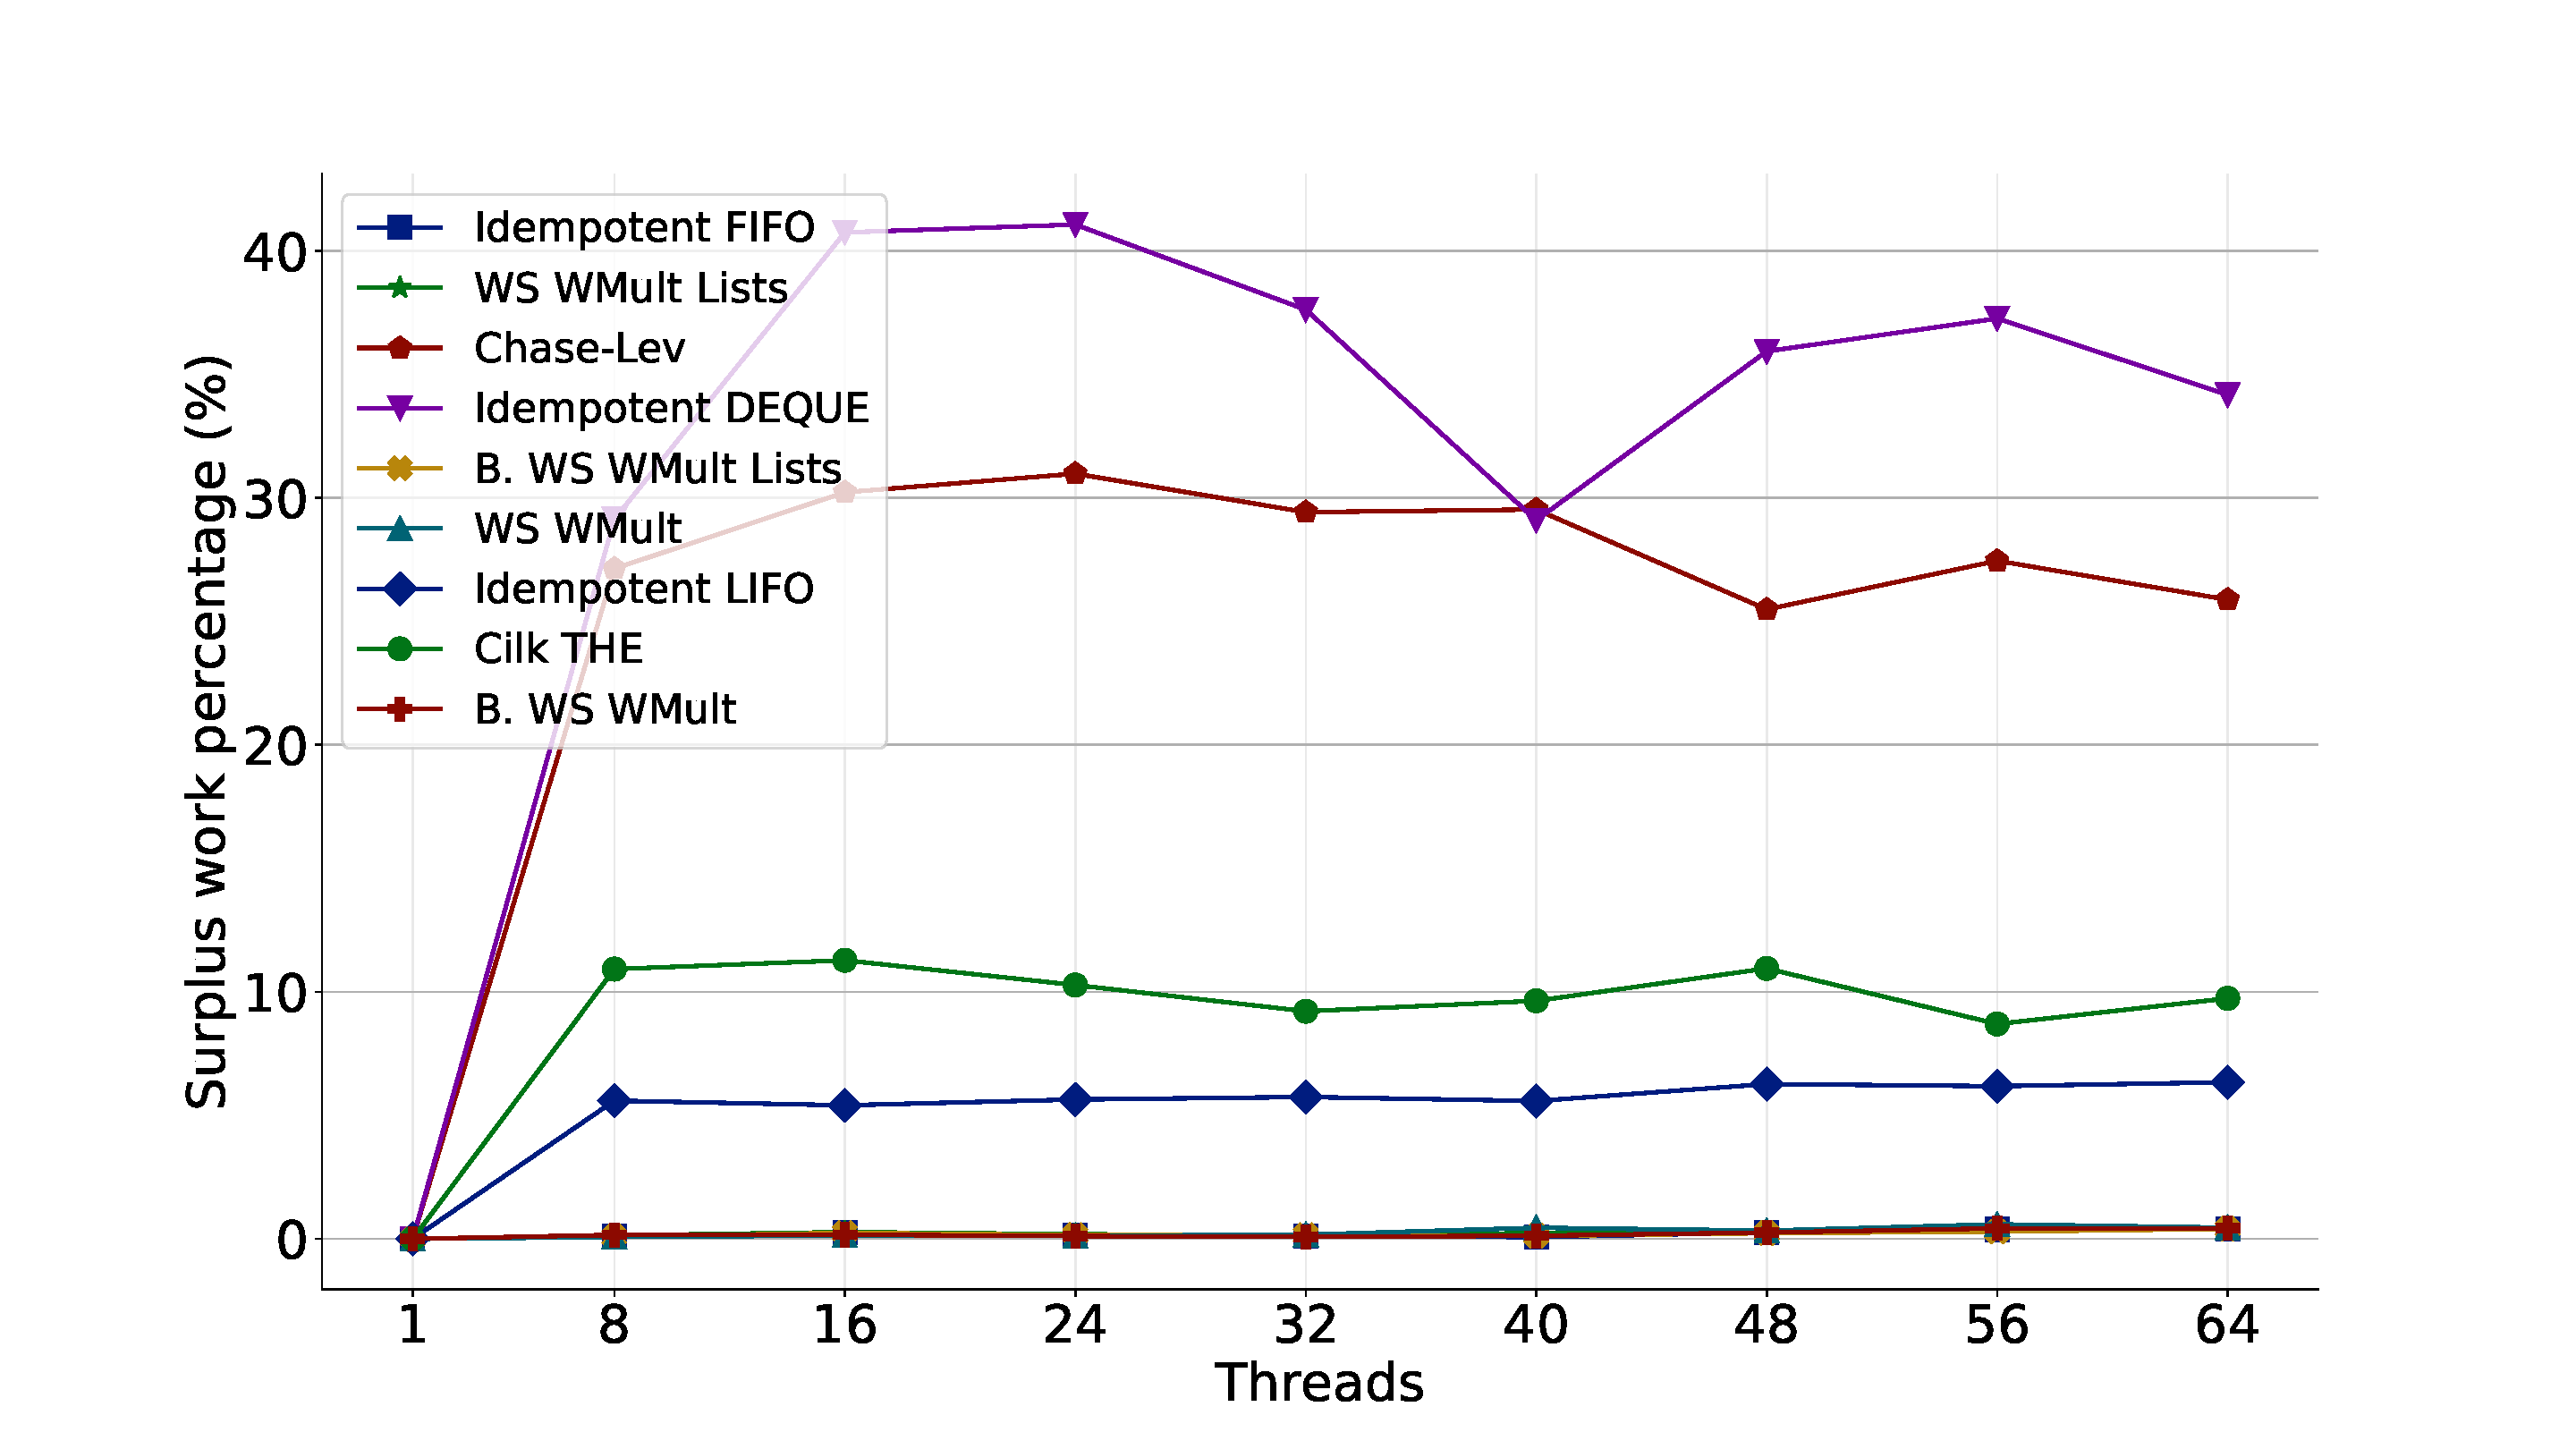
\includegraphics[width=0.48\textwidth]{contents/figures/IV_6_mult-torus_3d_directed_1m.pdf}
  }

  \subfloat[\label{fig:surplusrandom:256}Surplus work: Directed Random. Initial size of 256 items.]{
    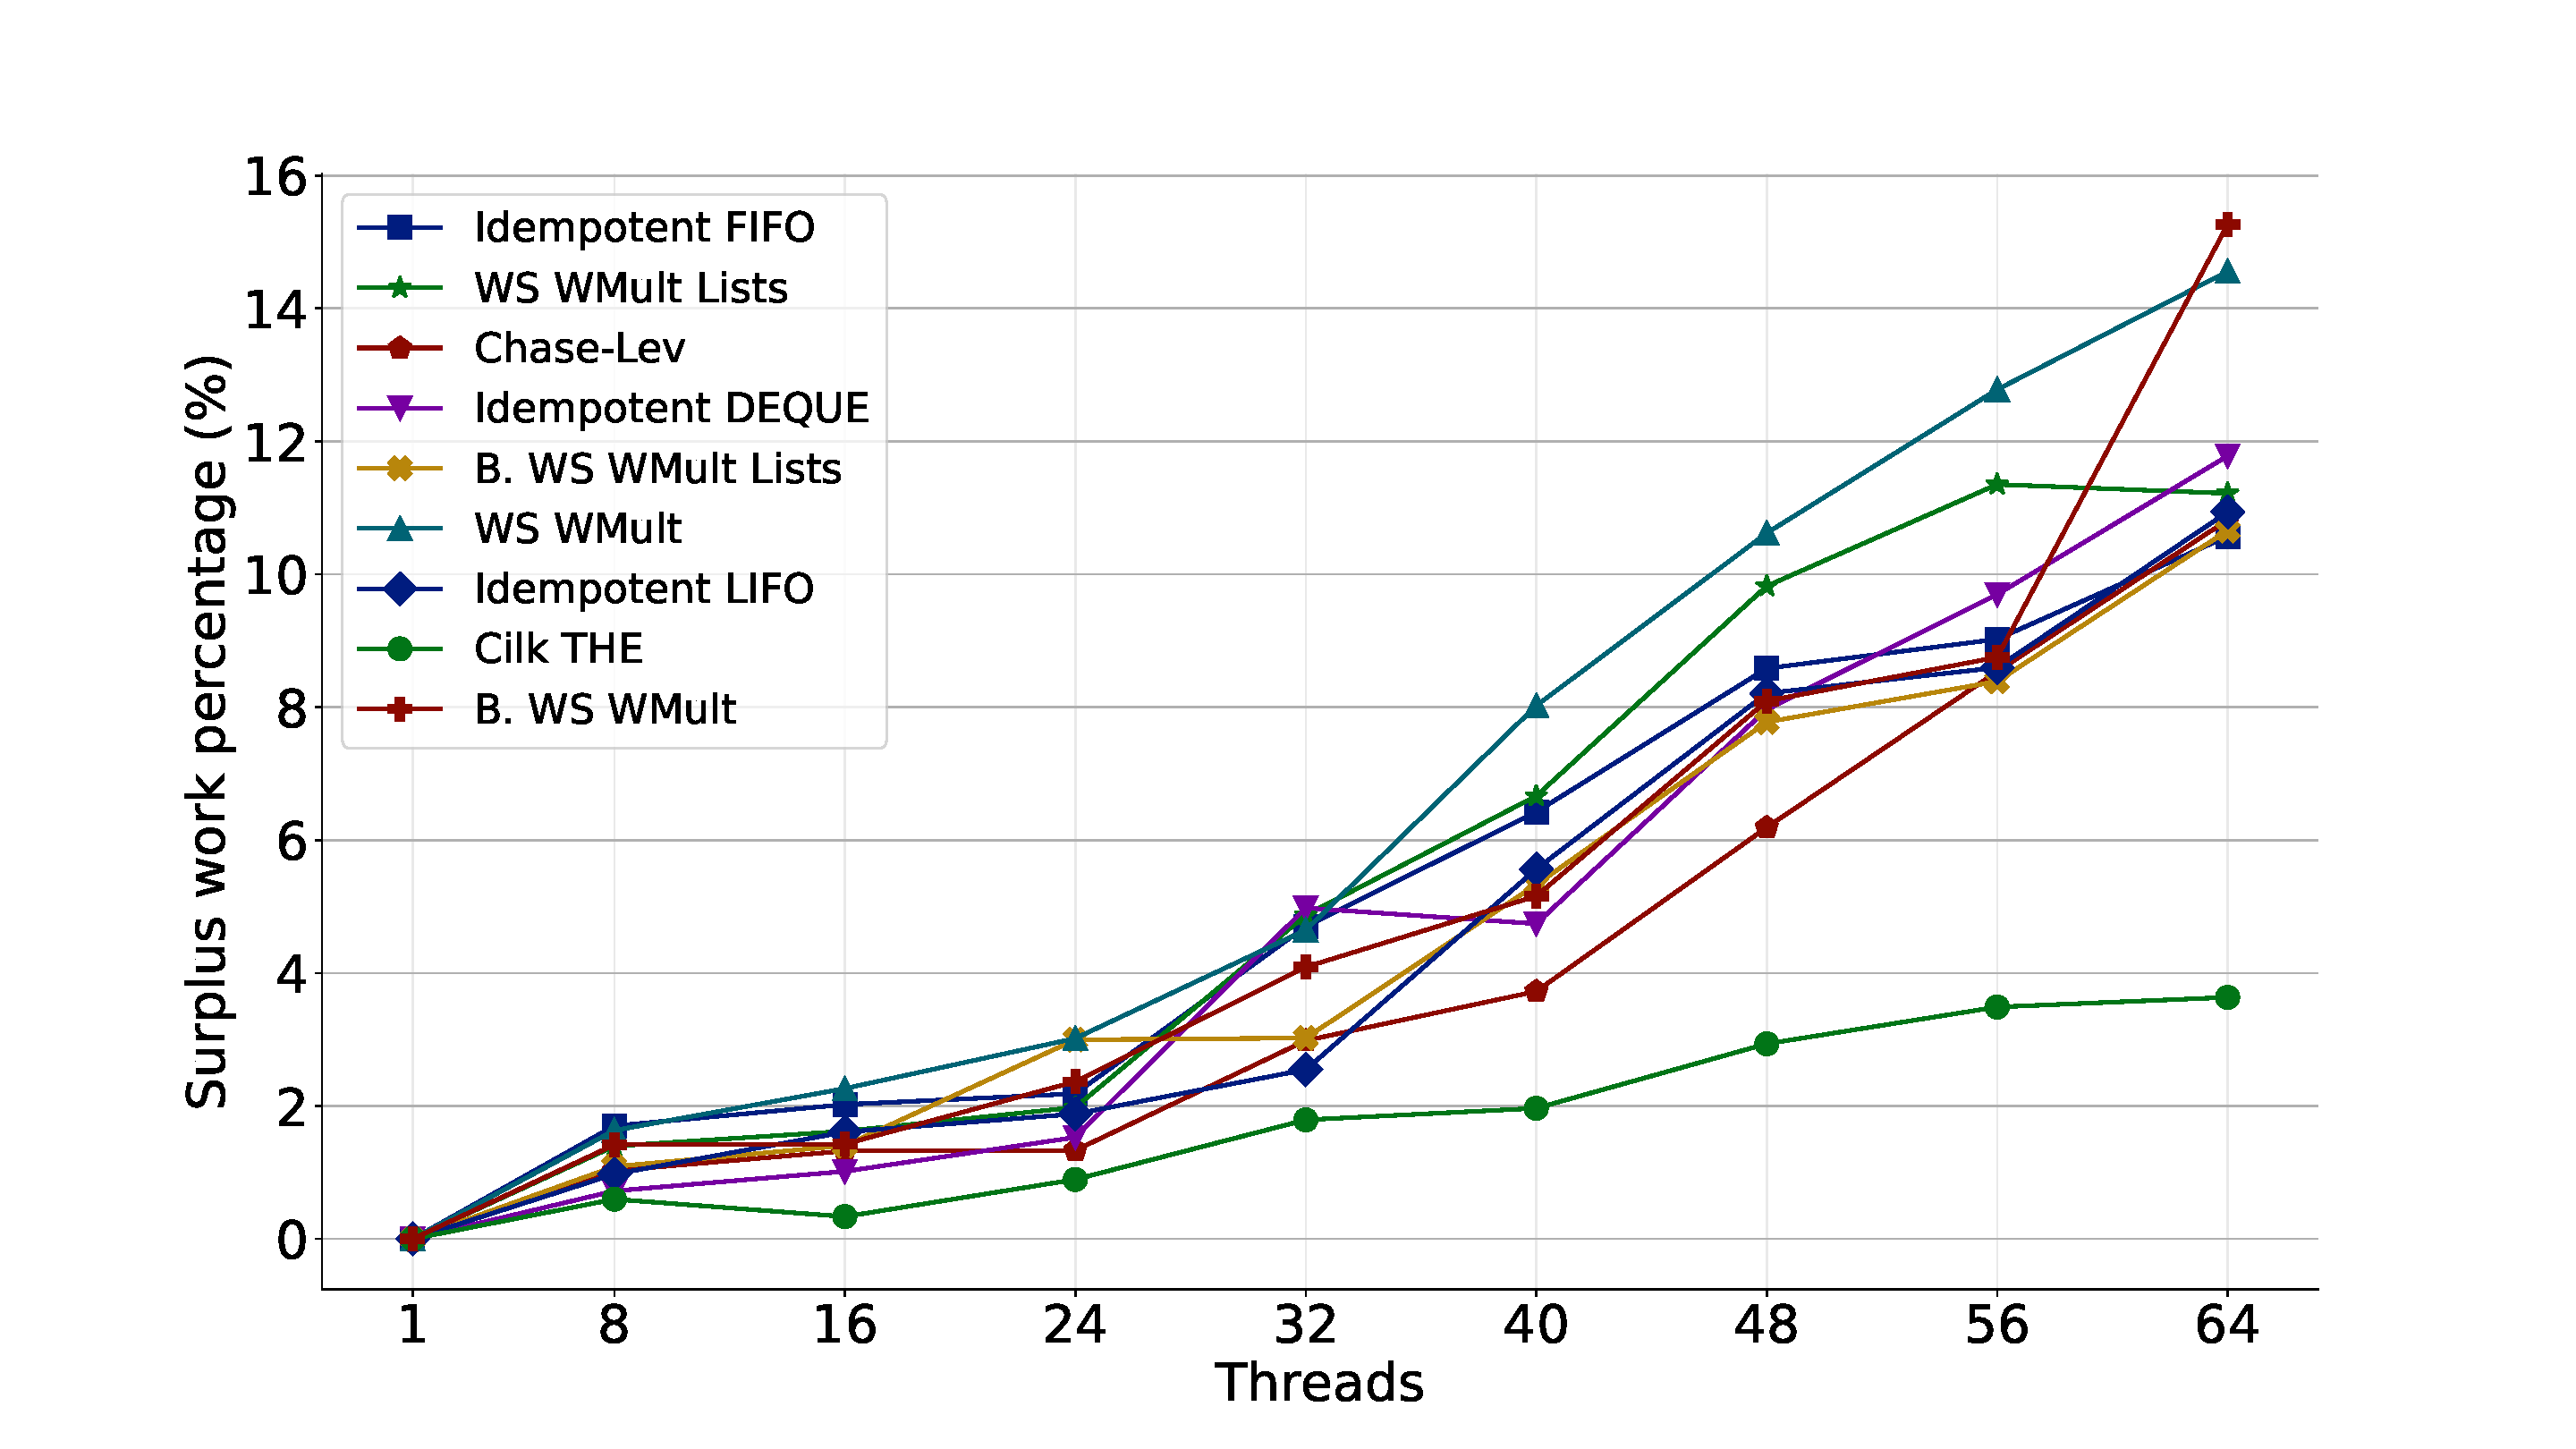
\includegraphics[width=0.48\textwidth]{contents/figures/IV_6_mult-random_directed_256.pdf}
  }
  \subfloat[\label{fig:surplusrandom:1000000}Surplus work: Directed Random: Initial size of 1,000,000 items.]{
    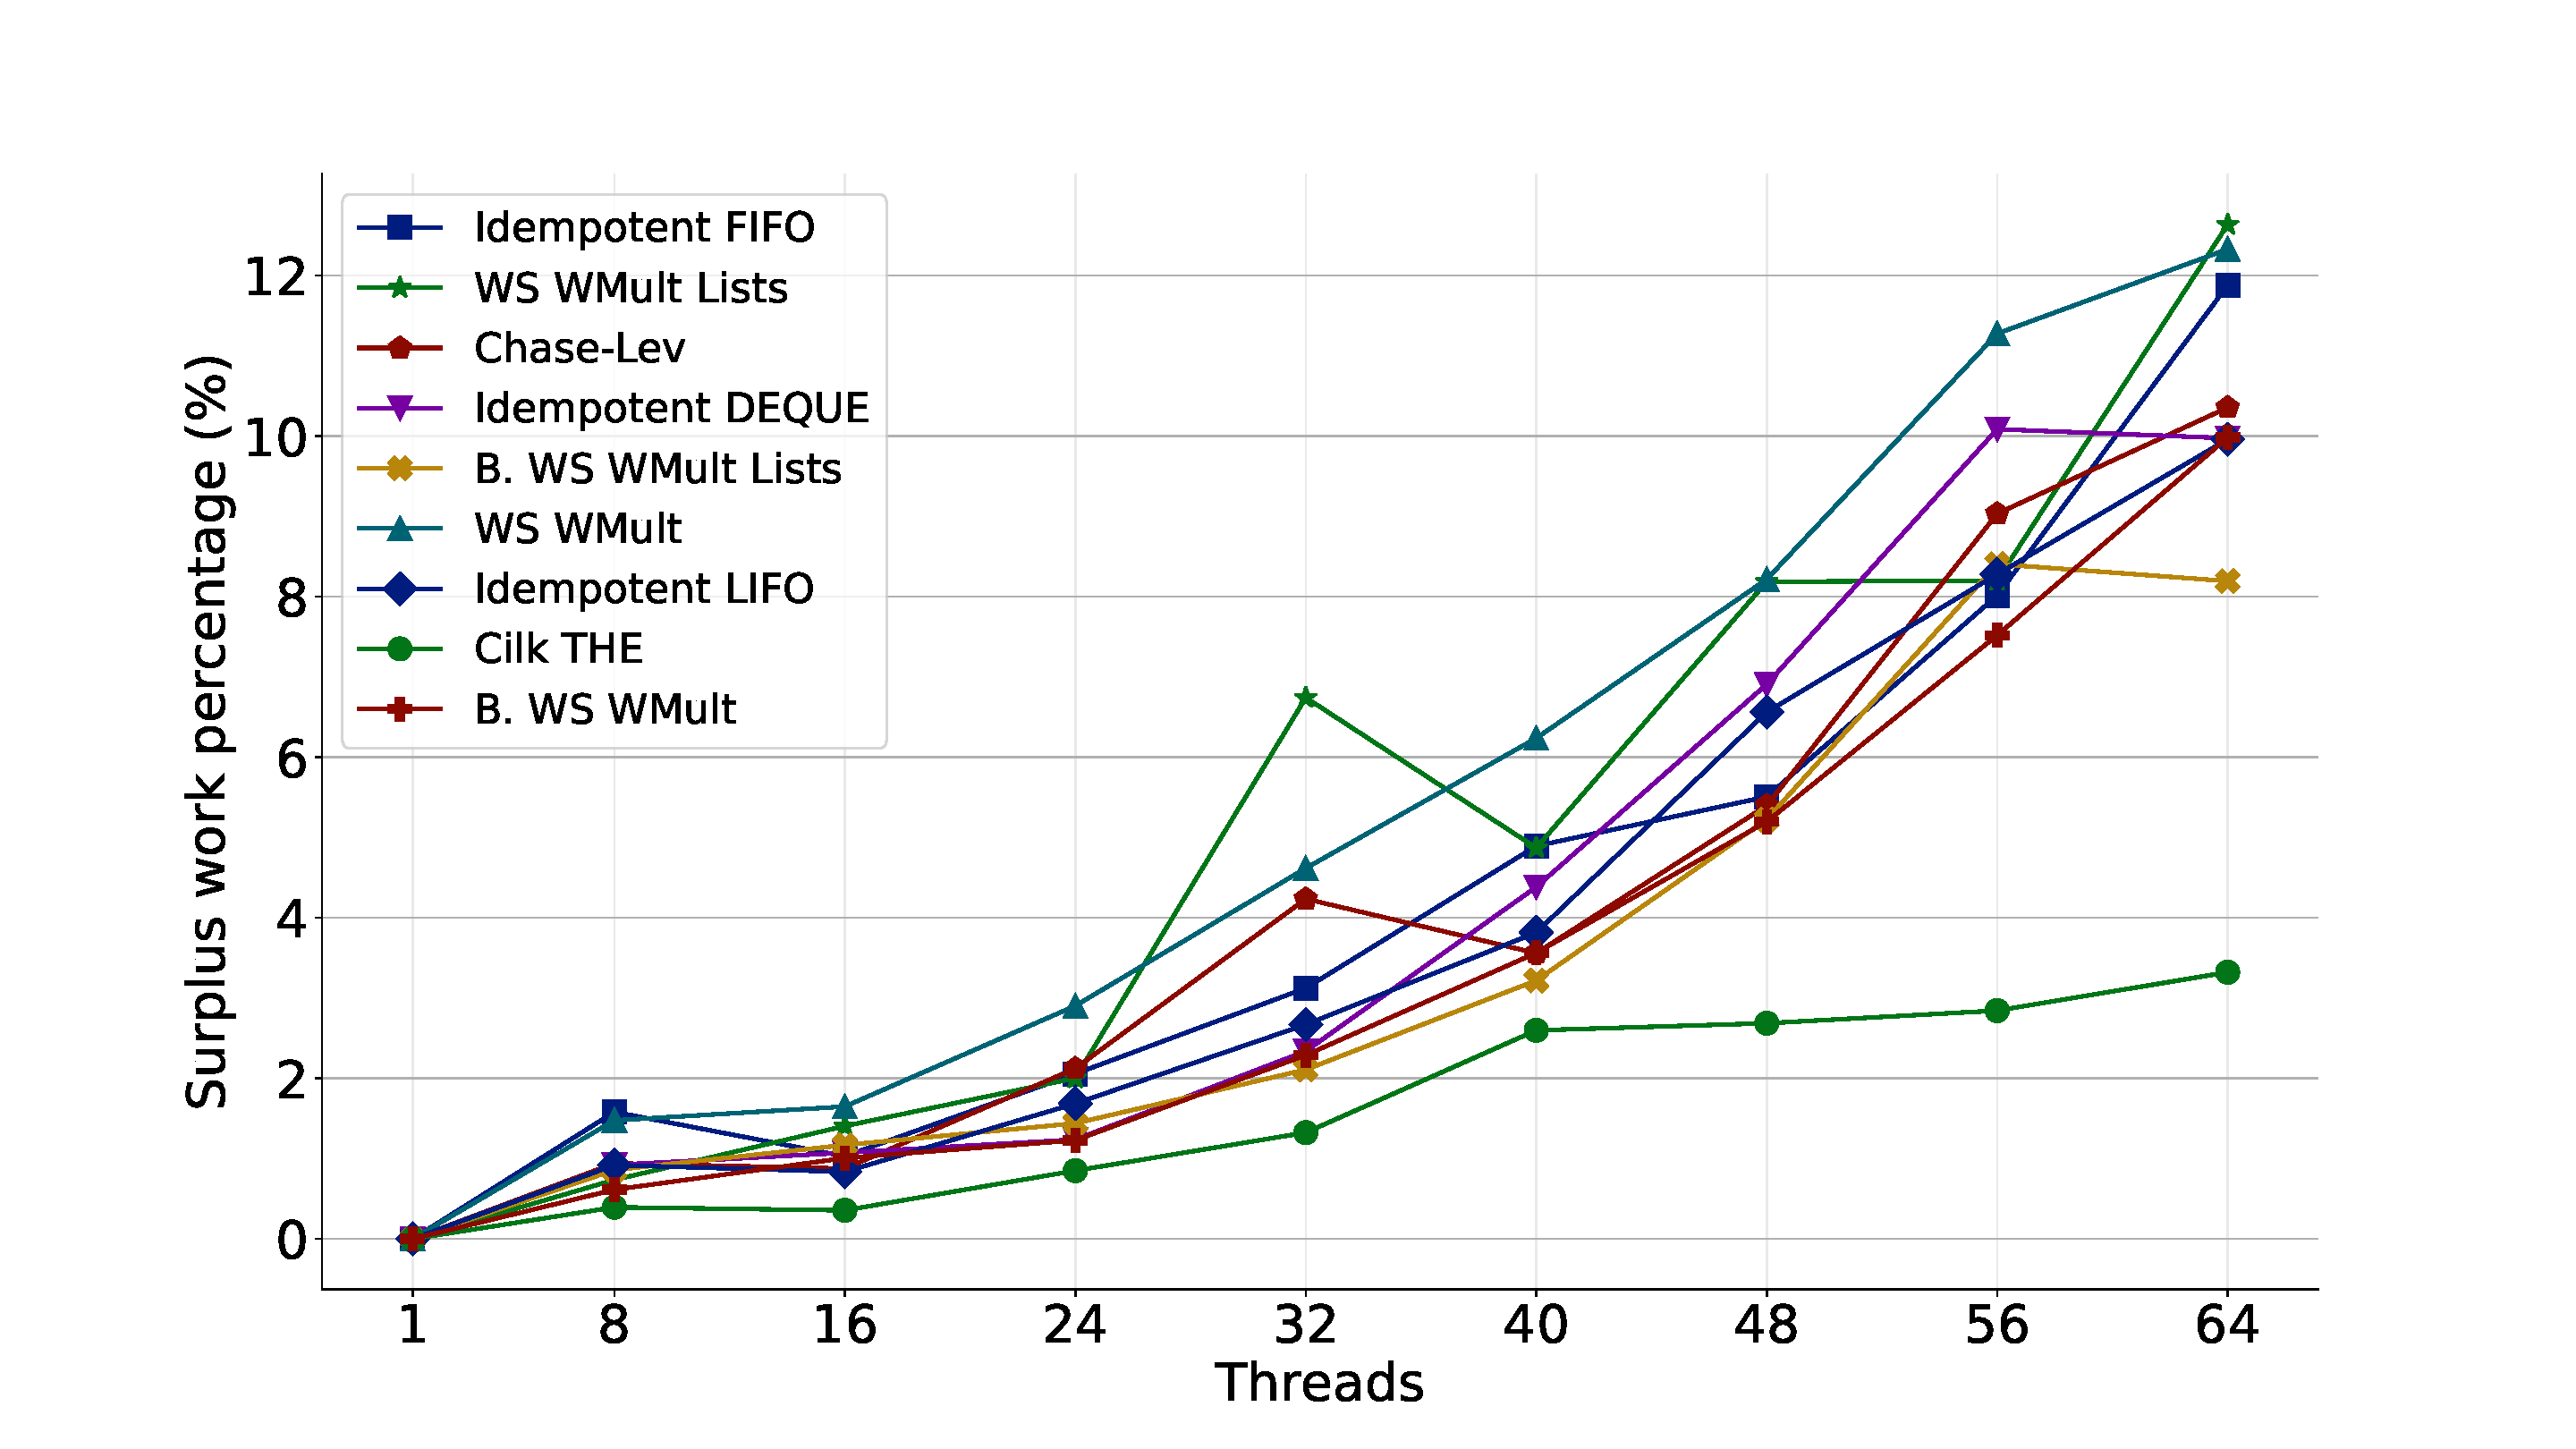
\includegraphics[width=0.48\textwidth]{contents/figures/IV_6_mult-random_directed_1m.pdf}
  }

  \caption{\label{fig:surplusgraphapplication} Surplus work (percentage) of the experiments.  Surplus work: the difference between the total number of \Puts and the number of puts in sequential executions (i.e., $1,000,000$).}
\end{figure}

\begin{figure}[!ht]
  \subfloat[\label{fig:exec-surplustorus2ddirected:256}Executed surplus work: Directed Torus 2D. Initial size of 256 items.]{
    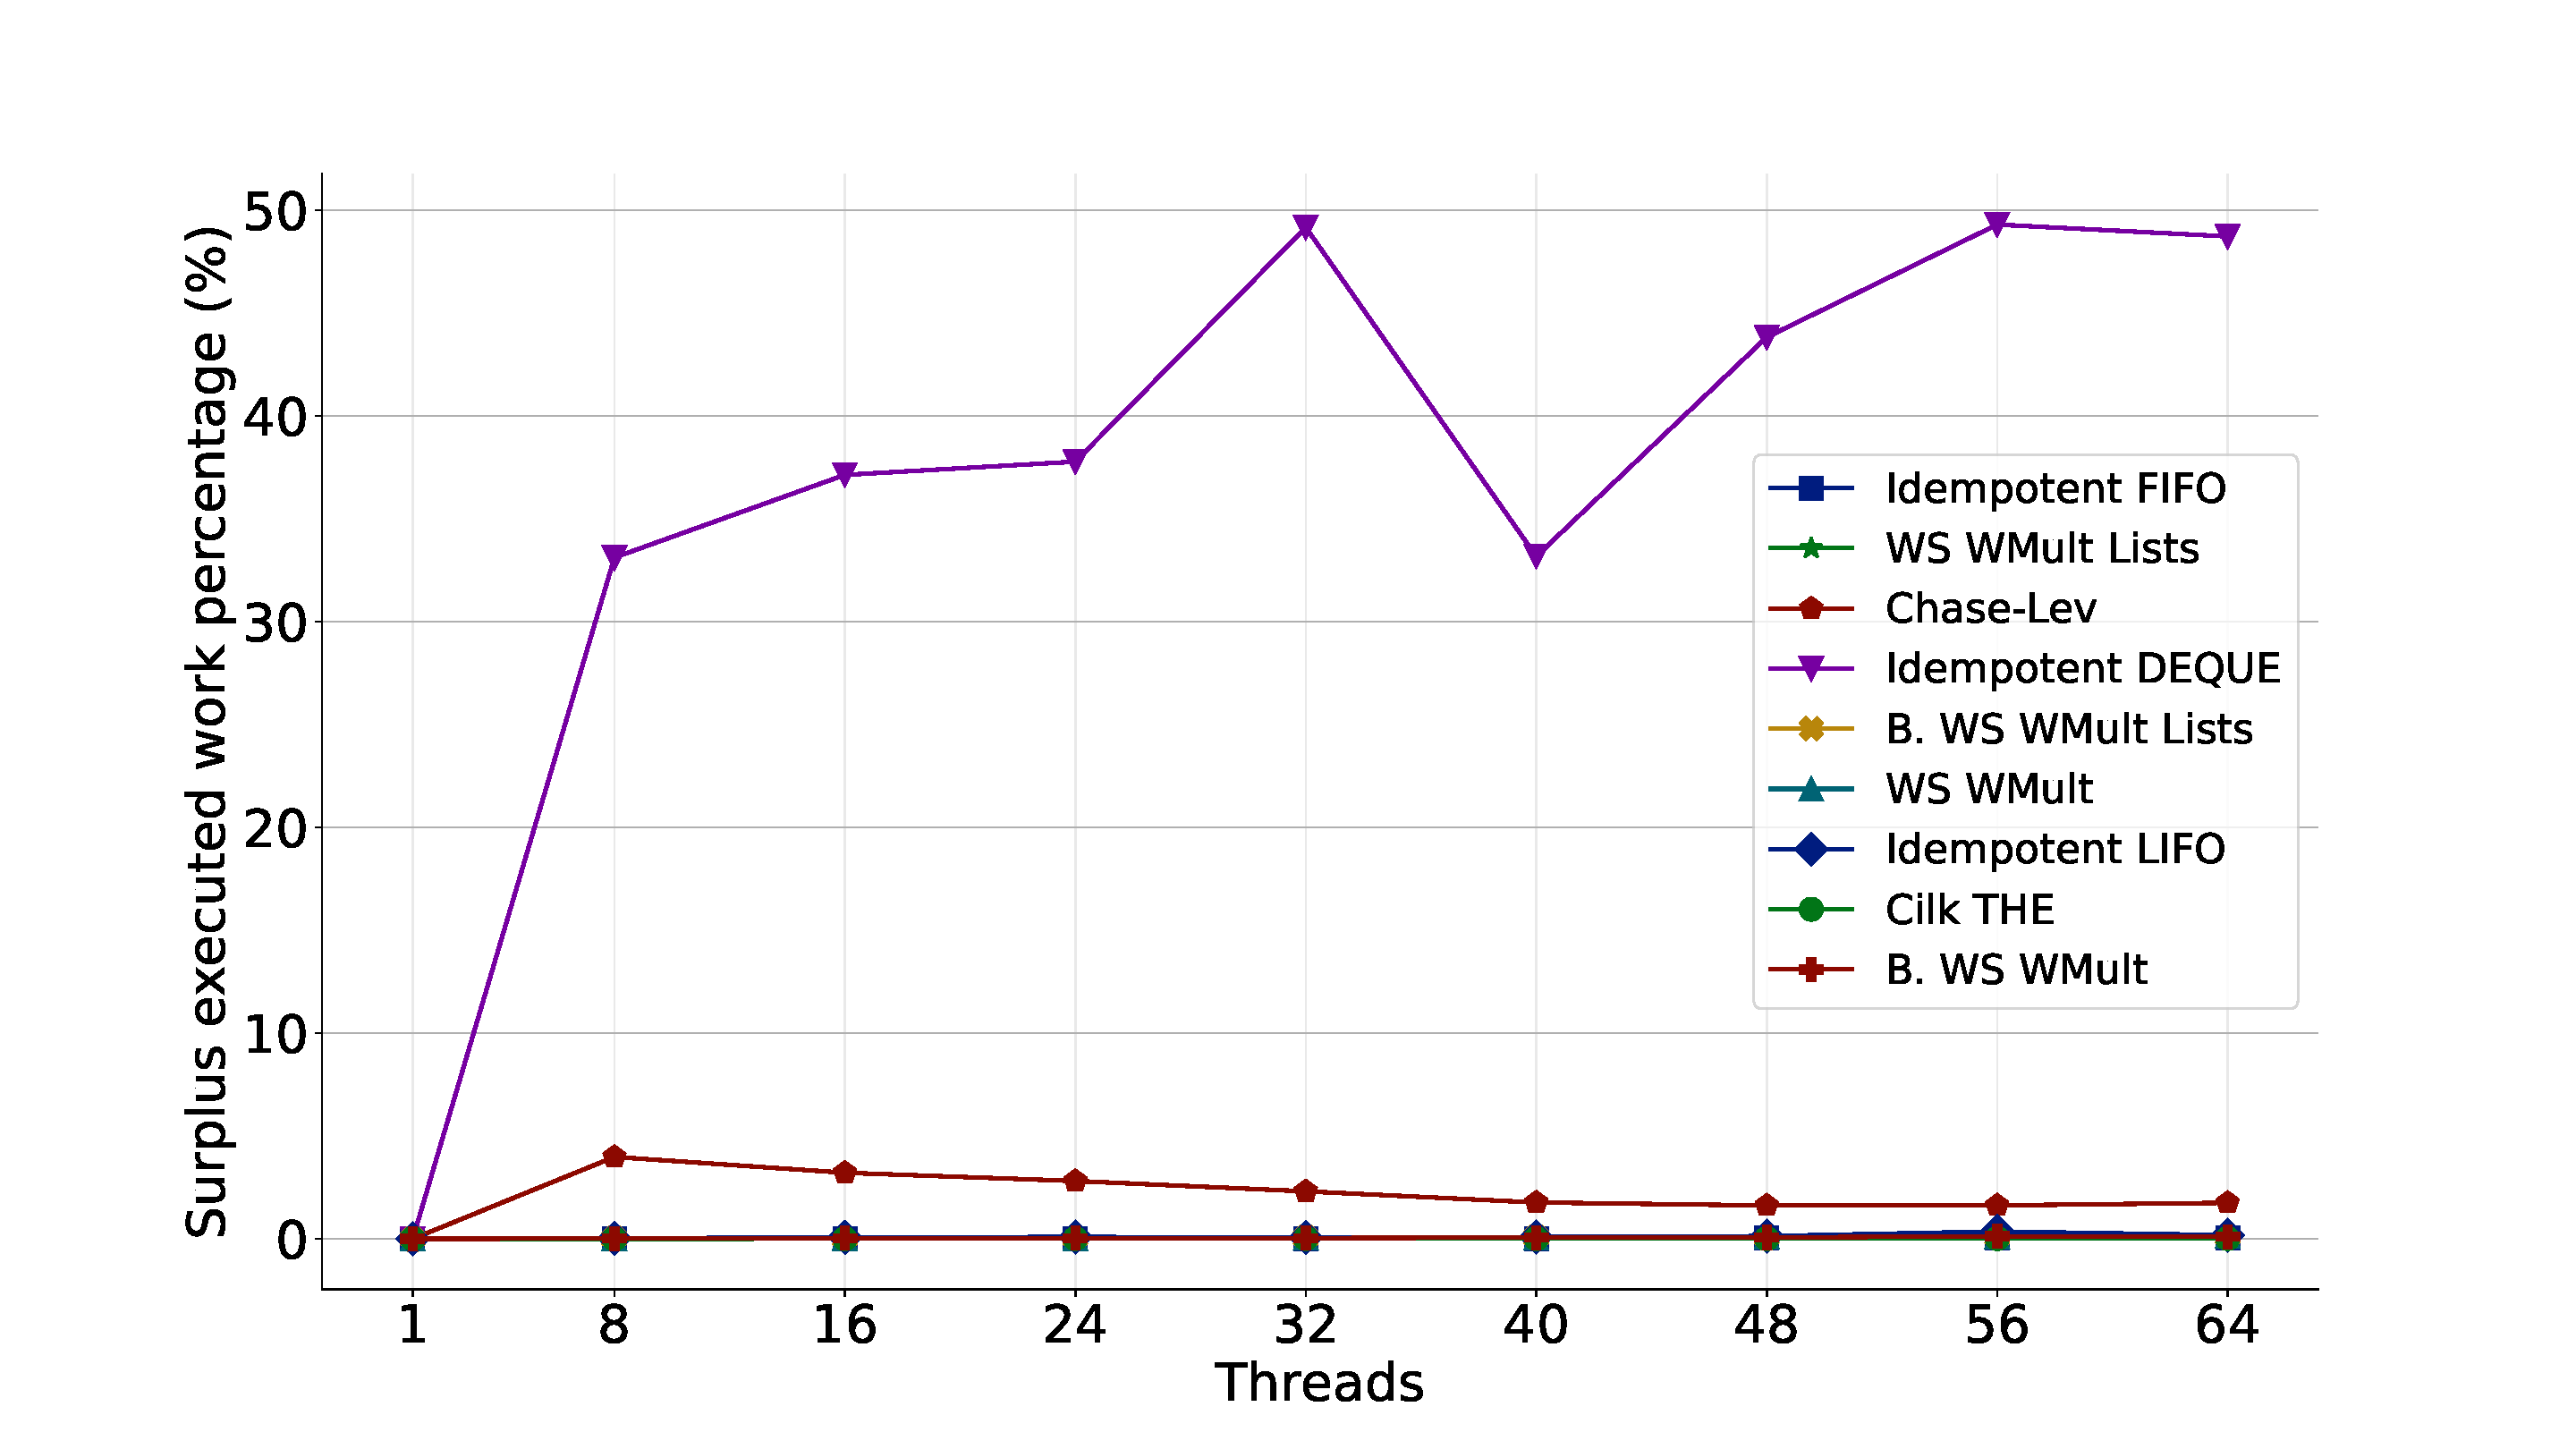
\includegraphics[width=0.48\textwidth]{contents/figures/IV_6_mult-exec-torus_2d_directed_256.pdf}
  }
  \subfloat[\label{fig:exec-surplustorus2ddirected:1000000}Executed surplus work: Directed Torus 2D. Initial size of 1,000,000 items.]{
    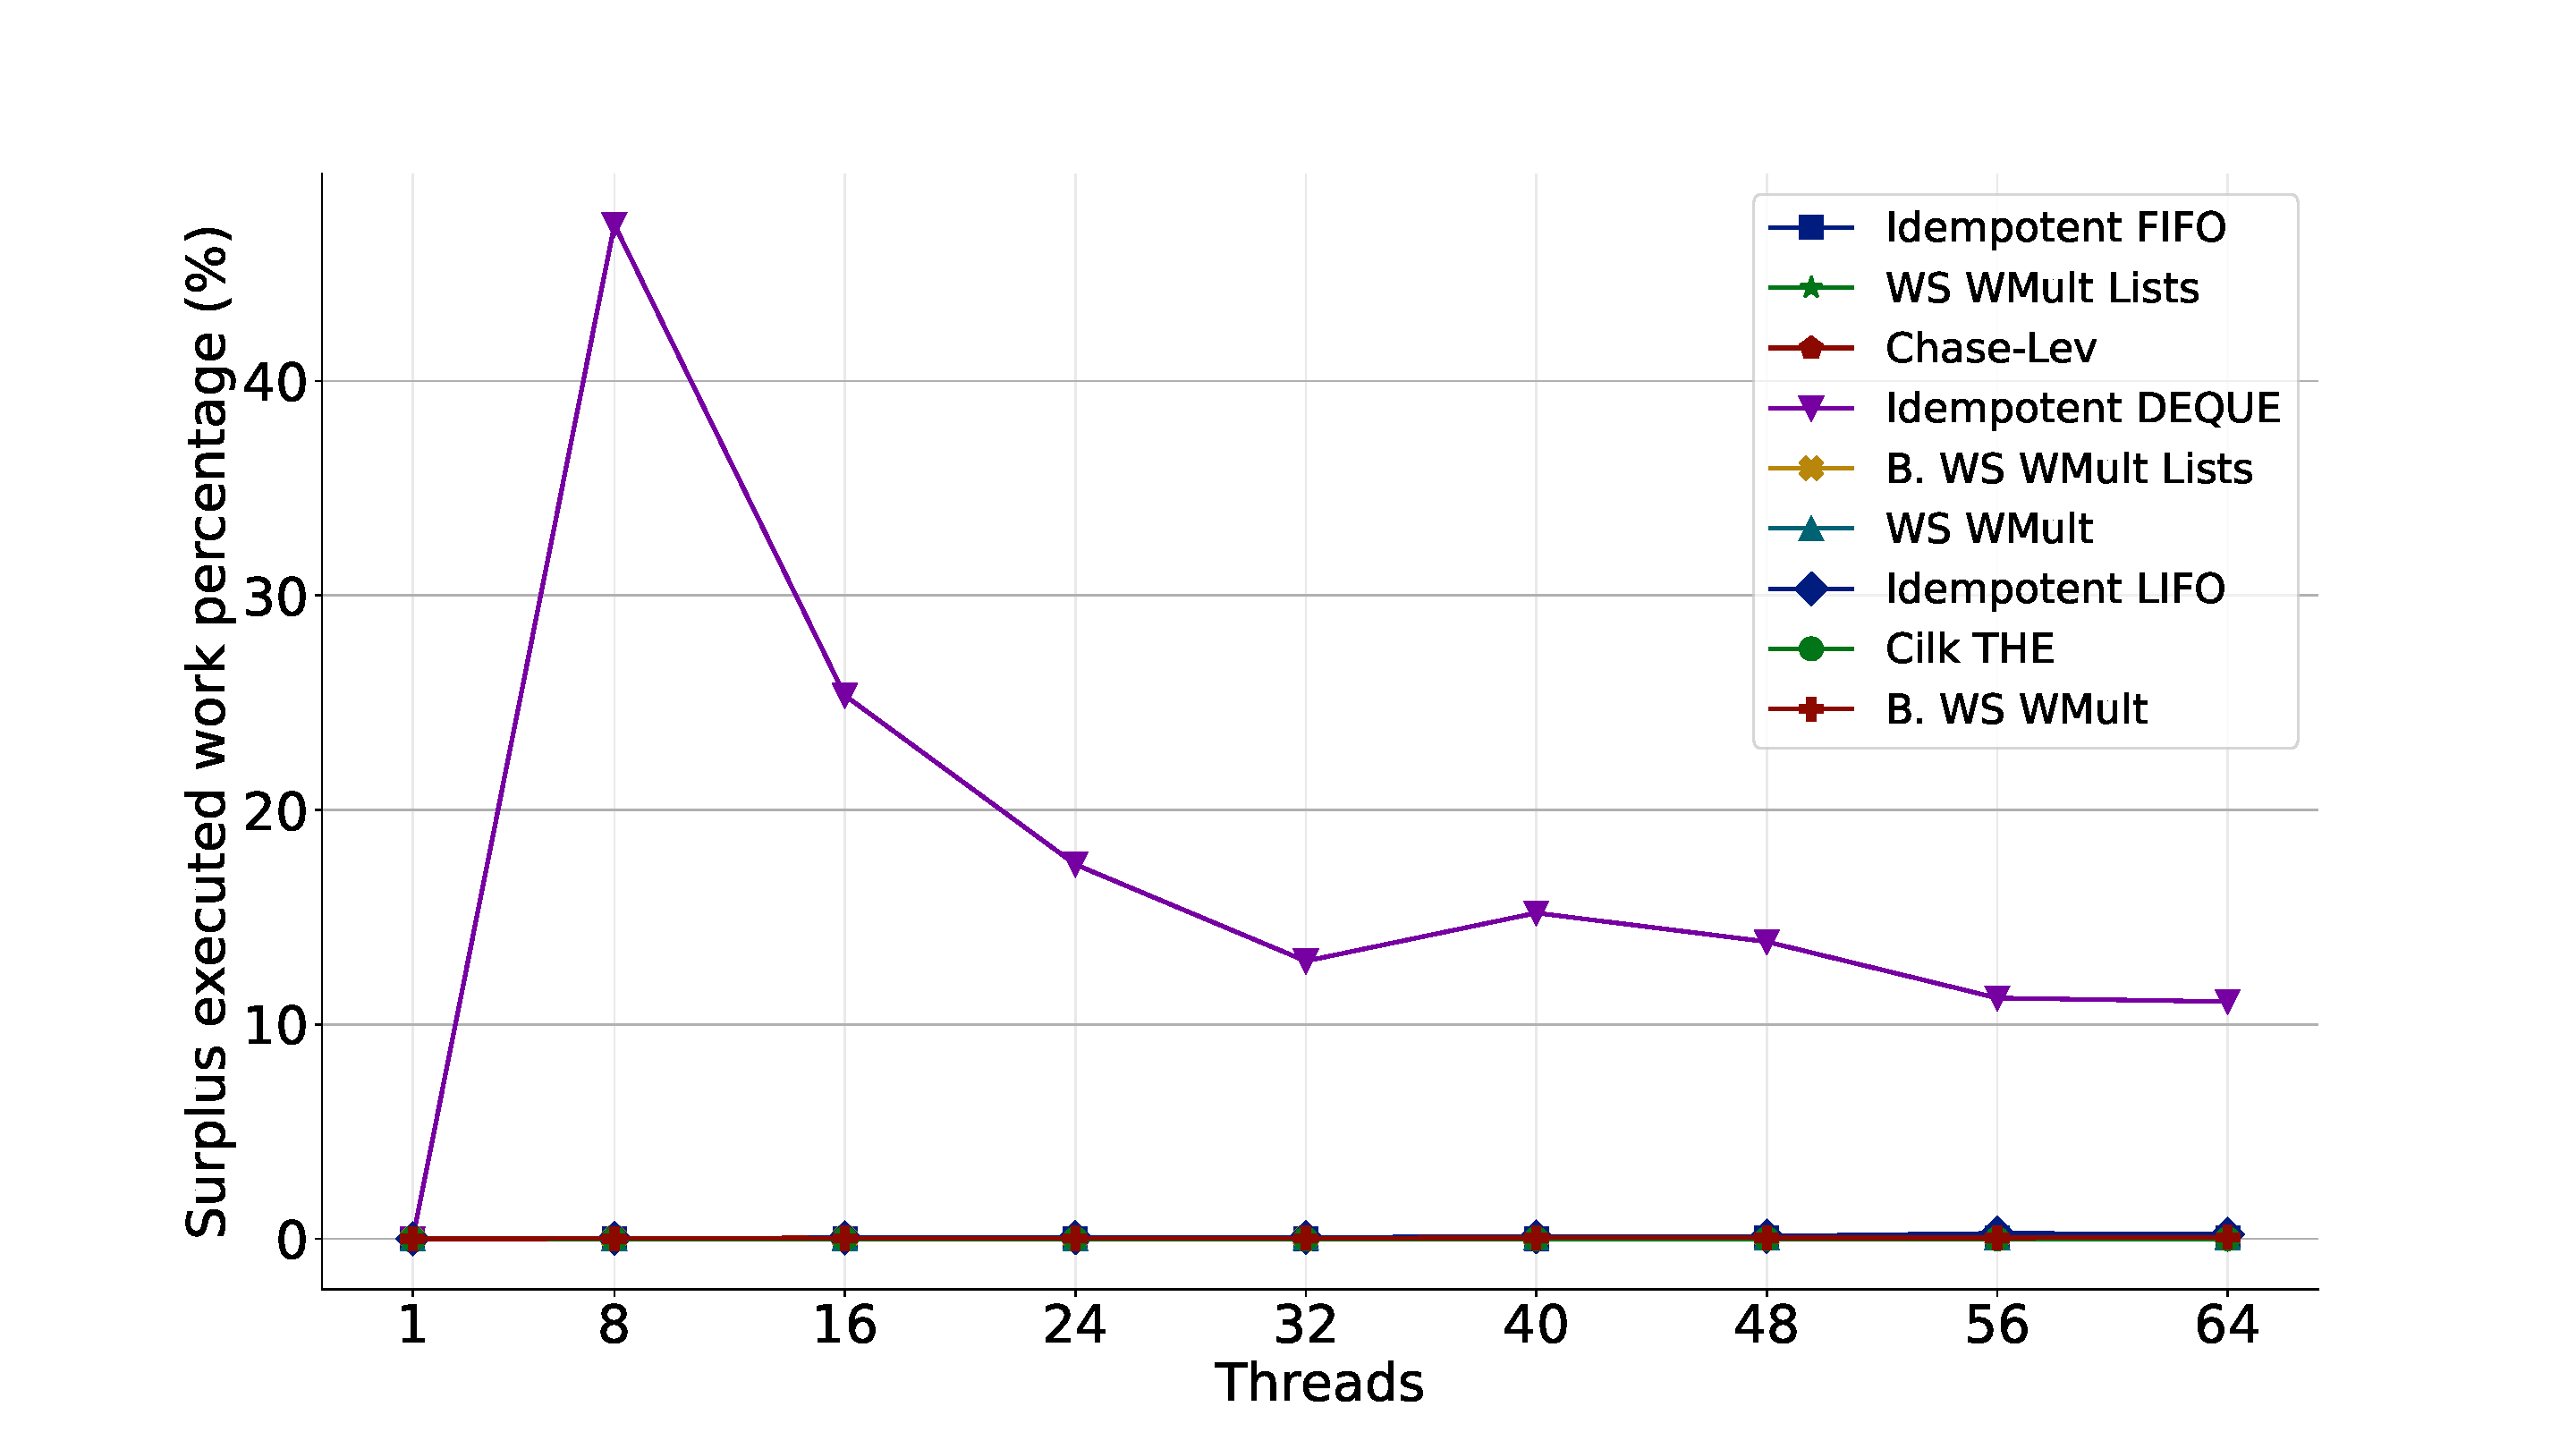
\includegraphics[width=0.48\textwidth]{contents/figures/IV_6_mult-exec-torus_2d_directed_1m.pdf}
  }

  \subfloat[\label{fig:exec-surplustorus3ddirected:256}Executed surplus work: Directed Torus 3D. Initial size of 256 items.]{
    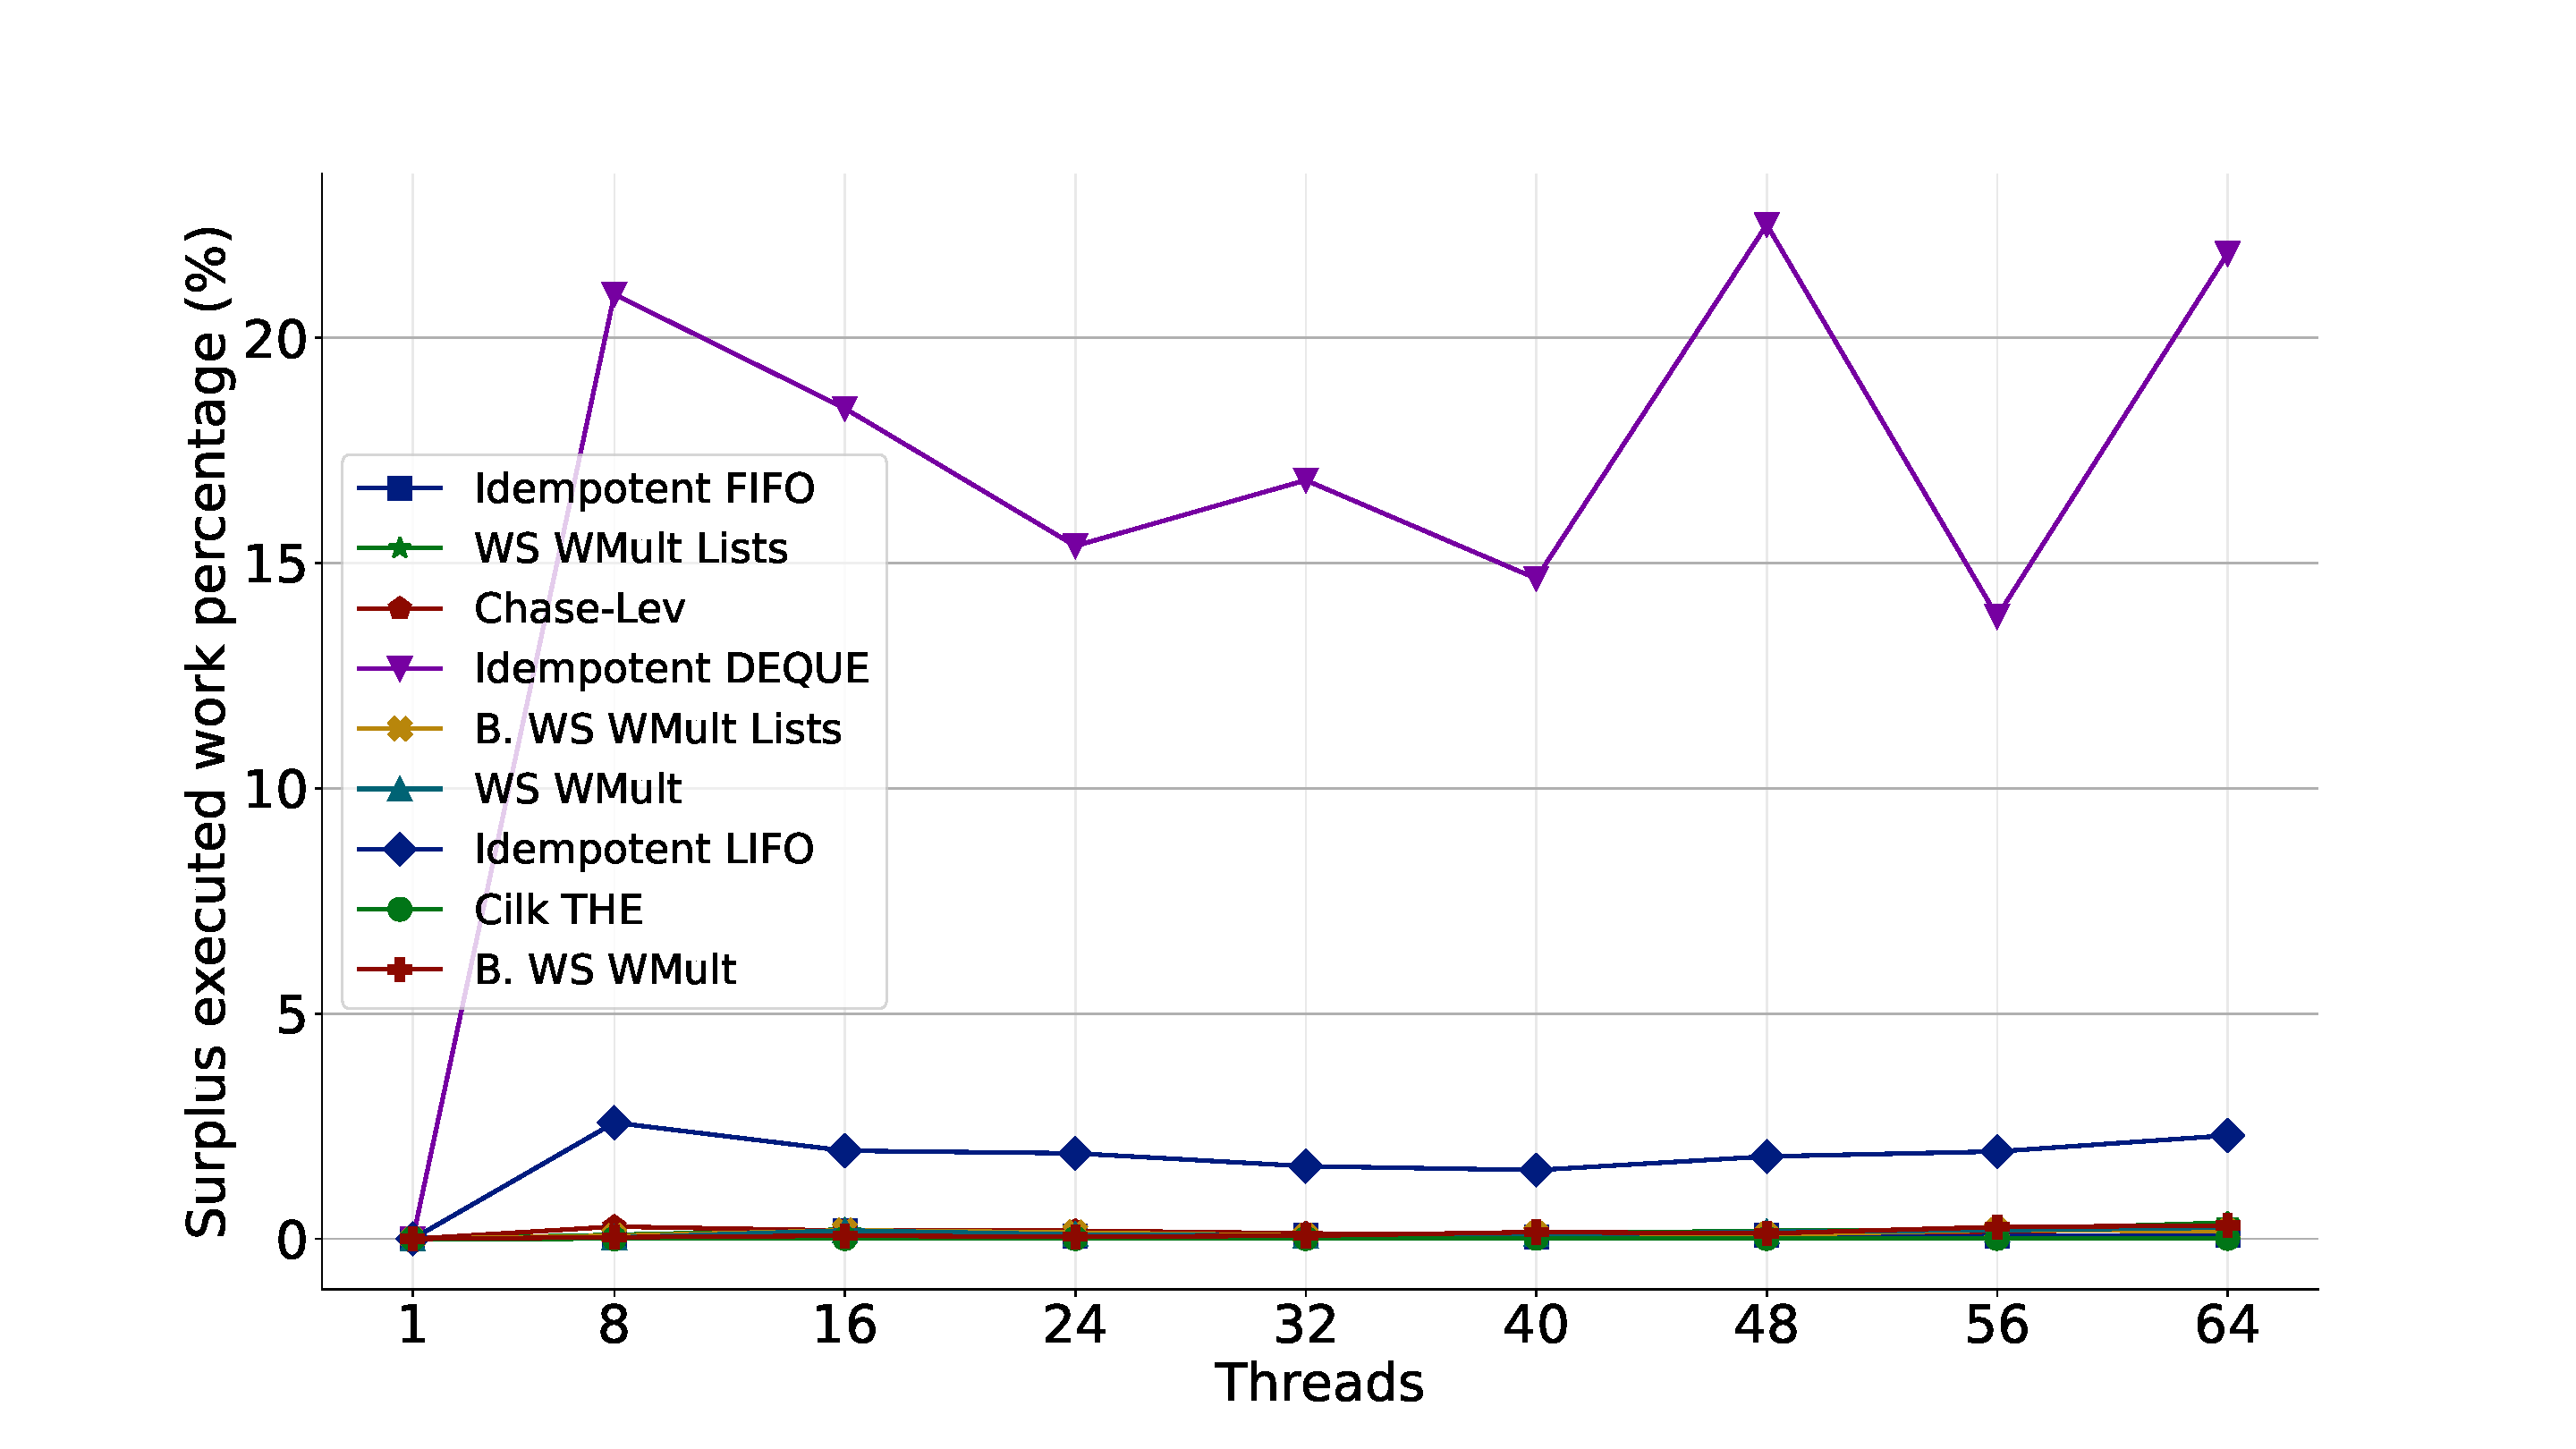
\includegraphics[width=0.48\textwidth]{contents/figures/IV_6_mult-exec-torus_3d_directed_256.pdf}
  }
  \subfloat[\label{fig:exec-surplustorus3ddirected:1000000}Executed surplus work: Directed Torus 3D. Initial size of 1,000,000 items.]{
    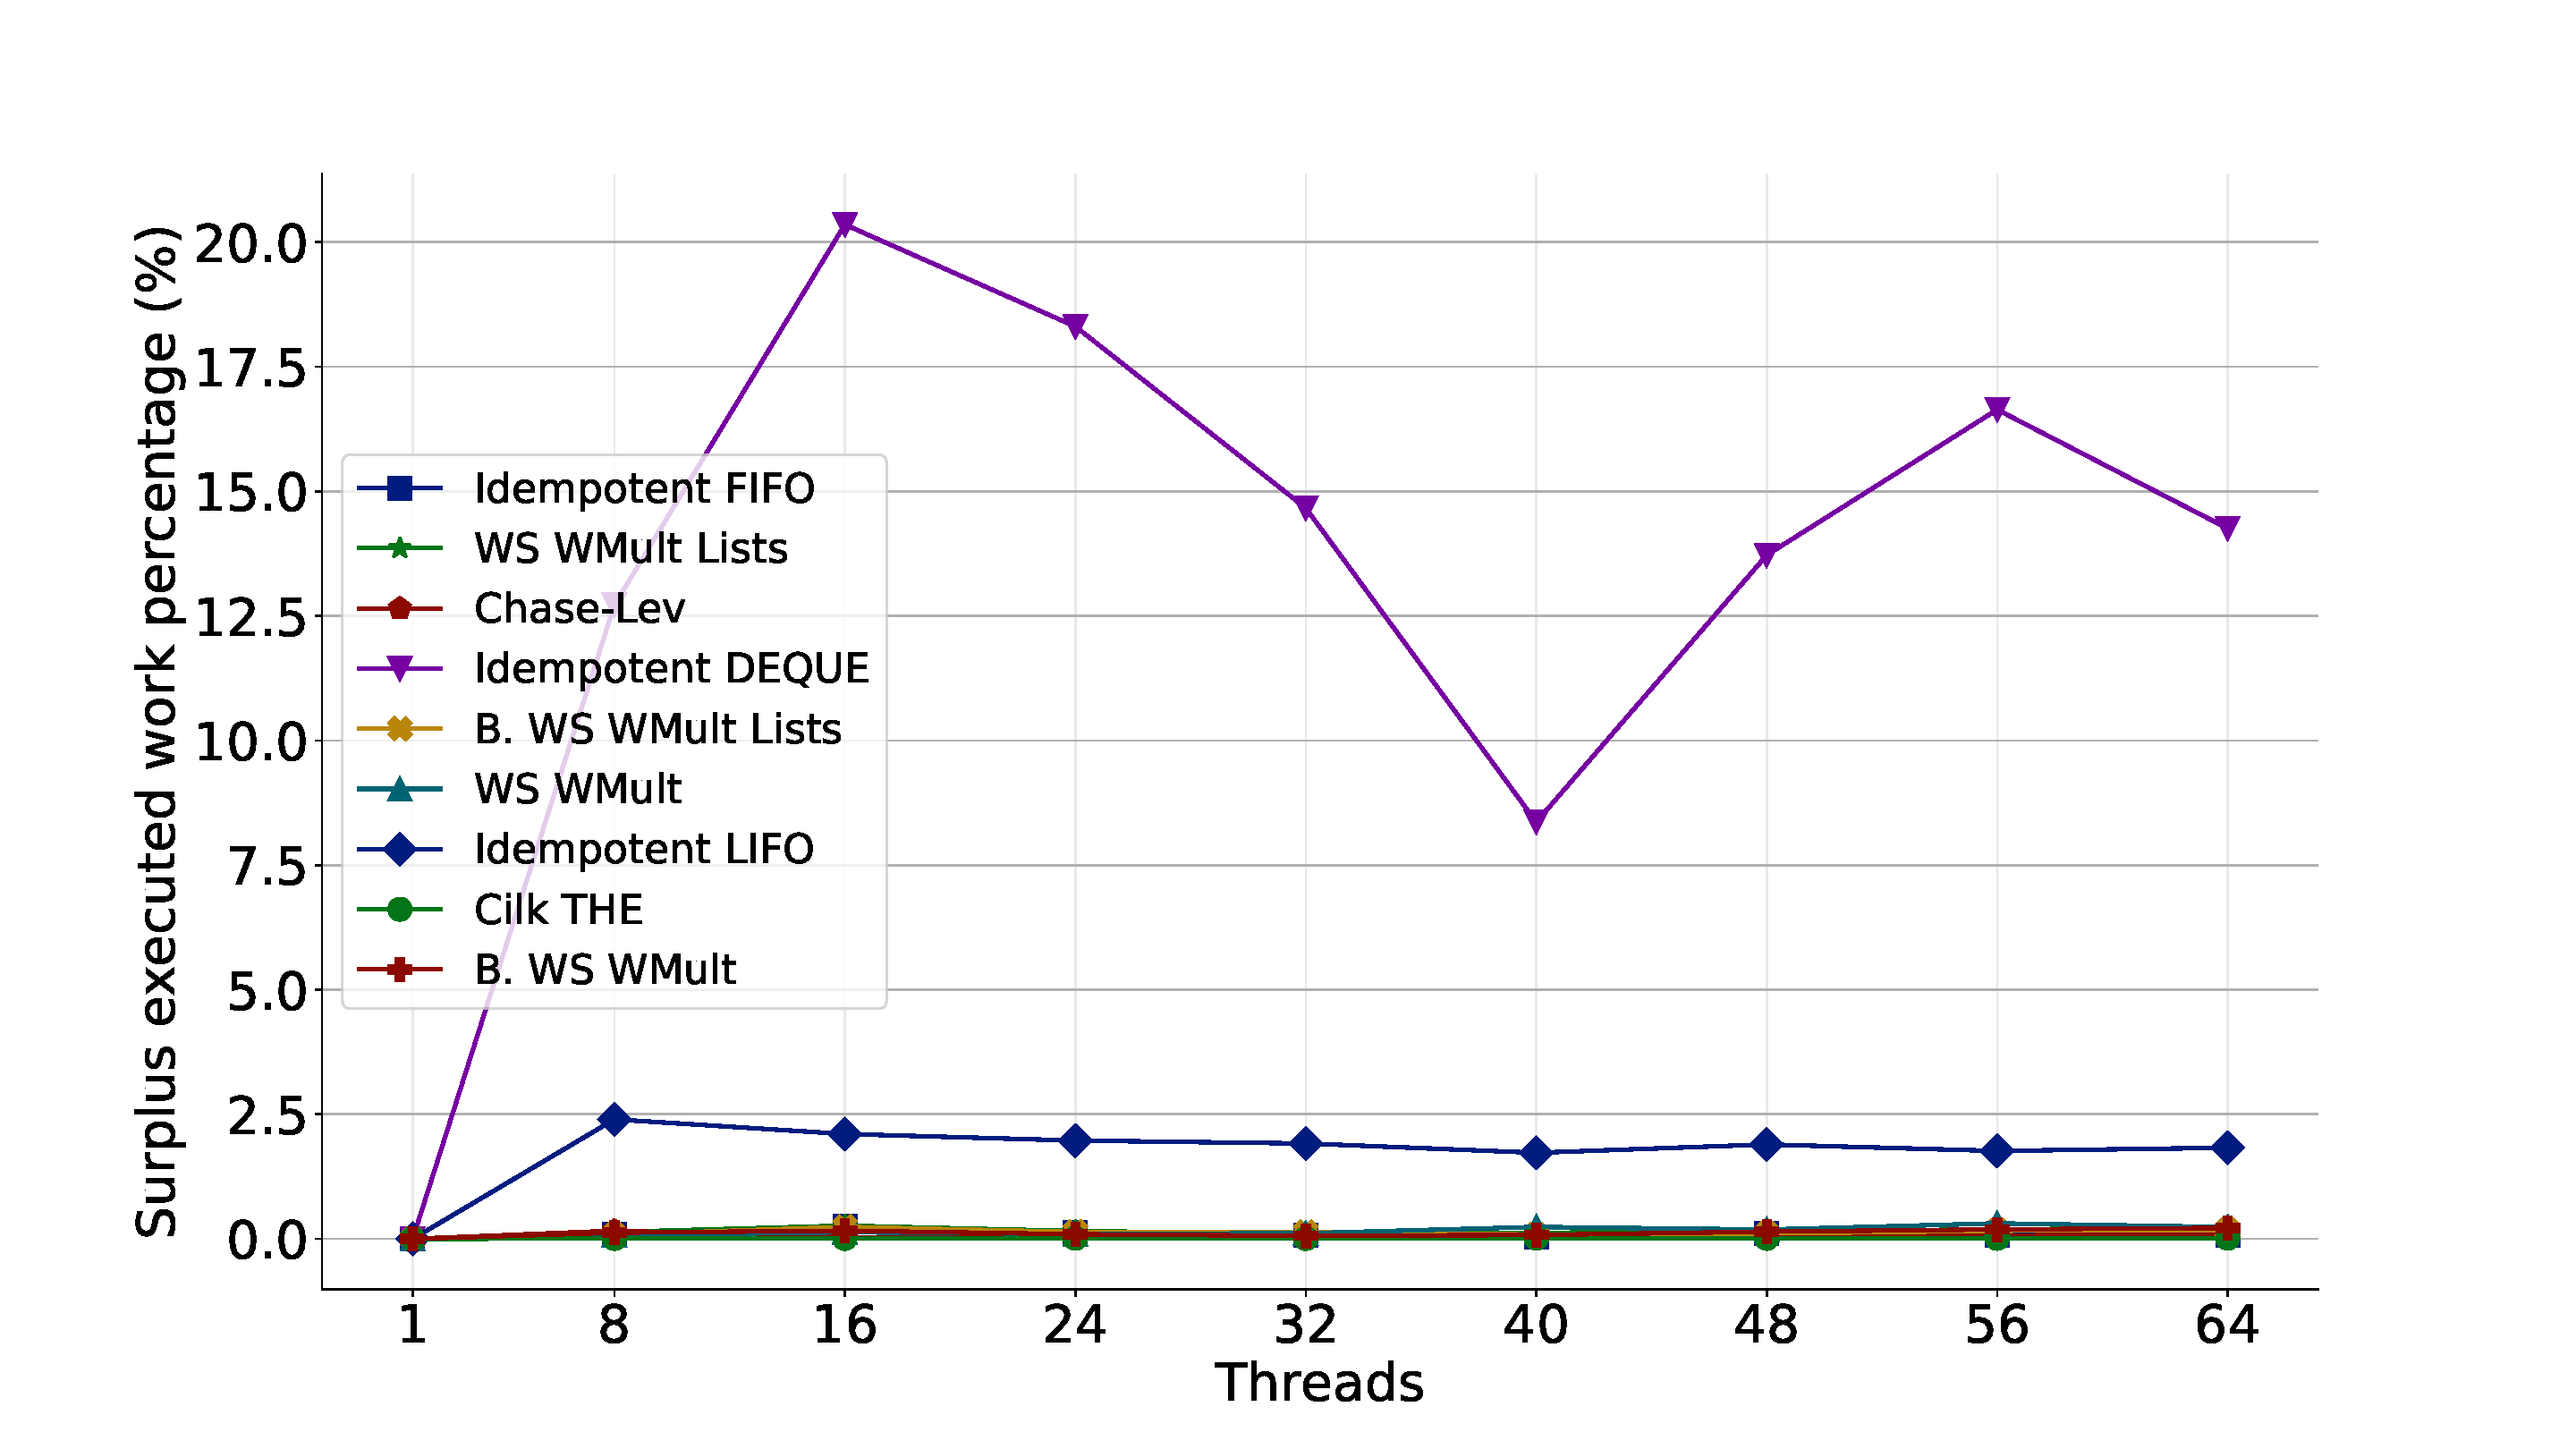
\includegraphics[width=0.48\textwidth]{contents/figures/IV_6_mult-exec-torus_3d_directed_1m.pdf}
  }

  \subfloat[\label{fig:exec-surplusrandom:256}Executed surplus work: Directed Random. Initial size of 256 items.]{
    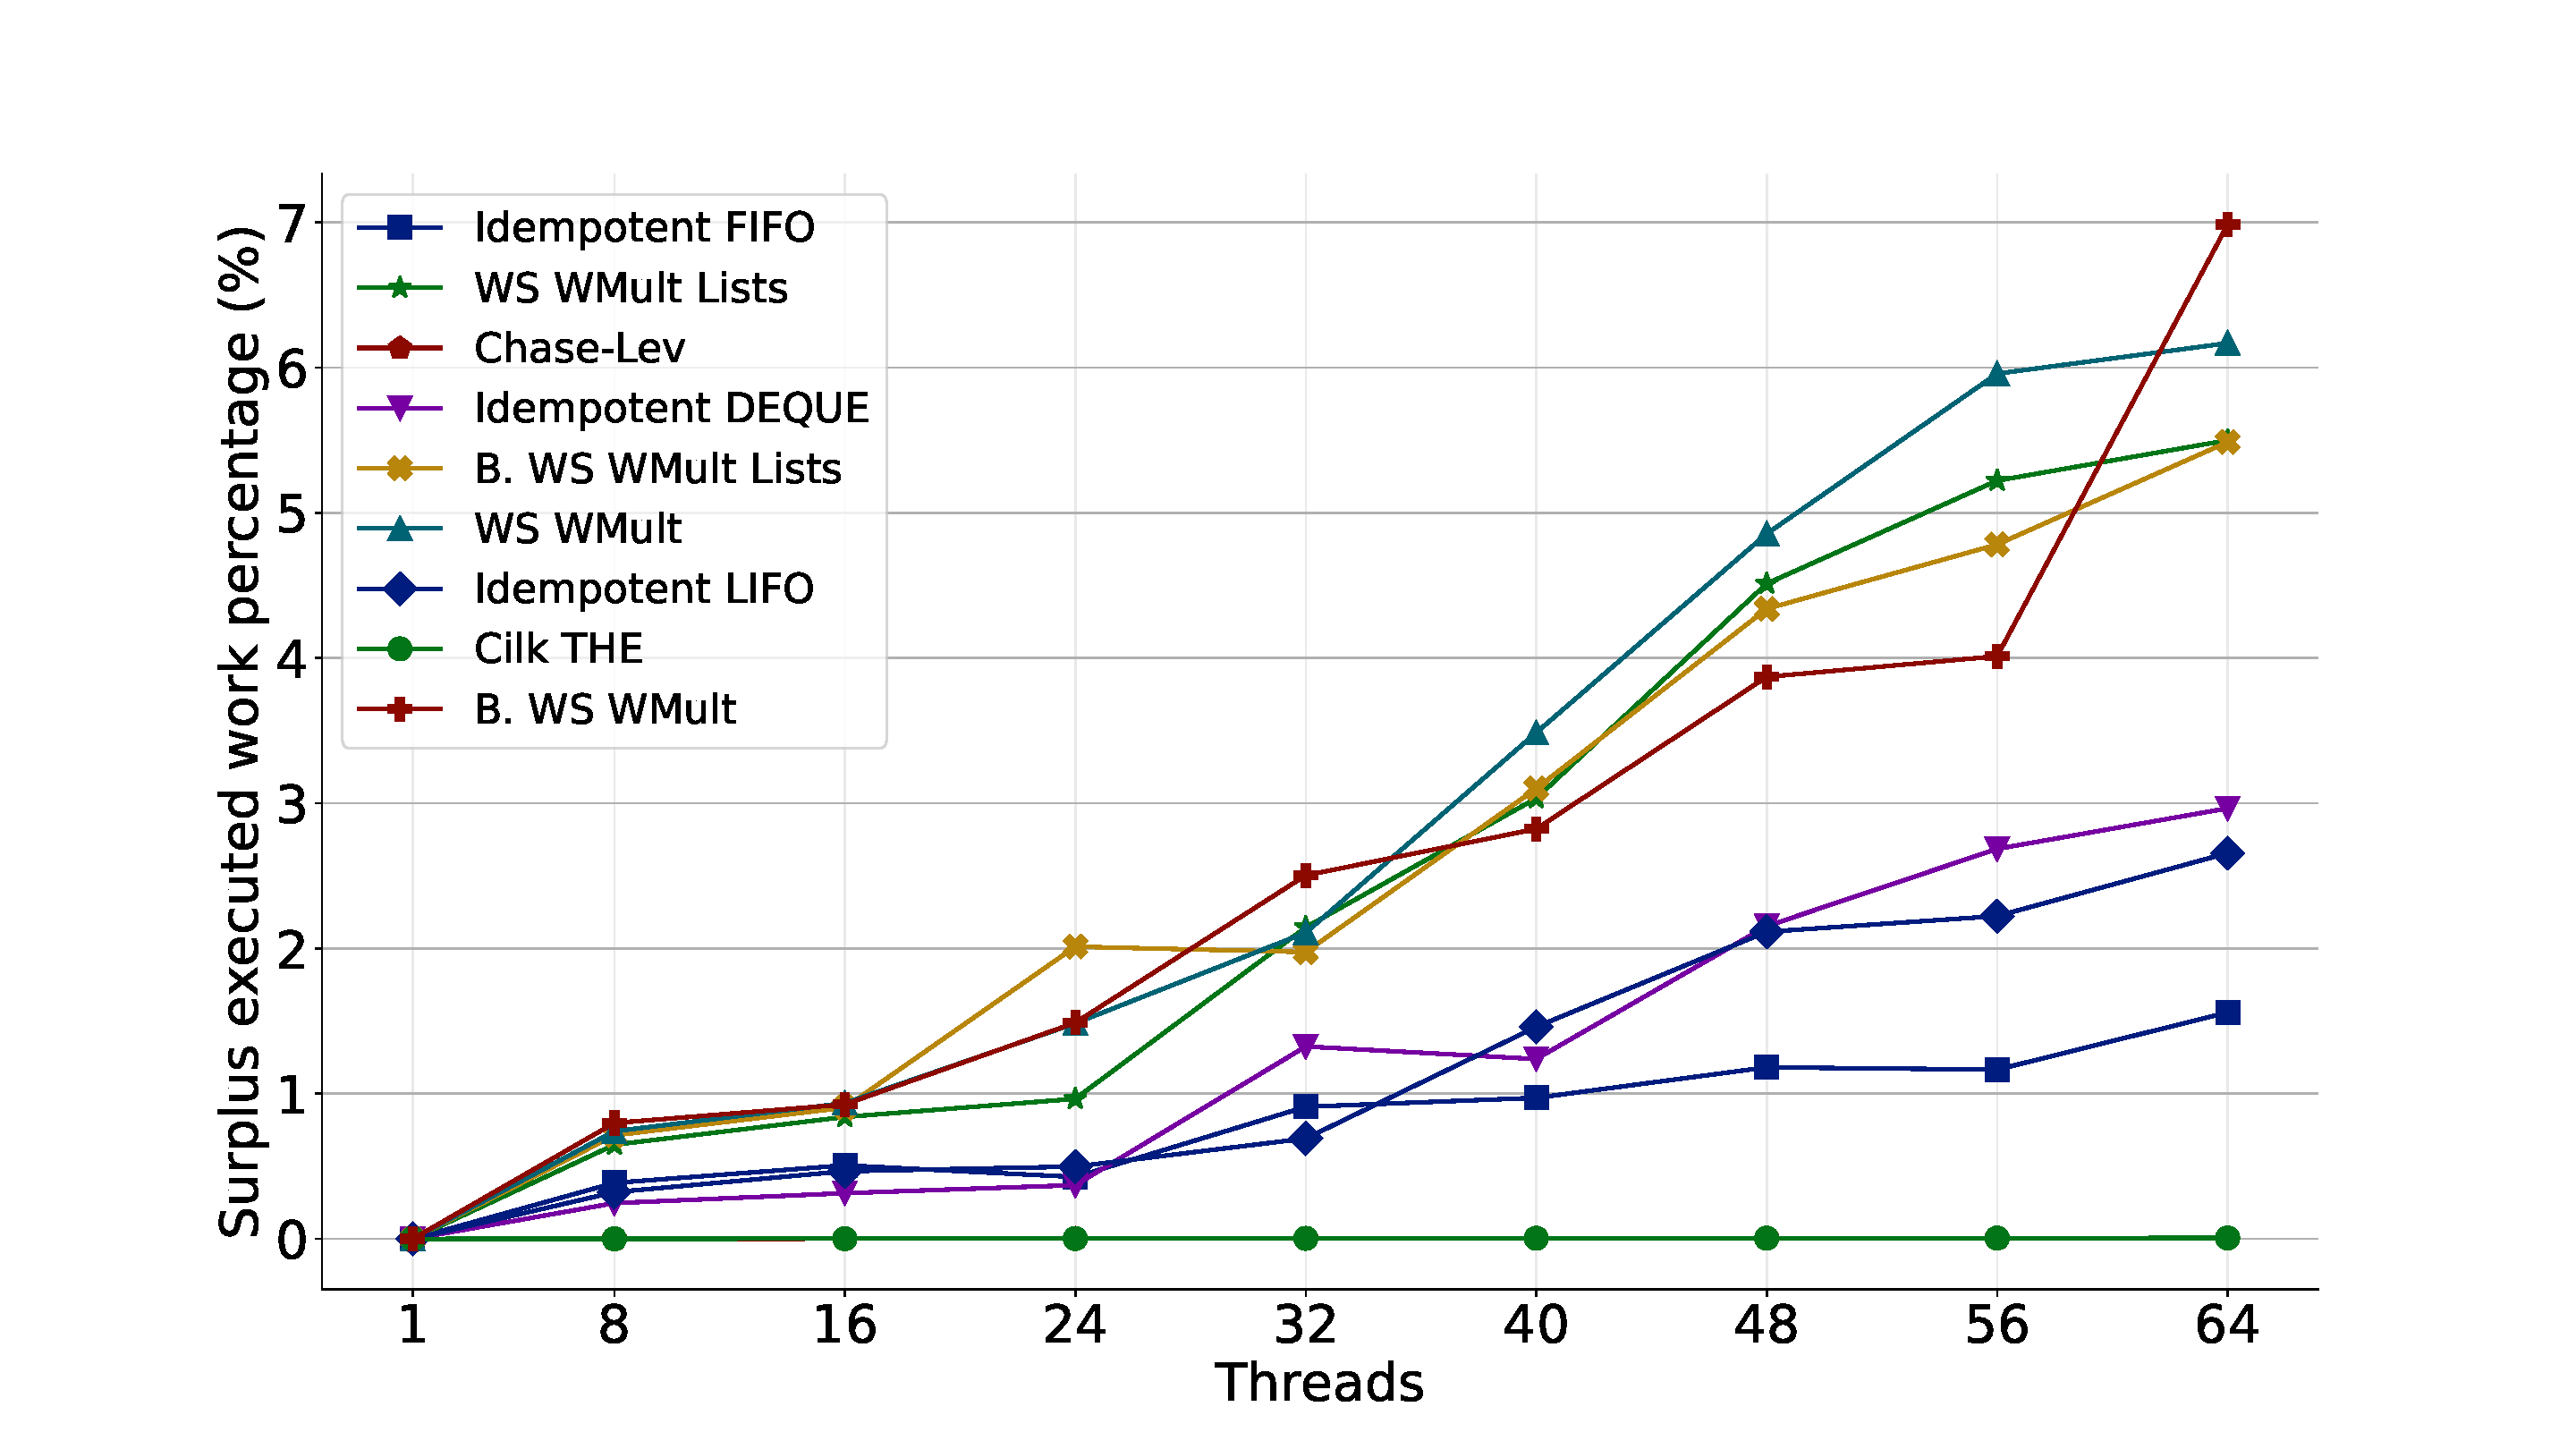
\includegraphics[width=0.48\textwidth]{contents/figures/IV_6_mult-exec-random_directed_256.pdf}
  }
  \subfloat[\label{fig:exec-surplusrandom:1000000}Executed surplus work: Directed Random: Initial size of 1,000,000 items.]{
    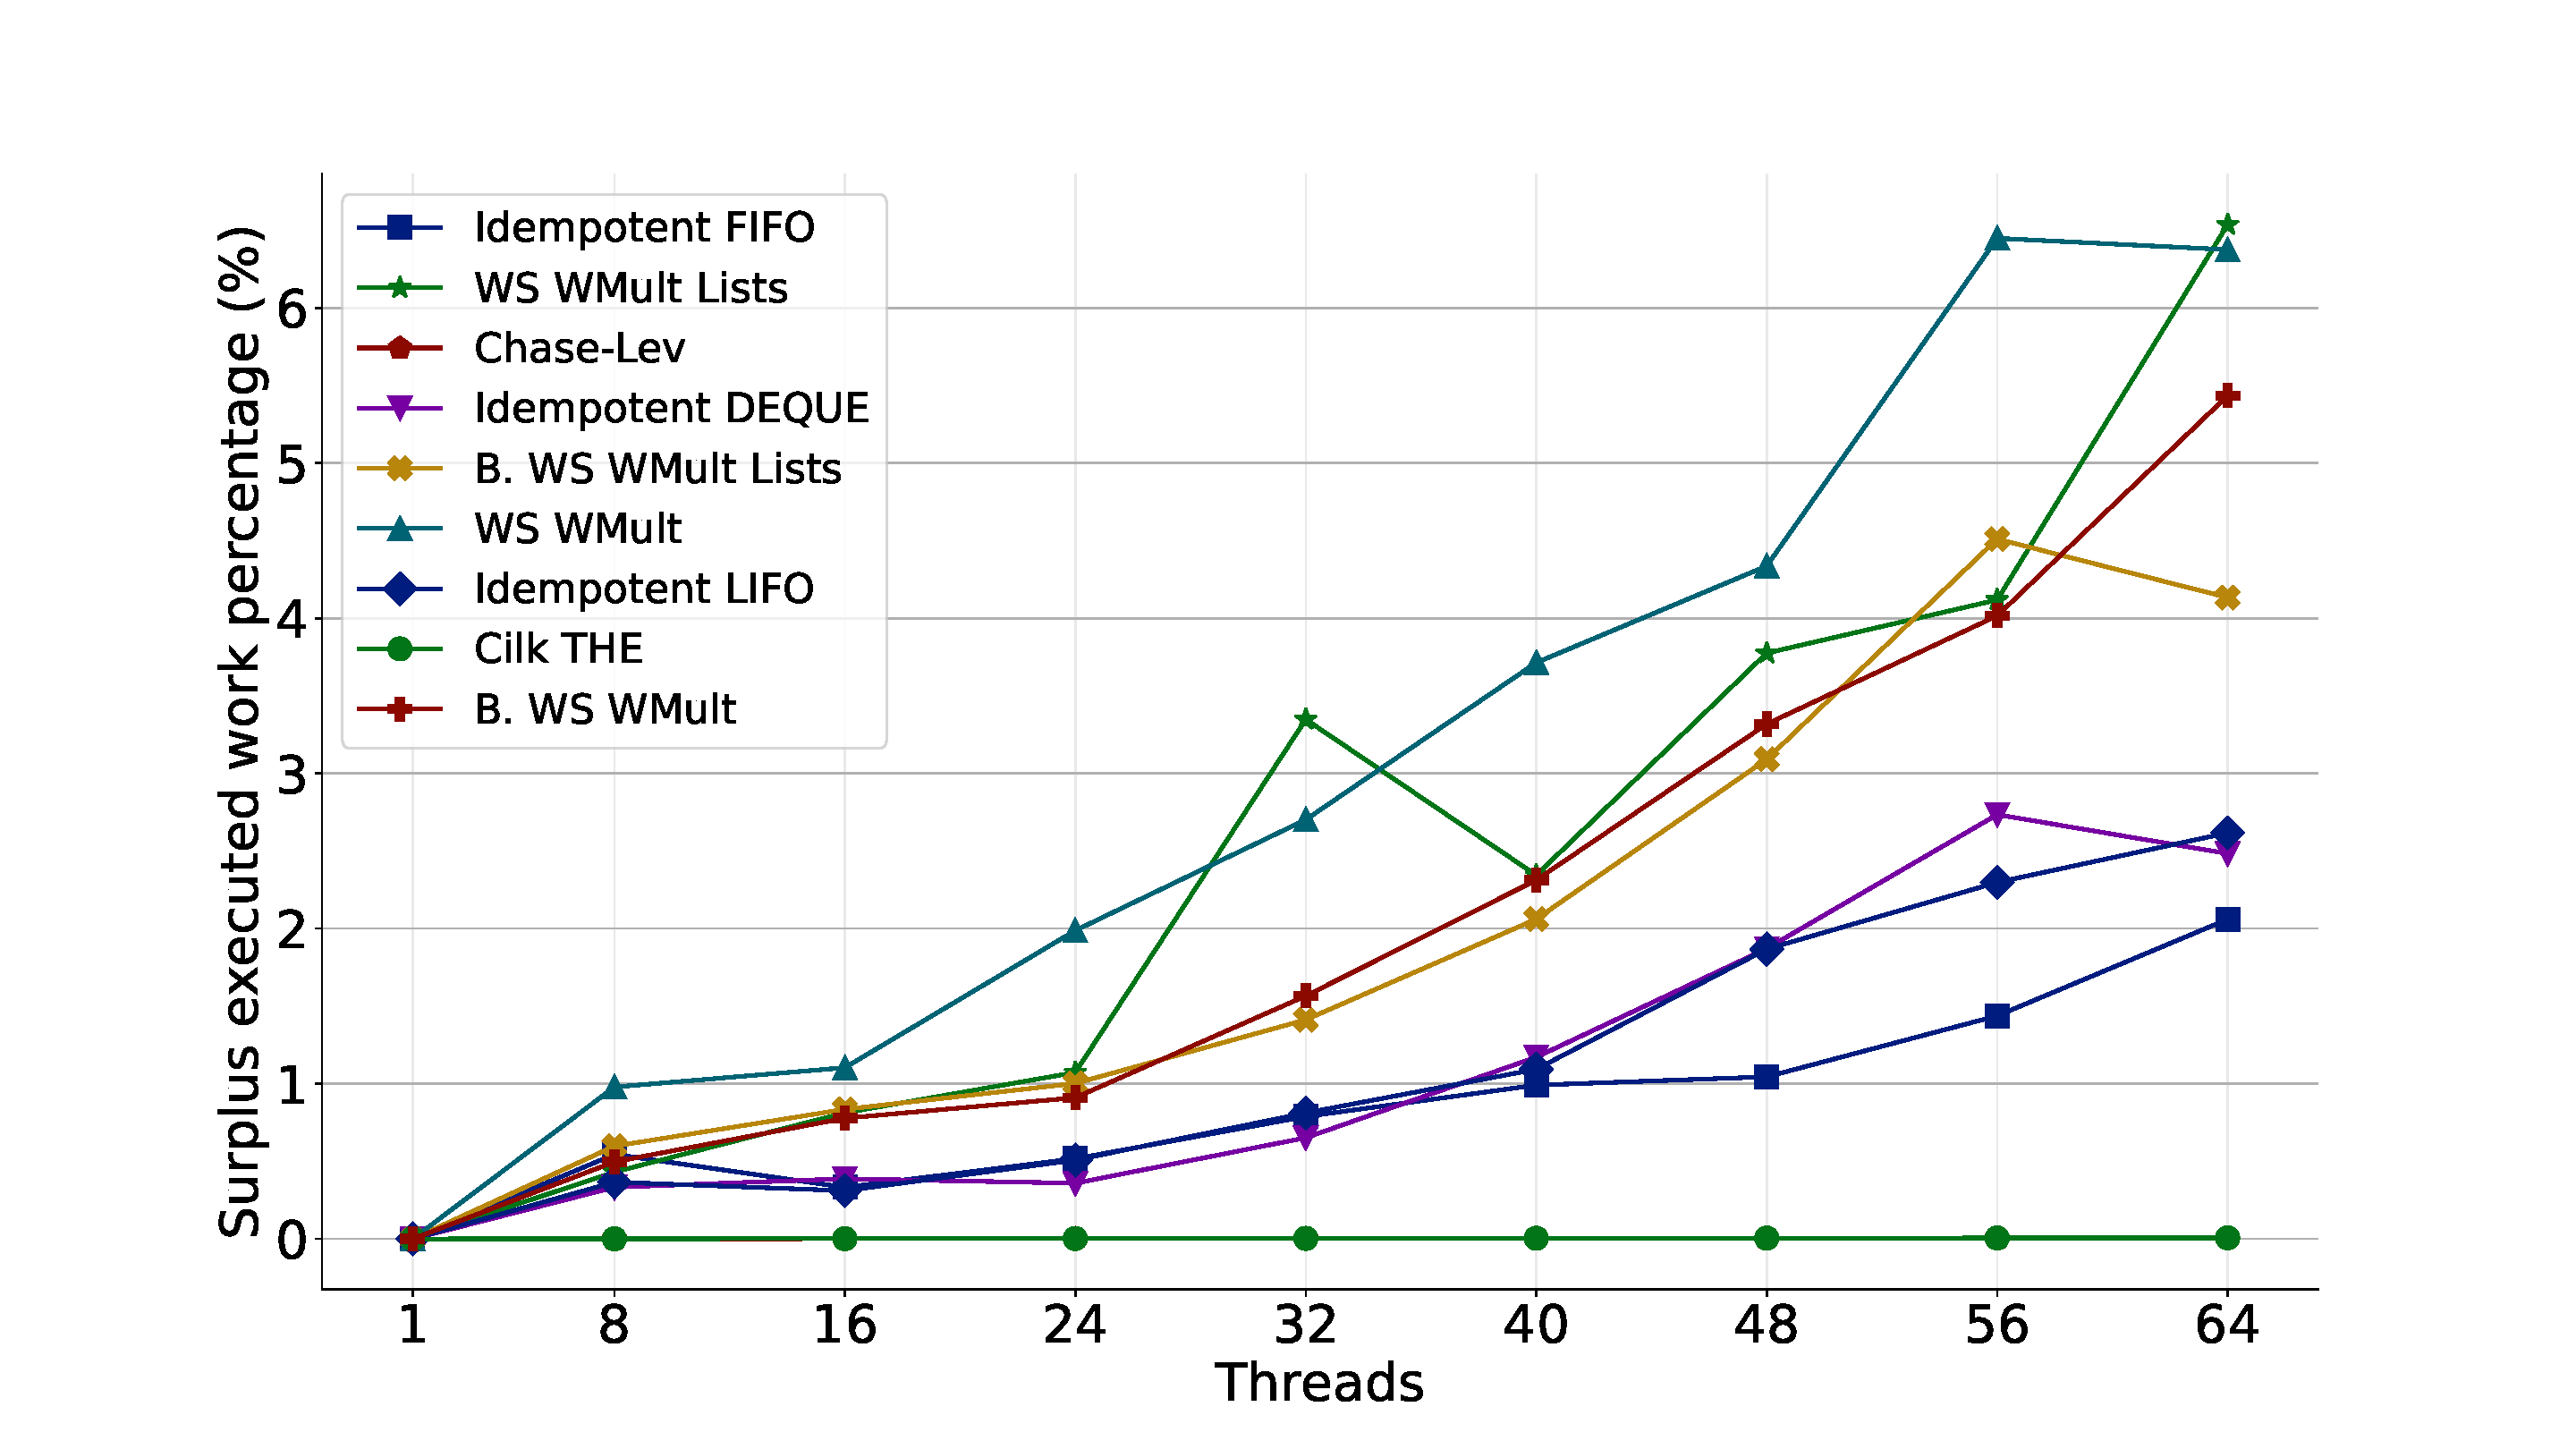
\includegraphics[width=0.48\textwidth]{contents/figures/IV_6_mult-exec-random_directed_1m.pdf}
  }

  \caption{\label{fig:exec-surplusgraphapplication} Executed surplus work (percentage) of the experiments. Surplus work: the difference between the total number of \Takes, and the number of takes in sequential executions (i.e., $1,000,000$).}

\end{figure}

\begin{figure}[!ht]
  \subfloat[\label{fig:sat:50:1}Range assignment size 50.]{
    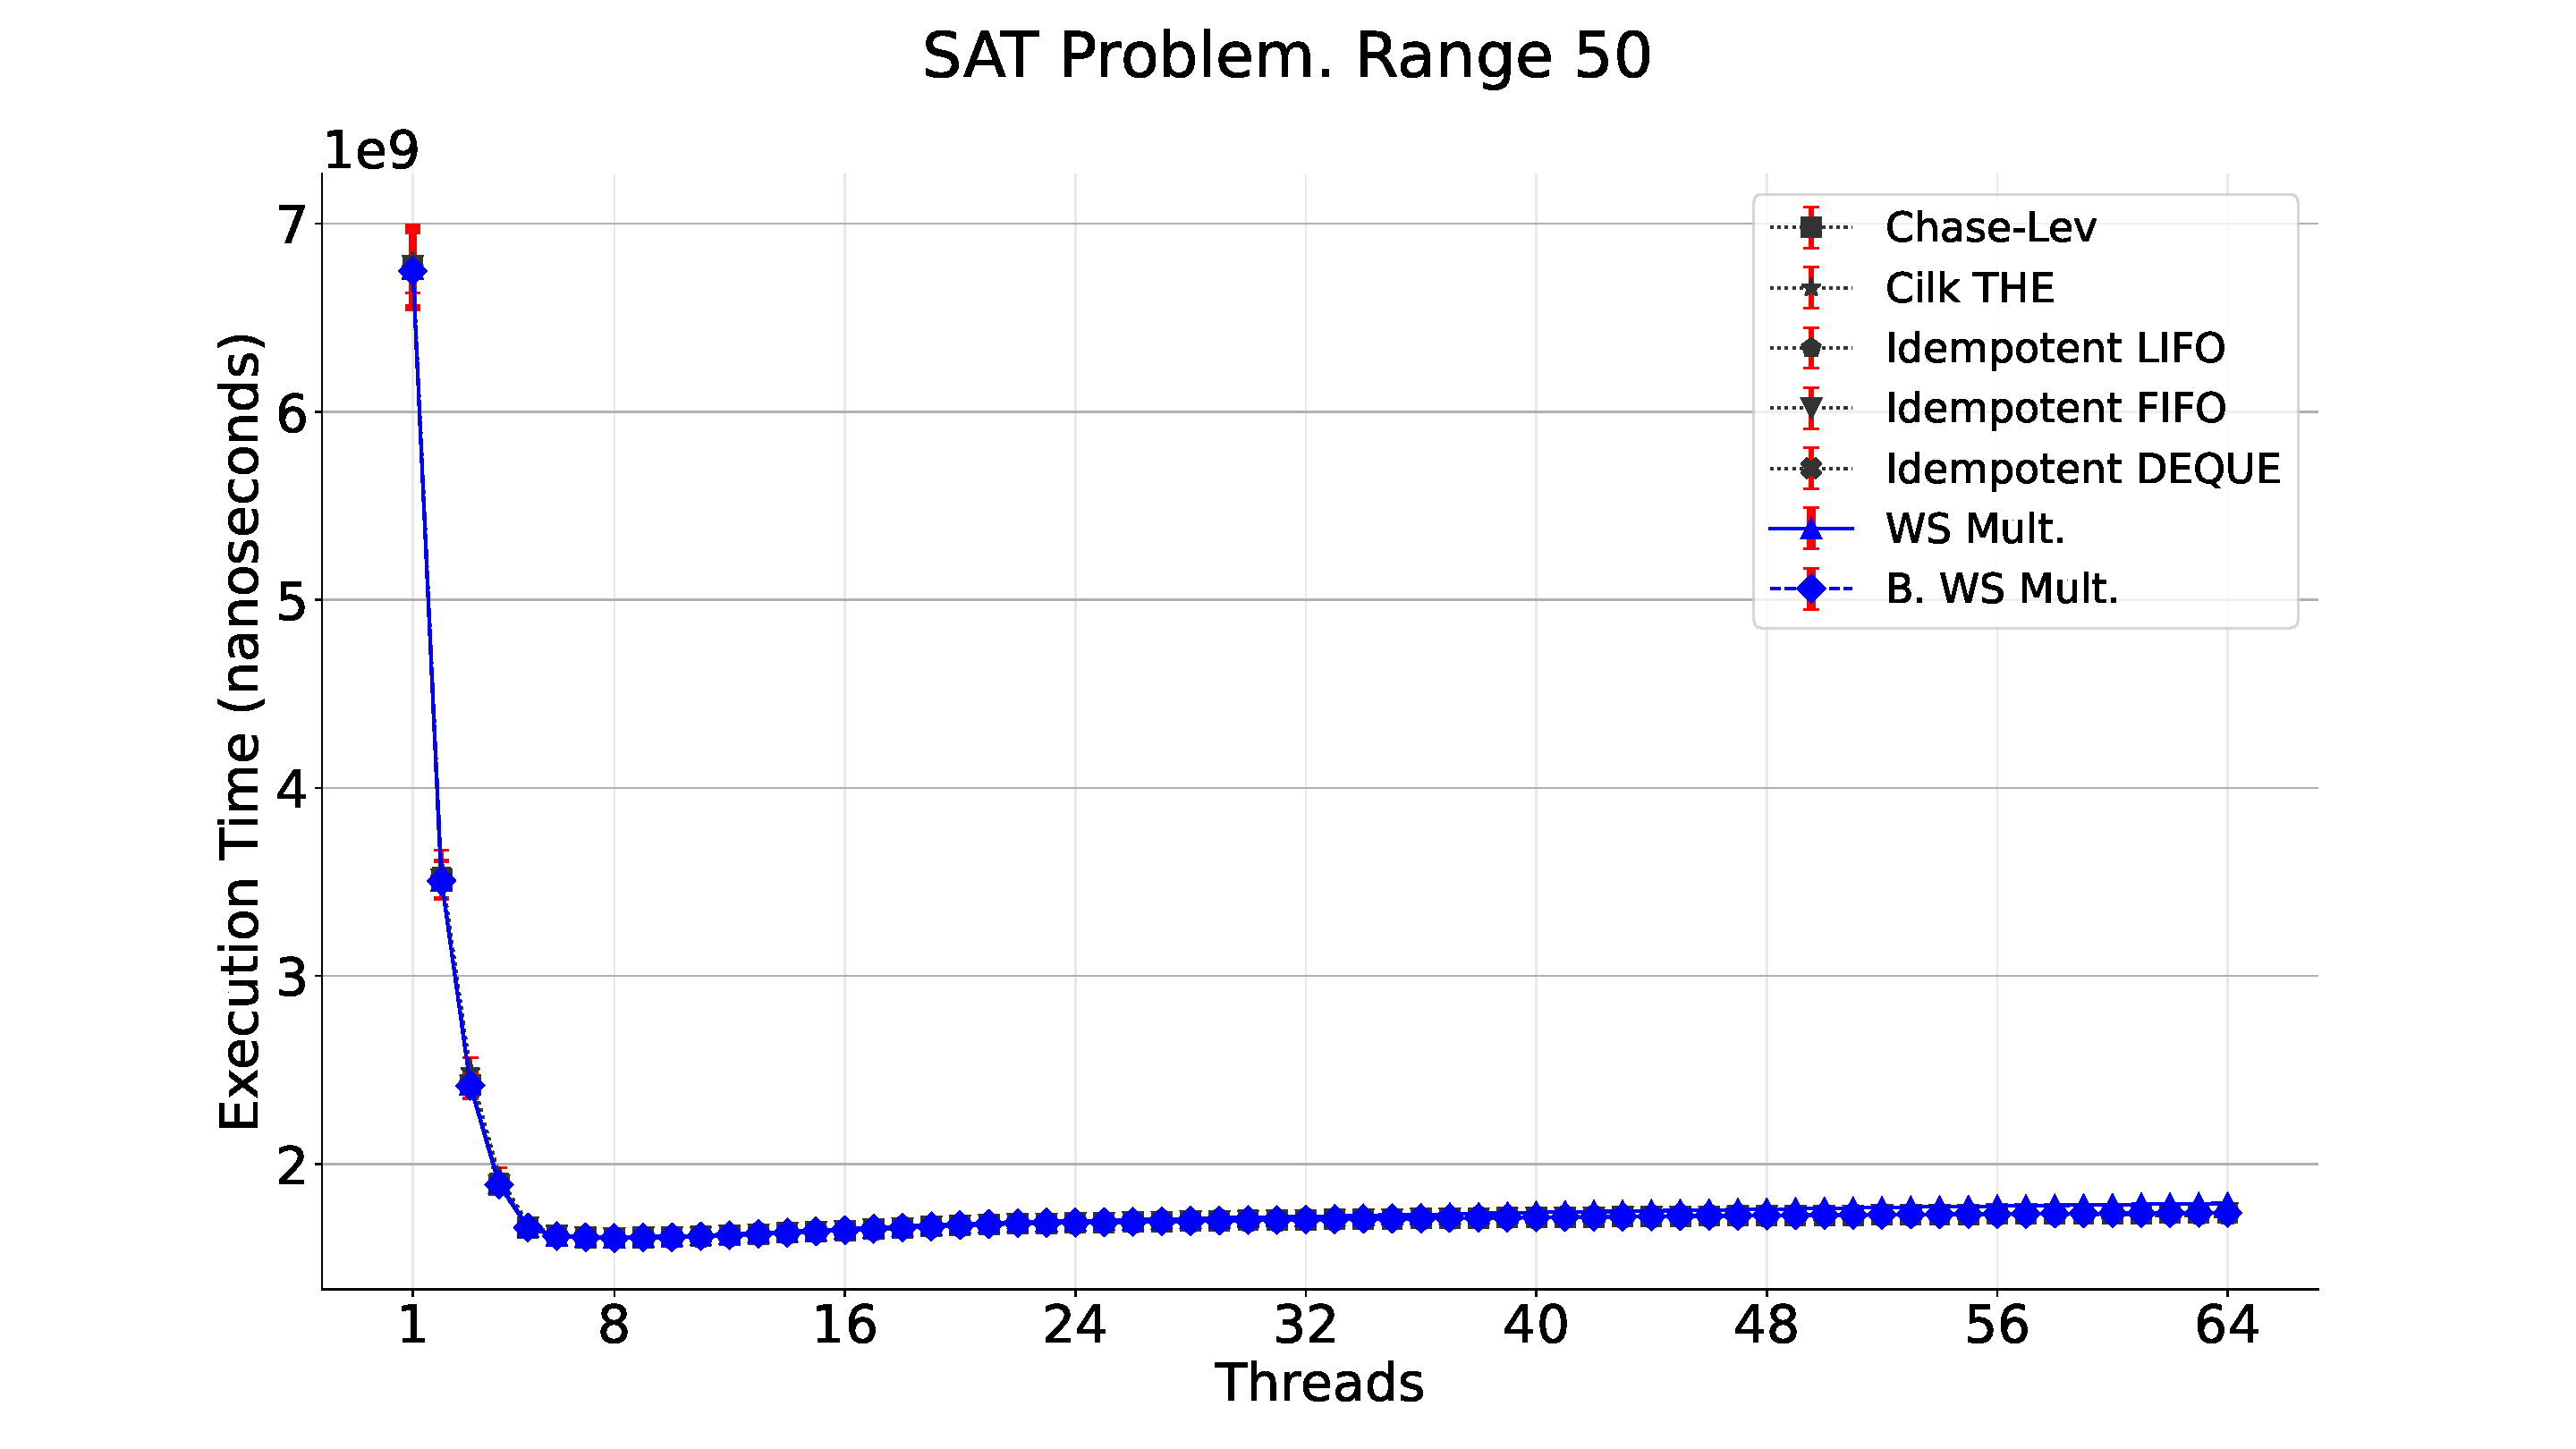
\includegraphics[width=0.48\textwidth]{contents/figures/IV_6_sat-50-1.pdf}
  }
  \subfloat[\label{fig:sat:50:2}Range assignment size 50. Zoom in to the number of processes 32 to 64.]{
    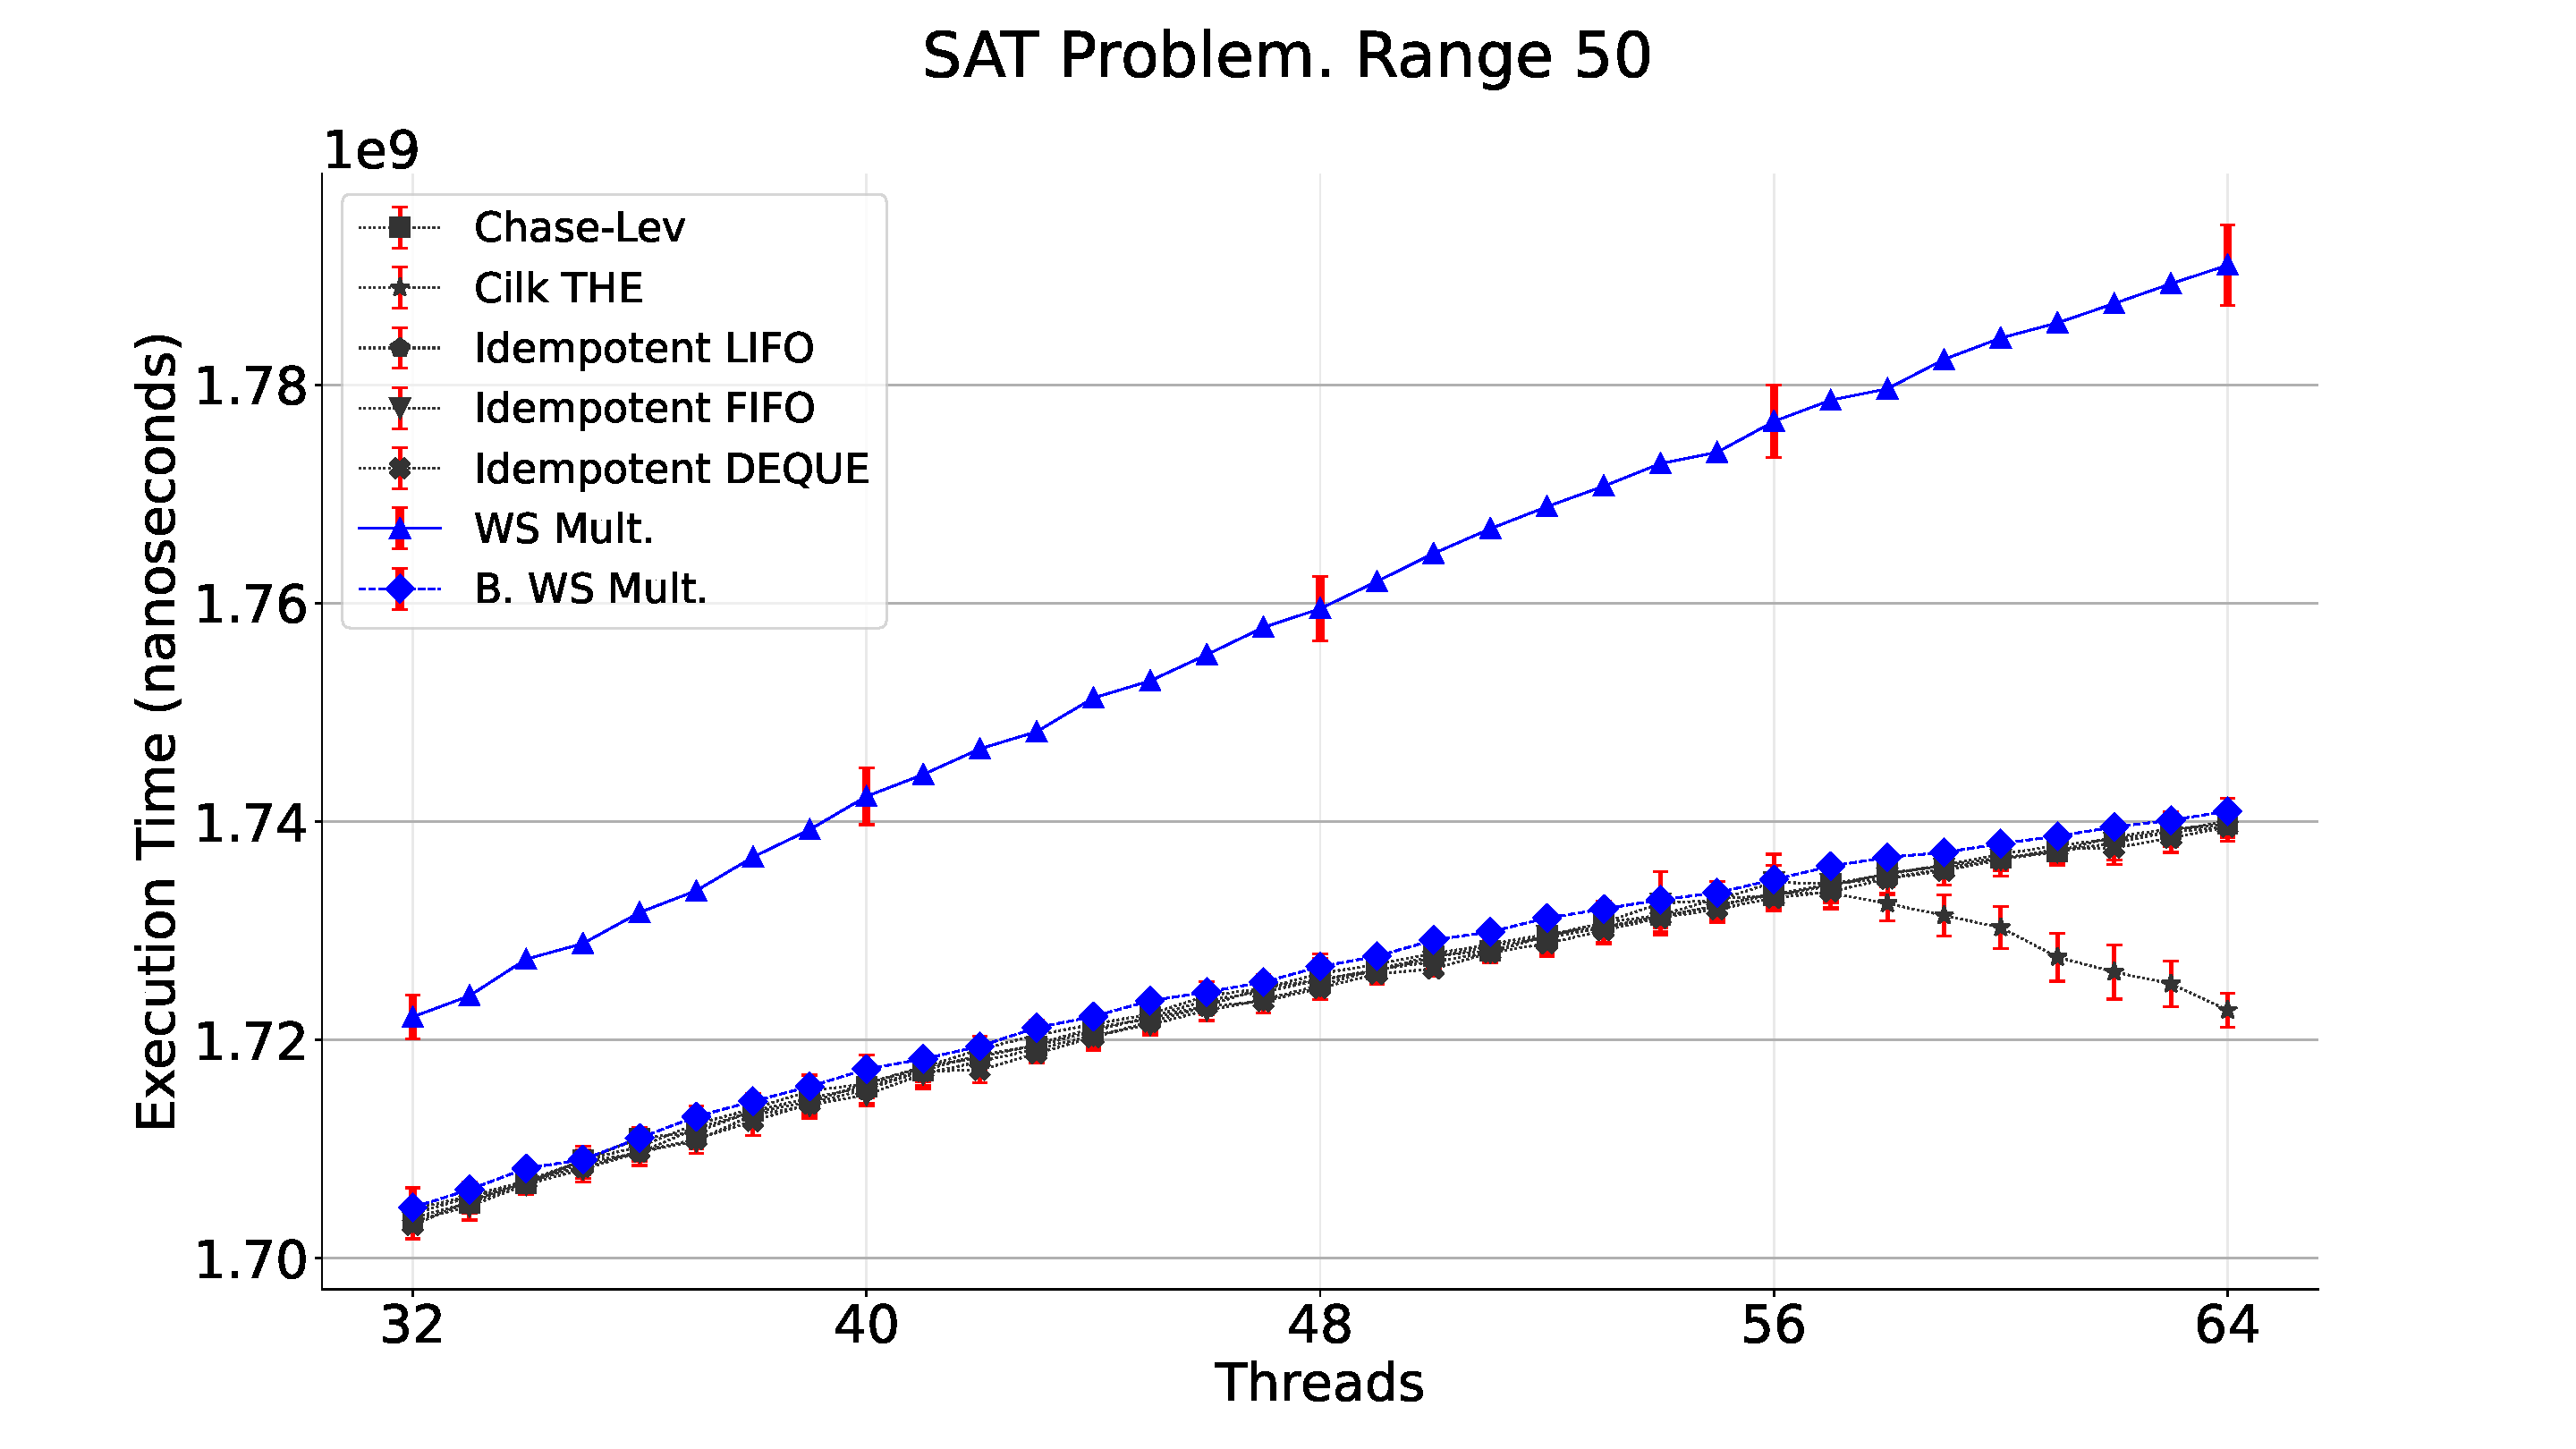
\includegraphics[width=0.48\textwidth]{contents/figures/IV_6_sat-50-2.pdf}
  }

  \subfloat[\label{fig:sat:250:1}Range assignment size 250.]{
    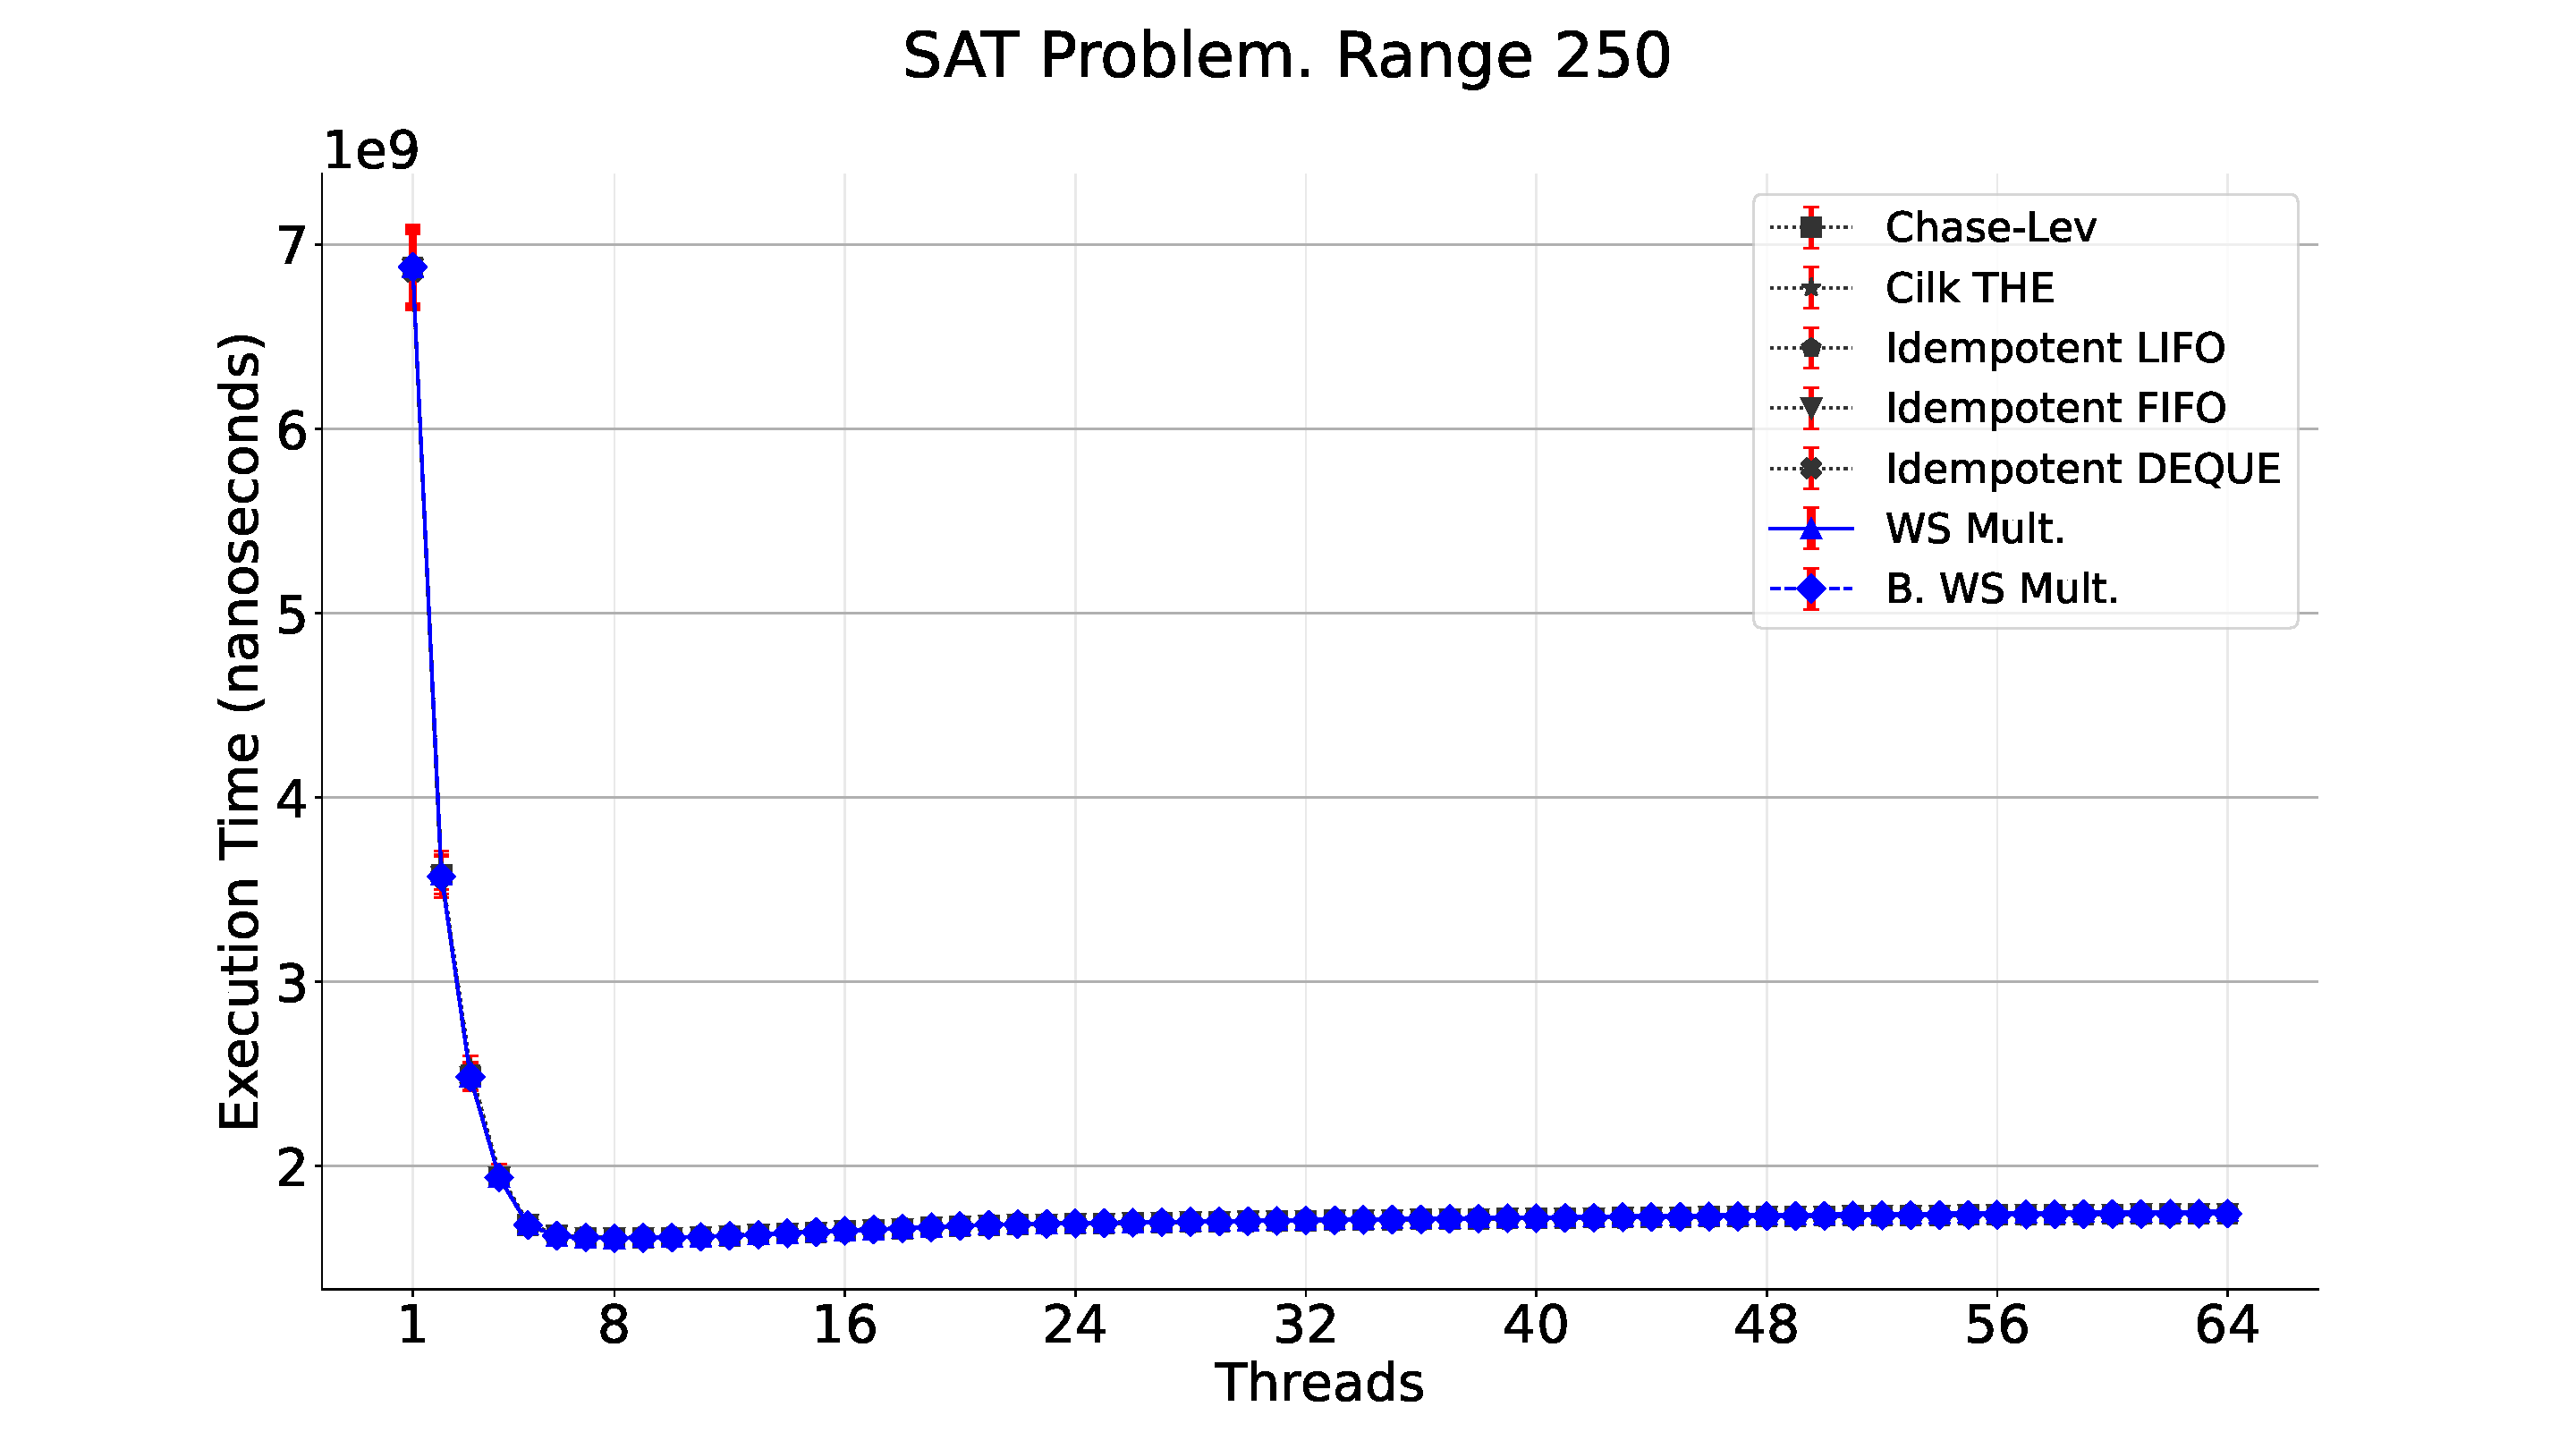
\includegraphics[width=0.48\textwidth]{contents/figures/IV_6_sat-250-1.pdf}
  }
  \subfloat[\label{fig:sat:250:2}Range assignment size 250. Zoom in to the number of processes 32 to 64.]{
    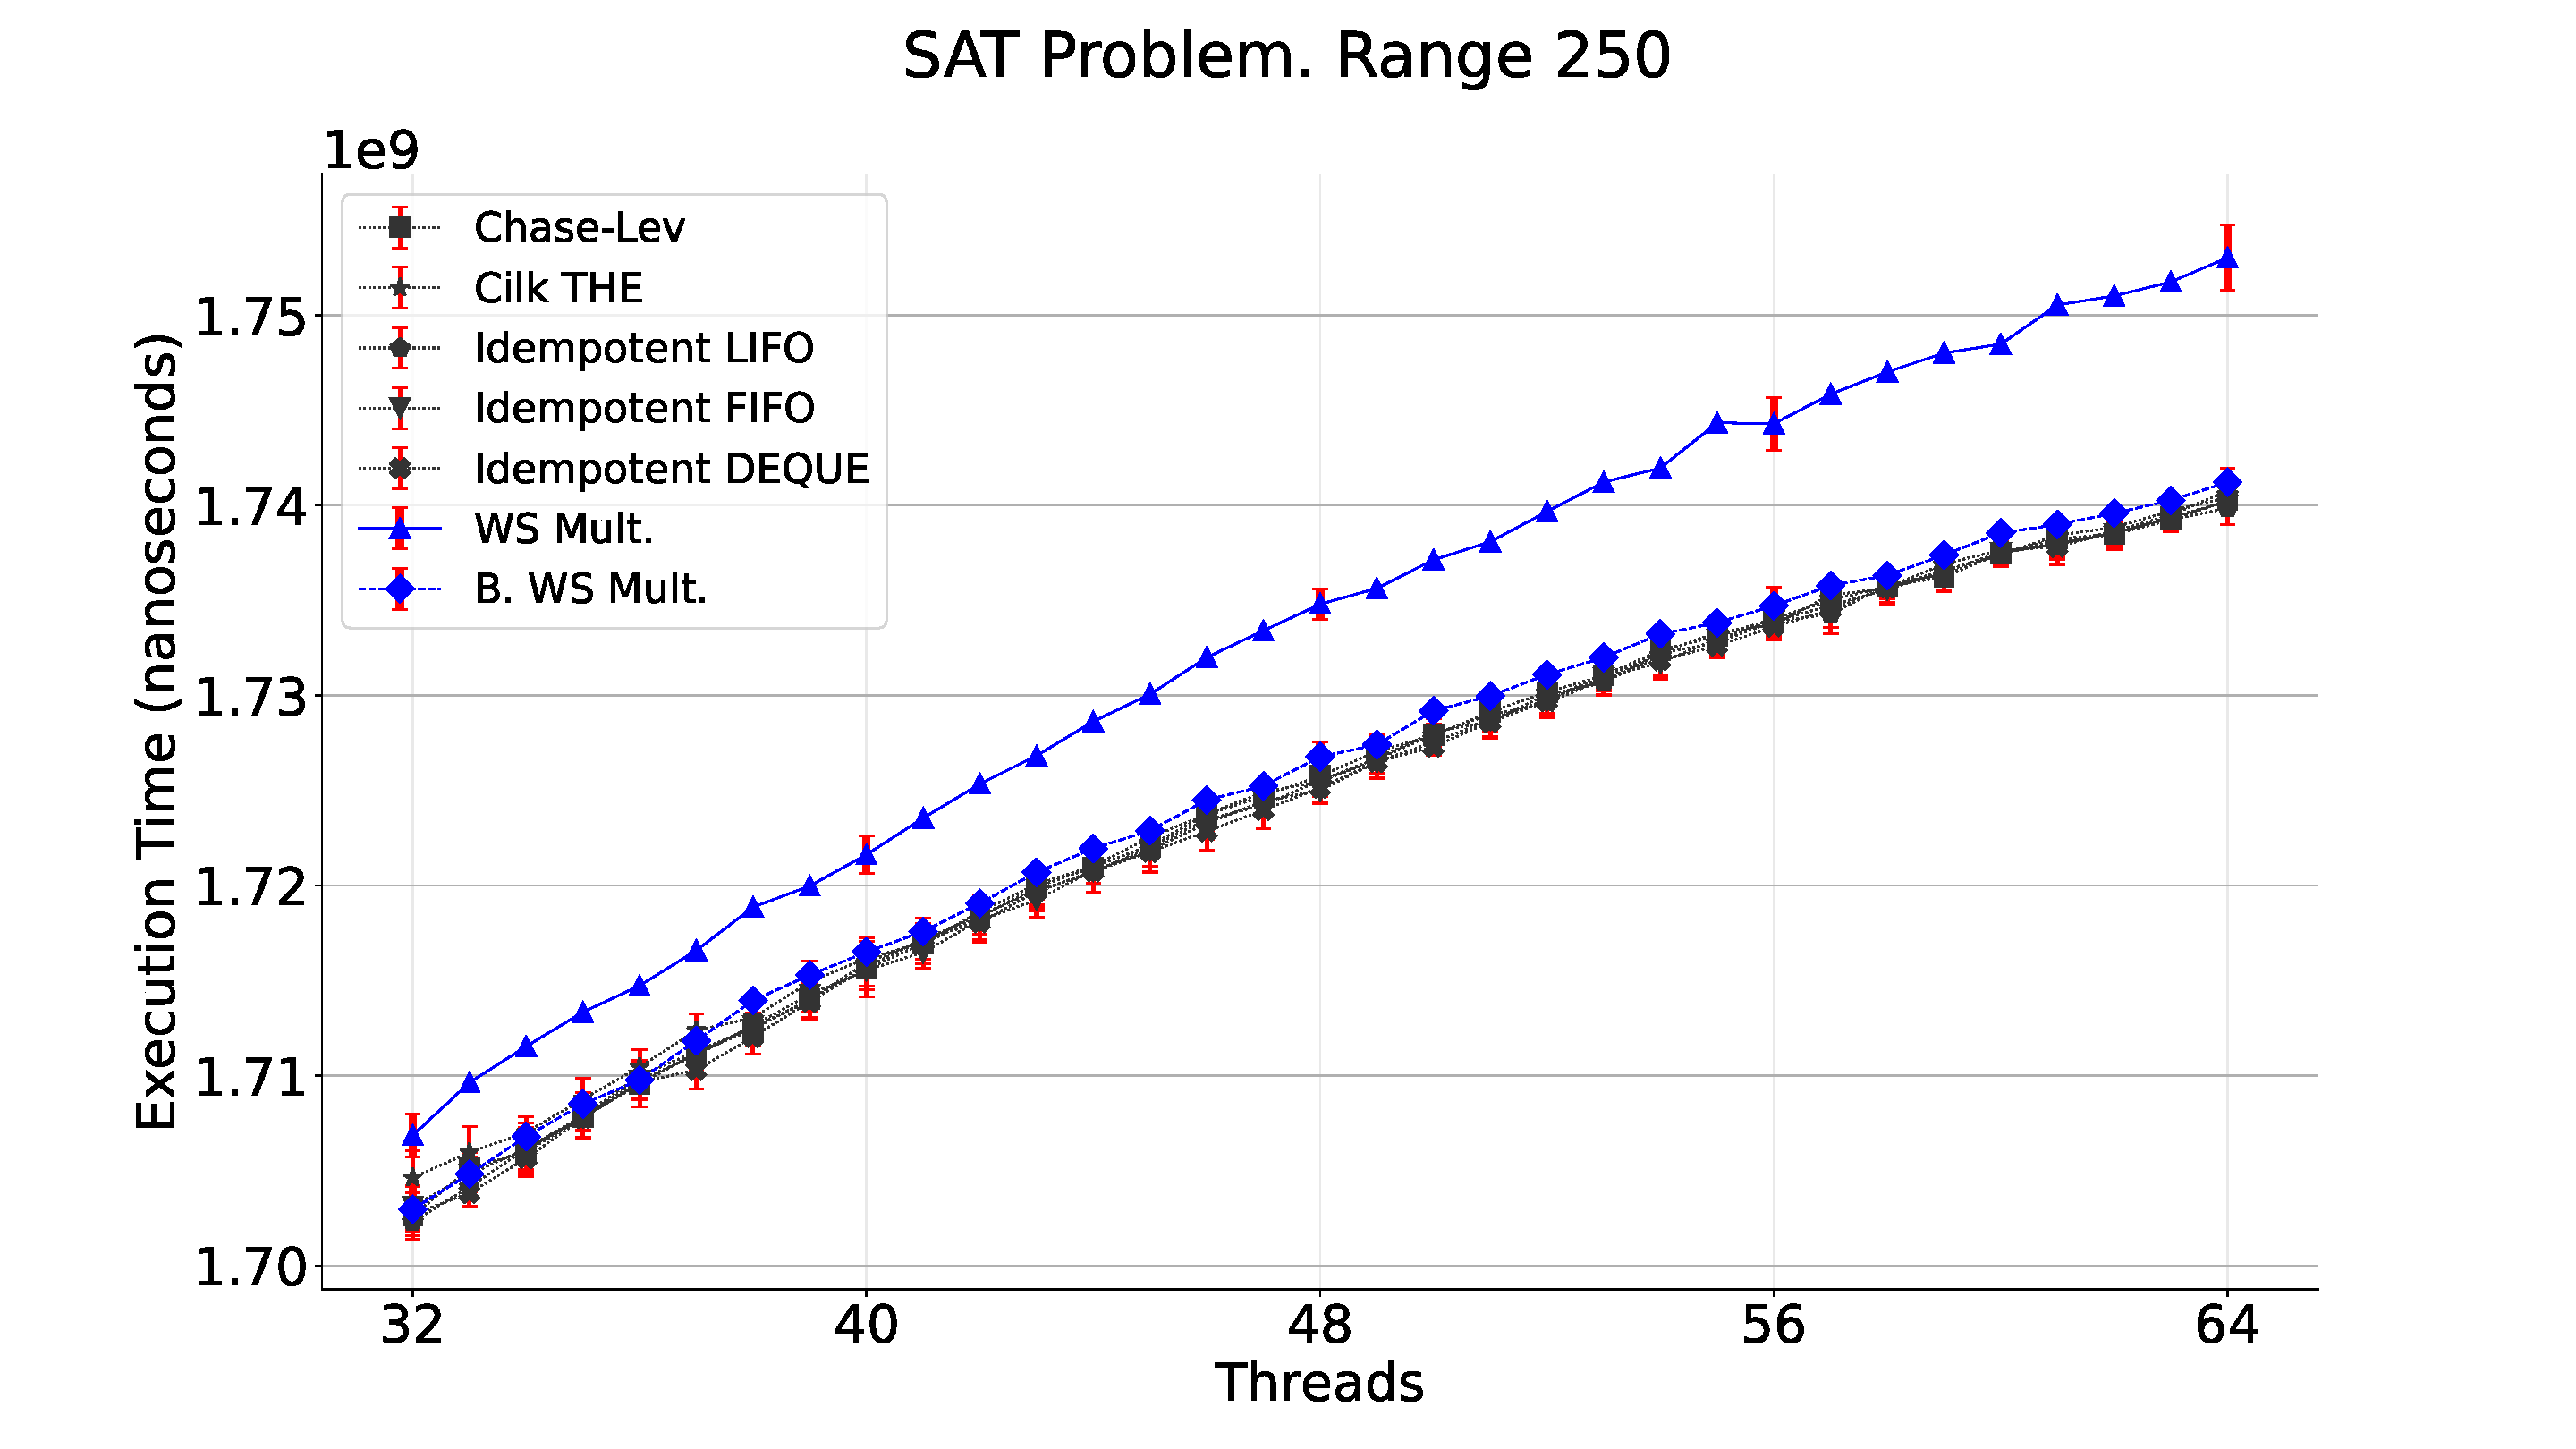
\includegraphics[width=0.48\textwidth]{contents/figures/IV_6_sat-250-2.pdf}
  }

  \subfloat[\label{fig:sat:1000:1}Range assignment size 1,000.]{
    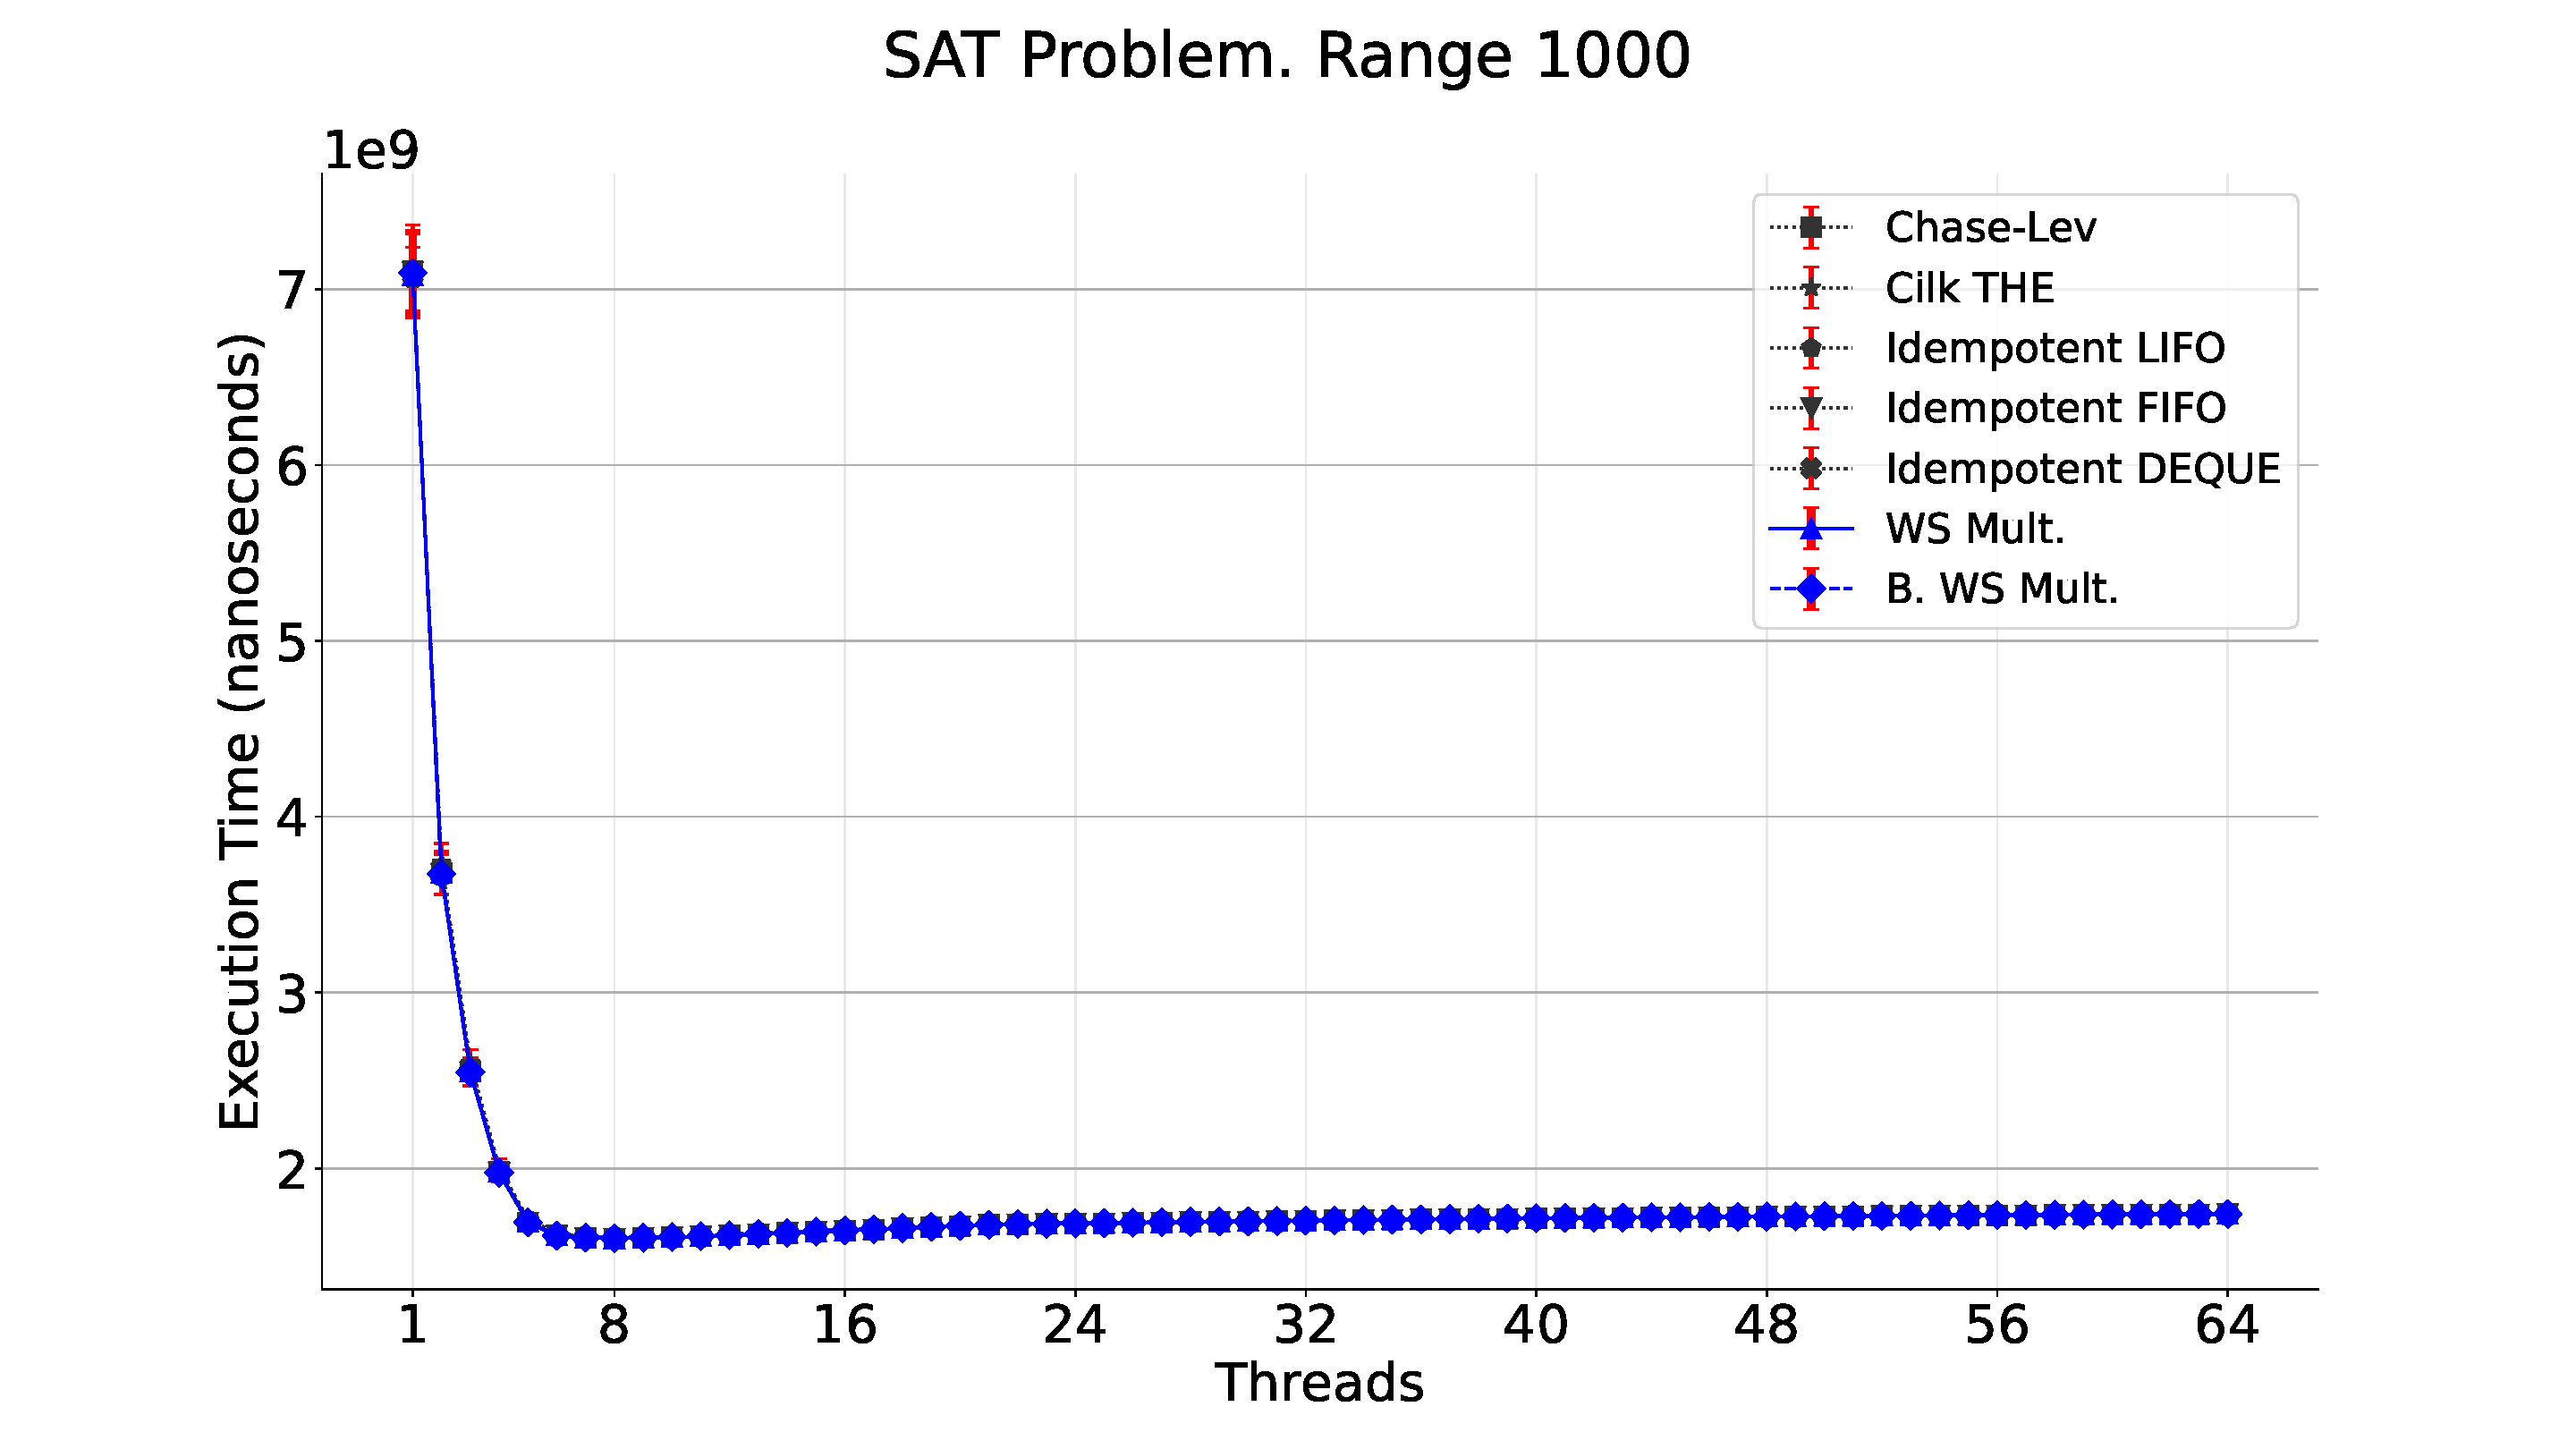
\includegraphics[width=0.48\textwidth]{contents/figures/IV_6_sat-1000-1.pdf}
  }
  \subfloat[\label{fig:sat:1000:2}Range assignment size 1,000. Zoom in to several processes 32 to 64.]{
    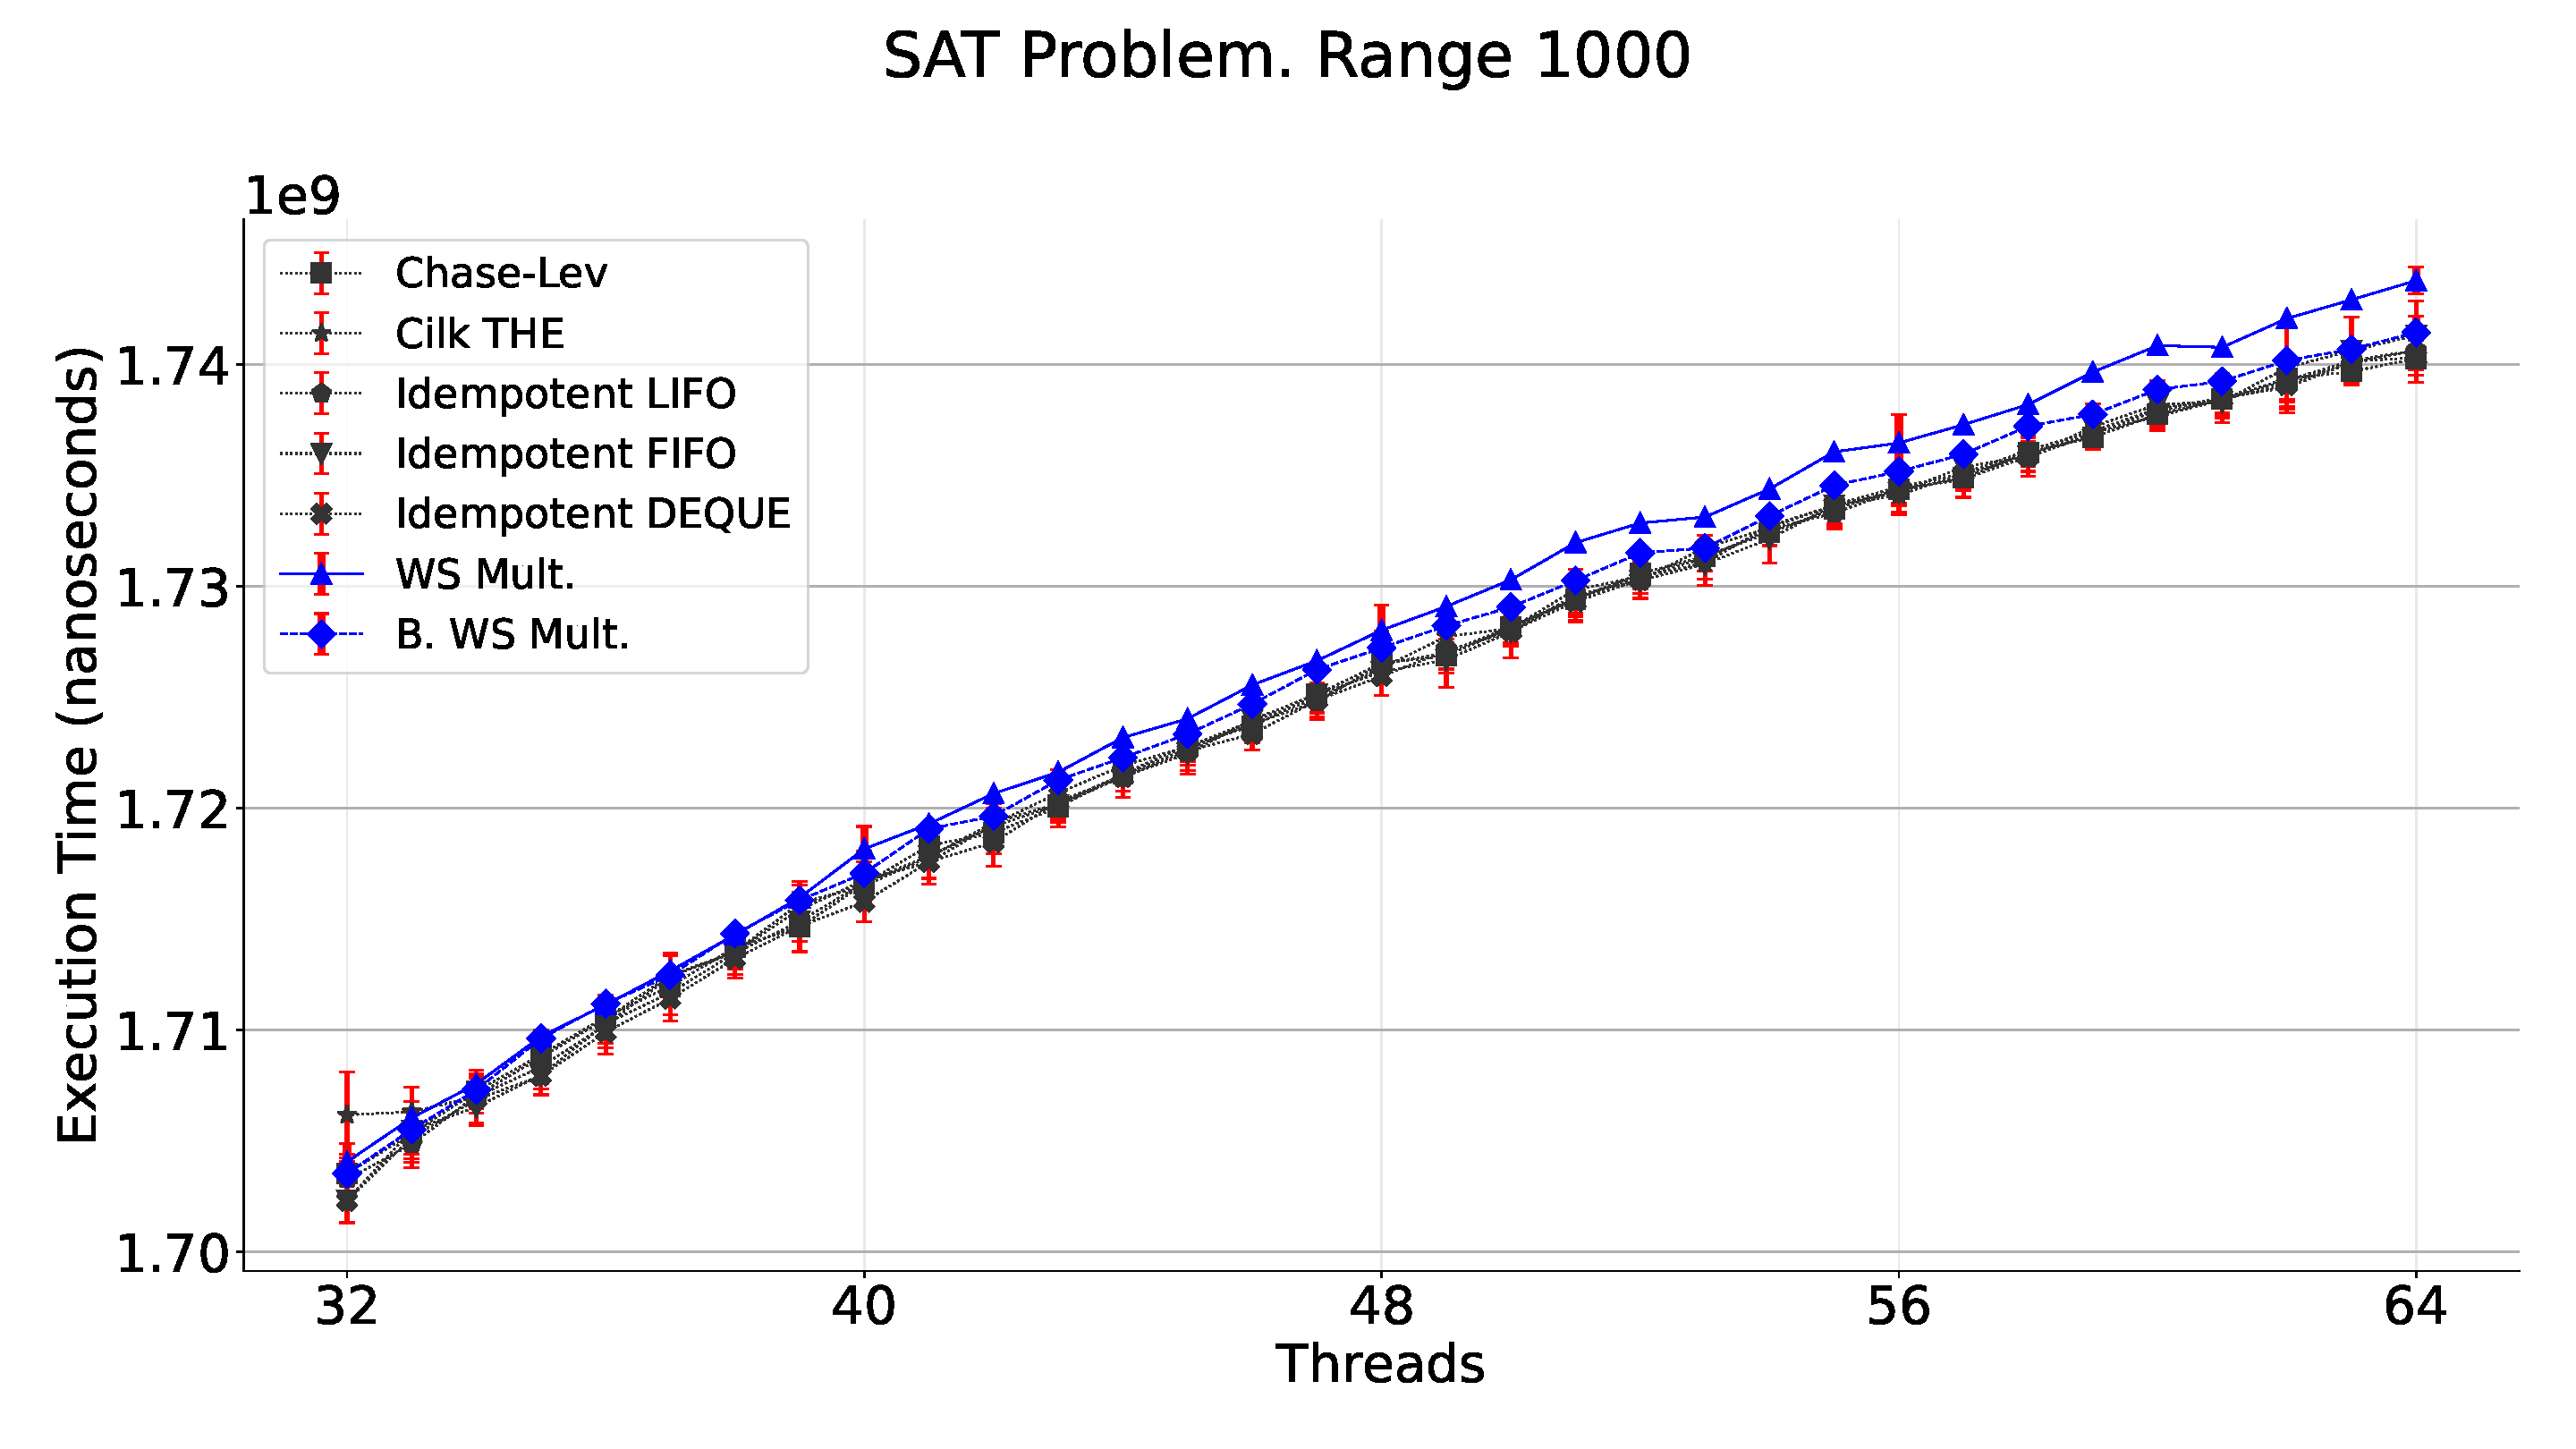
\includegraphics[width=0.48\textwidth]{contents/figures/IV_6_sat-1000-2.pdf}
  }


  \caption{\label{fig:satapplication} Mean times of the Parallel SAT benchmark for range assignment sizes 50, 250, and 1,000.}
\end{figure}

\subsection{Parallel SAT}

The outcomes for range assignment sizes 50, 250, and 1,000 are depicted in Figures~\ref{fig:sat:50:1},~\ref{fig:sat:250:1}, and~\ref{fig:sat:1000:1}, respectively. All algorithms speeded up sequential computation by 70\%, and generally, all performed similarly. However, repeated work (the difference between the number of \Puts and the number of successful \Takes/\Steals) slightly impacted the performance of \NCWSM. Contrary to previous benchmarks, whose tasks are simple, tasks in this benchmark require more computation; hence, repeated work is costly. In the experiment with range size 50, \NCWSM's repeated work was more significant than all other algorithms, and this tendency becomes more pronounced as the number of processes increases. This happens because (1) a small range size increases the possibilities of concurrent \Puts/\Takes and (2) interleavings of \Puts/\Takes of \NCWSM, where multiplicity arises, are arguably not too complex. However, repeated work was always low, less than $1\%$. Still, the small amount of repeated work had some minor impact on \NCWSM's performance.  (see Figure~\ref{fig:sat:50:2}).  For larger range sizes, 250 and 1,000, the amount of repeated work of \NCWSM decreased to almost zero (as concurrent \Puts/\Takes are less likely to happen), and hence its impact became negligible (see Figures~\ref{fig:sat:250:2} and~\ref{fig:sat:1000:2}). In contrast, idempotent algorithms had low amounts of repeated work in all cases (always close to zero), which happened because the interleaving where the relaxation appears is less likely to occur. All algorithms performed similarly when the range sizes are more significant, 250 and 1,000. It is worth stressing those insert/extract policies did not affect performance, as all tasks were generated at the beginning of the experiment; hence, every \Take/\Steal had to read from the main memory in each of these operations.

The outcomes of the rest of the experiments, for range assignment sizes 100, 500, and 2,500, are similar.  %~\ref{sec:sat-appendix} contains all results of the benchmark.

\section{Modular Basket Queues}

First, we present a summary of the experimental evaluation results from the Case Of Study presented in Chapter~\ref{chapter:5_modular-basket-queues}.

\begin{itemize}
    \item \textit{Inner experiments}:
    \begin{itemize}
        \item  \textit{LL/IC performance evaluation}: In this experiment, taking as reference the \FAI instruction performance, we measure the time of the \LL/\IC objects to perform \(1\cdot 10^6\) operations \CAS-based LL/IC object had the best performance in almost all cores, followed by the mixed version of LL/IC and finally the RW-based with 64 of padding for each entry.
        \item \textit{Modular queue variants comparison}:
    \end{itemize}
    \item \textit{Outer experiments (Queue comparison)}:
\end{itemize}

\subsection{Inner Experiments - LL/IC Performance}

The outcome of the \LL/\IC performance experiments appears in the figure

\subsection{Inner Experiments - Modular Queue Variants}
\subsection{Outer Experiments}
 